% \chapter{Learning Low-Dimensional Strain Models of Soft Robots by Looking at the Evolution of Their Shape}
\chapter{Learning Low-Dimensional Strain Models based on the Shape Evolution}
\label{chp:pcsregression}

\begin{foreword}
    % As laid out in Chapter~\ref{chp:background}, dynamical models for soft robots are derived by first settling on a parametrization of its configuration (i.e., by defining the kinematic model). Currently, it is up to the modeling engineer's intuition and trial and error to decide and tune such a model. However, besides deciding on the strain model approach (e.g., \gls{PCC}, \gls{PCS}, \gls{PAC}, \gls{GVS}, etc.), we also need to decide about other model-specific parameters. For example, for kinematics based on the \gls{PCS} approximation, we need to select how many segments the backbone is made up, the length of each segment, and the active strains per segment. Indeed, as we demonstrated already in Chapter~\ref{chp:hsamodel}, these choices (e.g., the active strains) indeed have a significant influence on the accuracy of the shape approximation and, with that, the quality of the dynamic model. Furthermore, there exists inherently a trade-off between the model complexity (i.e., the \gls{DOF} of the model) and the model performance, which is currently not sufficiently appreciated by the soft robotics modeling community.
    % For these reasons, we identify the need for an automated algorithm to analyze the before-mentioned trade-off thoroughly and, based on this analysis, choose a suitable kinematic model.
    % Finally, we desired a method that would enable us to derive a dynamic model and efficiently identify its associated parameters from data.
    % Importantly, during this learning process, we strive to preserve the interpretation and structure of these physics-based models.
    % In this chapter, we present an approach for this problem setting that consists of two steps: first, the \emph{Kinematic Fusion} algorithm automatically identifies a suitable \gls{PCS}-based kinematic parametrization based on pose samples of the backbone shape. Secondly, the \emph{Dynamic Regression \& Sparsification} algorithm allows us to identify the parameters of a physics-based dynamic model in closed form. It simultaneously reduces the model complexity by eliminating strains that can be neglected.
    % This strategy allows us to preserve the full interpretability of a physics-based \emph{white-box} model while learning the associated parameters in a data-driven fashion.
    % 
    As discussed in Chapter~\circled{\ref{chp:background}}, dynamical models for soft robots are developed by first establishing a parametrization of their configuration (i.e., defining the kinematic model). Currently, the process of selecting and fine-tuning such a model largely relies on the modeling engineer’s intuition and iterative adjustments. Beyond selecting the strain model approach (e.g., \gls{PCC}, \gls{PCS}, \gls{PAC}, \gls{GVS}, etc.), it is also necessary to determine other model-specific parameters. For instance, when using kinematics based on the \gls{PCS} approximation, decisions must be made regarding the number of backbone segments, the length of each segment, and the active strains per segment. As demonstrated in Chapter~\circled{\ref{chp:hsamodel}}, these choices—such as the selection of active strains—significantly impact the accuracy of the shape approximation and, consequently, the quality of the dynamic model. Moreover, there is an inherent trade-off between model complexity (i.e., the \gls{DOF} of the model) and model performance, a consideration that is currently underappreciated within the soft robotics modeling community.
    To address these challenges, we recognize the need for an automated algorithm that thoroughly analyzes this trade-off and selects an appropriate kinematic model based on the analysis. Additionally, we seek a method capable of deriving a dynamic model and efficiently identifying its associated parameters from data. Crucially, we aim to preserve the interpretability and structure of these physics-based models throughout the learning process.
    In this chapter, as described in Sec.~\ref{sec:pcsregression:methodology}, we propose a two-step approach to tackle this problem. First, the \emph{Kinematic Fusion} algorithm automatically determines a suitable \gls{PCS}-based kinematic parametrization using pose samples of the backbone shape. Second, the \emph{Dynamic Regression \& Sparsification} algorithm identifies the parameters of a physics-based dynamic model in closed form while simultaneously reducing model complexity by eliminating negligible strains. This approach enables us to maintain the interpretability of a physics-based \emph{white-box} model while learning its parameters in a data-driven manner. Finally, it allows us in Sec.~\ref{sub:pcsregression:validation:model_based_control} to leverage P-satI-D+Feedforward controllers, as already applied to the physics-based \gls{HSA} model in Chapter~\circled{\ref{chp:hsacontrol}}, for model-based shape regulation of the soft robot.
\end{foreword}

\pagebreak

\begin{abstract}
    Obtaining dynamic models of continuum soft robots is central to the analysis and control of soft robots, and researchers have devoted much attention to the challenge of proposing both data-driven and first-principle solutions.
    Both avenues have, however, shown their limitations; the former lacks structure and performs poorly outside training data, while the latter requires significant simplifications and extensive expert knowledge to be used in practice. This paper introduces a streamlined method for learning low-dimensional, physics-based models that are both accurate and easy to interpret. We start with an algorithm that uses image data (i.e., shape evolutions) to determine the minimal necessary segments for describing a soft robot's movement. Following this, we apply a dynamic regression and strain sparsification algorithm to identify relevant strains and define the model's dynamics. 
    We validate our approach through simulations with various planar soft manipulators, comparing its performance against other learning strategies, showing that our models are both computationally efficient and 25x more accurate on out-of-training distribution inputs.
    Finally, we demonstrate that thanks to the capability of the method of generating physically compatible models, the learned models can be straightforwardly combined with model-based control policies.
\end{abstract}

\blfootnote{This chapter is partly based on \faFileTextO~\emph{R. Valadas*, \textbf{M. Stölzle}*, J. Liu, and C. Della Santina (2025). Learning Low-Dimensional Strain Models of Soft Robots by Looking at the Evolution of Their Shape with Application to Model-Based Control. In Proceedings of the 2025 IEEE 8th International Conference on Soft Robotics (RoboSoft) (pp. 1-8). IEEE.}~\cite{valadas2025learning}.
}


%% Start the actual chapter on a new page.
\newpage

\section{Introduction}
% Continuum soft robot's inherent compliance and embodied intelligence make them promising candidates for close collaboration between humans and robots and contact-rich manipulation~\citep{rus2015design, mengaldo2022concise}.
\dropcap{M}odeling the dynamical behavior~\citep{armanini2023soft} of soft robots with computationally tractable models is important for many applications, such as efficient simulation~\citep{alkayas2025soft}, model-based control~\citep{della2023model}, state estimation~\citep{shao2023model}, and co-design~\citep{wang2024diffusebot}. 
%
% To fully exploit their potential, we need to be able to effectively control their dynamic motion.
% The complex and underactuated nature of continuum soft robots renders methods that are able to directly learn the control policy through experience~\citep{chen2024data} (e.g., \gls{RL}~\citep{thuruthel_model-based_2019, bianchi2023softoss, jitosho2023reinforcement}, Iterative Learning control~\citep{pierallini2023provably}) very interesting. However, they usually lack safety guarantees, are sample inefficient, and exhibit poor performance outside their training set distribution.
% Another avenue is to first model the dynamic behavior of the soft robot and subsequently leverage established model-based control techniques such as PD+feedforward~\citep{della2023model} or \gls{MPC}~\citep{alora2023data} to determine the control input.
% 
Developing such (low-dimensional) dynamic models is challenging and is an active area of research~\citep{alora2023data, armanini2023soft}. The use of data-driven approaches has been extensively investigated in this context~\citep{thuruthel2017learning, bruder2020data, alora2023data, chen2024data}.
These learned models exhibit poor extrapolation performance~\citep{kim2021review}, a lack of interpretability, and (physical) structure preventing us from directly leveraging closed-form control solutions such as the PD+feedforward~\citep{della2023model}. Instead, researchers had to fall back to computationally expensive planning methods such as \gls{MPC}~\citep{bruder2020data, alora2023data}.

The traditional avenue established by the robotics and continuum dynamics communities has been to derive the dynamical model directly from first principles~\citep{renda2018discrete, gazzola2018forward, grazioso2019geometrically, boyer2020dynamics, della2023model, armanini2023soft} 
which provides physical interpretability and structure at the cost of needing substantial expert knowledge, for example, in the selection of the proper kinematic approximations (e.g., \gls{PCC}~\citep{webster2010design}, \gls{PCS}~\citep{renda2018discrete}, \gls{GVS}~\citep{boyer2020dynamics}). % and the faithful integration of its geometrical, inertial, and elastic characteristics~\citep{armanini2023soft}.
%Any suboptimal choices or \emph{mistake} in this approximation \& modeling procedure can have significant consequences, such as inaccurate predictions and/or models that are too highly dimensional.
%We also point out that this prevents the democratization of soft robots~\citep{aracri2024soft} as only specialized research laboratories have access to the necessary know-how and experience. 
%
Suboptimal choices or even errors in applying this modeling procedure can lead to significant issues like inaccurate predictions and overly complex models. This hinders the democratization of soft robots, as only specialized research labs possess the required expertise~\citep{aracri2024soft}.

Recently, there has been a community push towards integrating physical structures and stability guarantees into learned models (e.g., Lagrangian Neural Networks~\citep{liu2024physics}, residual dynamical formulations~\citep{bruder2024koopman, gao2024sim}, or oscillatory networks~\citep{stolzle2024input}) which combine benefits from both worlds: they are learned directly from data which reduces the expert knowledge that is needed but at the same time exhibit a physical structure that can be exploited for model-based control and stability analysis.
This work positions itself in this new trend of research, specifically focusing on deriving kinematic and dynamic models for continuum soft robots in a data-driven way.
%, which we believe is potentially capable of overcoming the limitations of 
%
% We adopt a similar approach, focusing on 
%


%We follow a similar philosophy but focus on deriving kinematic and dynamic models in a data-driven fashion that are specialized to continuum soft robots. 
%In particular, we propose an algorithm that can identify both the structure and parameters of the expressive \gls{PCS} model~\citep{renda2018discrete}.
%The \gls{PCS} model is both established and frequently used in the soft robotic literature and divides the soft robot's structure into segments, each assumed to have constant strain. Sometimes, the soft robot's design makes it possible to neglect some of the strains (e.g., \gls{PCC} model~\citep{webster2010design}). % For example, the popular \gls{PCC} model~\citep{webster2010design} neglects all strains but bending.
%
Indeed, deriving reduced-order kinematic representations remains the core challenge in physics-based modeling. 
%
Previous works have relied heavily on the modeling engineer's intuition and experience to make decisions on the number of \gls{PCS} segments, the length of each segment, and which strains to consider~\citep{toshimitsu2021sopra}. However, these decisions are not straightforward and could easily result in models that are higher-dimensional than necessary, or that important strains are ignored based on a wrong intuition~\citep{garg2022kinematic}.
Very recently, \citet{alkayas2025soft} proposed a data-driven algorithm to identify the optimal discrete \gls{GVS}~\citep{boyer2020dynamics} strain basis of continuum soft robots via \gls{POD}. 
% However, as it is tailored towards regressing coefficients of continuous basis functions, it requires access to prior knowledge about the terminal points of actuators for accurately capturing strain discontinuities.
However, the discrete strain basis requires careful numerical integration at runtime, and identifying the dynamical parameters (e.g., stiffness, damping coefficients) of the soft robot relies upon solving a nonlinear least-squares problem that is not always well behaved~\citep{stolzle2024experimental}.

This chapter proposes to solve these challenges by introducing an end-to-end approach that can automatically learn both a \gls{PCS} kinematic parametrization and the corresponding dynamical model, including its dynamic parameters, directly from image/Cartesian pose data.
First, a kinematic fusion algorithm aims to minimize the \glspl{DOF} of the \gls{PCS} kinematic model while preserving a desired shape reconstruction accuracy for the given discrete shape measurements in Cartesian space. In contrast to previous work~\citep{alkayas2025soft}, we do not necessitate prior knowledge about strain discontinuities.
Secondly, an integrated strategy is proposed to simultaneously sparsify the strains of the \gls{PCS} model and estimate the parameters of the dynamical model with closed-form linear least-squares.
Contrary to common symbolic regression approaches such as \gls{SINDy}~\citep{kaiser2018sparse}, we crucially preserve the (physical) structure of the Euler-Lagrangian dynamics as derived according to the \gls{PCS} model.
This feature allows the derived dynamical model to be subsequently rapidly deployed within established model-based controllers~\citep{della2023model}.

% We verify the approach in simulation in diverse scenarios, including various underlying \emph{real} kinematics (e.g., \gls{PCC}, \gls{PAC}, etc.), different soft robot topologies (i.e., different number of segments), and including process and measurement noise.
We verify the approach in simulation in a diverse set of scenarios, including different robot topologies and the performance when measurement noise is present. Impressively, the method is able to accurately perform long-horizon (\SI{7}{s}) shape predictions when being trained on \SI{4}{s} of trajectory data.
%Furthermore, we present examples of Pareto fronts that describe the tradeoff between the \gls{DOF} of the kinematic model and the shape reconstruction accuracy. Analyzing this tradeoff allows the user to choose their \emph{sweetspot} between model complexity and performance.
We benchmark the proposed approach against several state-of-the-art dynamical model learning approaches (e.g., \glspl{NODE}, \gls{CON}, \glspl{LNN}). On the training set, our proposed method exhibits a \SI{70}{\percent} lower shape prediction error than the best-performing baseline method (\gls{NODE}).
However, we find that the difference is even greater in extrapolation scenarios (i.e., actuation sequences and magnitudes unseen during training): Here, our proposed method reduces the shape prediction error on the test set by \SI{96}{\percent} compared to the best performing \gls{ML} baseline (\gls{NODE}).
% We also exhibit the significantly improved extrapolation performance.
Finally, we demonstrate how the Lagrangian structure of the identified dynamical model allows us to easily design a model-based controller that is effective at regulating the shape of the soft robot.

A video attachment presents the research idea \& methodology and contains supplementary plots and animations of the results presented in the chapter.\footnote{{\small \url{https://youtu.be/dfO-PhDIiHI}}}
\section{Preliminaries}
In the following, we will provide some background on the \gls{PCS} kinematic model and the derivation of soft robot dynamics following a Lagrangian approach, which are two fundamental topics for this research paper.

\subsection{Piecewise Constant Strain (PCS) Kinematics}\label{sec:pcsregression:pcs_model}
% The continuous nature of soft robots, characterized by their ability to deform over a continuous space, implies that their motion is governed by a set of nonlinear Partial Differential Equations (PDEs)~\cite{gazzola2018forward, della2023model}. 
% As a result, an infinite number of \gls{DOF} are required to accurately characterize their dynamics.
% To make the modeling task tractable,
% , in the first step, the \emph{slender rod} assumption (e.g., Cosserat rods) allows us to describe the behavior of continuum soft robots by considering the deformations of a 1D geometric curve that represents the soft robot's backbone~\cite{gazzola2018forward, della2023model}.
% we apply the \emph{slender rod} assumption (e.g., Cosserat rods) and spatially discretize the backbone curve into $n_\mathrm{s}$ segments of constant strain, which is referred to in the literature as the \gls{DCM}~\cite{gazzola2018forward} theory, or alternatively, \gls{PCS}~\cite{renda2018discrete}.
The \gls{PCS} model~\cite{renda2018discrete} describes the kinematics of continuum soft robots by assuming that the six elemental local backbone strains (shear, axial, bending, twist) are piecewise constant across $n_\mathrm{s}$ segments but variable in time.
We remark that other popular kinematic models for soft robots, such as Piecewise Constant Curvature (PCC)~\cite{webster2010design}, are often times a special case of the \gls{PCS} model.

% To make the modeling task tractable, several assumptions are commonly used. The first one takes advantage of the typical shape of these robots, which tend to have one physical dimension longer than the other two. The analysis of slender, elongated structures can be approximated to its central axis (backbone). The second assumption takes care of the infinite-dimensional problem by approximating the continuous deformation through a space discretization along the backbone. \gls{PCS} models are built upon both of these. The backbone is discretized into a few segments, and the local strains (bending, shear, axial and torsion) are considered constant in space, but variable in time, in each of the segments. Local strains are associated with either a pure translation or rotation along one of the axis of the reference frame attached to the end of a segment. Therefore, an analogy can be drawn between joint states in rigid robots and local strains in continuum robots: just like the pose of a rigid link is dependent on the previous joint variables, the pose at a certain point of the soft robot is dependent on the local strains of all the previous segments.   %At the end of each segment is attached a reference frame $\{S_i\}$ and its configuration is defined relative to the frame of the previous one, $\{S_{i-1}\}$.

For the planar case, the configuration of the $i$th segment is referred to as
\begin{equation}
    q_i= \begin{bmatrix}
    \kappa_{\mathrm{be},i} & \sigma_{\mathrm{sh},i} & \sigma_{\mathrm{ax},i}
\end{bmatrix}^\top \in \mathbb{R}^3,
\end{equation}
where $\kappa_{\mathrm{be},i}, \sigma_{\mathrm{sh},i}, \sigma_{\mathrm{ax},i}$ are the bending, shear, and axial strains, respectively, and $i \in \{1, \dots, n_\mathrm{s} \}$. 
Therefore, the configuration of the entire soft robot is defined as $q \in \mathbb{R}^{n_\mathrm{q}}$, where $n_\mathrm{q} = 3 n_\mathrm{s}$.
We also have access to closed-form expressions for the forward and inverse kinematics of a single constant strain segment~\cite{stolzle2024experimental}.
As a consequence, forward and inverse kinematics for the entire planar \gls{PCS} soft robot can be implemented using an iterative procedure starting at the proximal end without having to resort to differential (inverse) kinematic techniques.
Namely, the forward kinematics $\pi: \mathbb{R}^{n_\mathrm{q}} \to SE(2)$ allow us to compute the pose $\chi_j = \begin{bmatrix}
    p_{\mathrm{x},j} & p_{\mathrm{y},j} & \theta_j
\end{bmatrix}^\top = \vartheta(q,s_j)$, where $s_j \in [0, L]$ is the backbone abscissa/coordinate, $L$ is the length of the entire continuum structure in an undeformed configuration, $p_{\mathrm{x},j}, p_{\mathrm{y},j} \in \mathbb{R}$ and $\theta_j$ are the positions and orientations at point $s$, respectively.
Given $N$ poses along the backbone, we can also define the inverse kinematic mapping $\varrho: 3N \times N \to n_\mathrm{q}$ that provides us with the configuration $q = \varrho(\chi, s)$ in closed-form. Here, $q_i$ will describe the configuration of the $i$th constant strain segment connecting the $i-1$th and the $i$th markers with associated poses $\chi_{i-1}$ and $\chi_i$. This means that $n_\mathrm{s} = N -1$ in order that $\rho$ can be bijective.


% \begin{figure}[htbp]
% \centerline{\includegraphics[scale=.5]{figures/pcs_diagram_2.png}}
% \caption{Illustration of a planar \gls{PCS} segment. In light gray the segment is represented only undergoing bending deformation, with amplitude $\theta_i$. In blue, the same segment also exhibits shear and axial displacements. ${S_i}$ and ${S_{i-1}}$ denote the local frames of the current and preceding segments, respectively. $\delta L_i$ and $\delta x_i$ indicate the displacements caused by shear and axial strains.}
% \label{fig:pcsregression:pcs_diagram}
% \end{figure}

% \subsubsection{Forward Kinematics}
% Subsequently, we can leverage to kinematic model to determine the homogeneous transformation $T_{i-1}^{i}(q_i) \in SE(2)$ between the proximal and the distal segment of the $i$th segment~\cite{stolzle2024experimental}
% \begin{equation}
% \begin{split}
%     T_{i-1}^{i} =& \: \begin{bmatrix}
%         \cos \left ( \theta_{i-1}^{i} \right ) & -\sin \left ( \theta_{i-1}^{i} \right ) & p_{\mathrm{x},i-1}^{i}\\
%         \sin \left ( \theta_{i-1}^{i} \right ) & \cos \left ( \theta_{i-1}^{i} \right ) & p_{\mathrm{y},i-1}^{i}\\
%         0 & 0 & 1
%     \end{bmatrix},\\
%     p_{\mathrm{x},i-1}^{i} =& \: \sigma_{\mathrm{sh},i} \frac{\sin \left ( \theta_{i-1}^{i} \right )}{\kappa_{\mathrm{be},i}} + \sigma_{\mathrm{ax},i} \, \frac{\cos \left ( \theta_{i-1}^{i} \right ) - 1}{\kappa_{\mathrm{be},i}}\\
%     p_{\mathrm{y},i-1}^{i} =& \: \sigma_{\mathrm{sh},i} \frac{1 - \cos \left ( \theta_{i-1}^{i} \right )}{\kappa_{\mathrm{be},i}} + \sigma_{\mathrm{ax},i} \, \frac{\sin \left ( \theta_{i-1}^{i} \right )}{\kappa_{\mathrm{be},i}}\\
%     \theta_{i-1}^{i} =& \: \kappa_\mathrm{be} \, L_i
% \end{split}
% \end{equation}
% where $L_i \in \mathbb{R}_{>0}$ is the segment's length and $\chi_{i-1}^{i} = \begin{bmatrix}
%     p_{\mathrm{x},i-1}^{i} & p_{\mathrm{y},i-1}^{i} & \theta_{i-1}^{i}
% \end{bmatrix}^\top \in \mathbb{R}^3$ is the pose of the distal tip in the local frame of the proximal end of the segment: $p_{x},p_{y} \in \mathbb{R}$ refer to the x- and y-position, respectively, and $\theta \in \mathbb{R}$ denotes the orientation.
% Here, we assume that the distal end of the $i-1$th segment coincides with the proximal end of the $i$th segment. In the following, we will refer to $\chi_i \in \mathbb{R}^3$ as the pose of the tip of the $i$th segment in inertial coordinates which can be computed iteratively using the robot's forward kinematics $\vartheta_i: \mathbb{R}^{3i} \to \mathbb{R}^3$ as $\chi_i = \chi_0^{i} = \vartheta_i(q_{1:i})$, where $q_{1:i}$ are the concatenated configurations of the first $i$ segments and the corresponding homogeneous transformation from the base of the robot to the tip of the $i$th segment is given as $T_{0}^i = \Vartheta_{j=1}^{i} T_{j-1}^{j}(q_j)$.

% \subsubsection{Inverse Kinematics}
% Assuming that the pose of the distal end of each segment is known, also a closed-form solution to the inverse kinematics exists~\cite{stolzle2024experimental}, in which the configuration of each segment is iteratively determined as

% \begin{equation}
% \begin{split}
%     q_i = \varrho_i(\chi_0^i, q_{1:i-1}) = \frac{\theta_{i-1}^i}{2 \, L_i} \begin{bmatrix}
%         2\\
%         p_{\mathrm{x},i-1}^{i} - \frac{p_{\mathrm{x},i-1}^{i} \sin \left (\theta_{i-1}^i \right )}{\cos \left (\theta_{i-1}^i \right ) - 1}\\
%         -p_{\mathrm{y},i-1}^{i} - \frac{p_{\mathrm{y},i-1}^{i} \sin \left (\theta_{i-1}^i \right )}{\cos \left (\theta_{i-1}^i \right ) - 1}
%     \end{bmatrix},\\
%     T_{i-1}^{i} = T(\chi_0^i) \, T(\vartheta_{i-1}(q_{1:i-1}))
% \end{split}
% \end{equation}
% starting with the most proximal segment (i.e., $i=1$). 
% We denote with the operation \textcolor{red}{TODO}
% Here, $\varrho_i: \mathbb{R}^3 \times $ describes the inverse kinematics that identifies the configuration of the $i$th segment as a function of the inertial pose of the tip of the $i$th segment $\chi_0^i$ and the configuration of the more proximal segments $q_{1:i-1} \in \mathbb{R}^{3(i-1)}$.

% This configuration vector fully specifies the shape of the robot. Given $s \in [0,L_{0,i}]$ the coordinate along the backbone, the angle of the central axis along the segment $i$ can be determined by integration of the curvature \cite{webster2010design} via 
% \begin{align}
%     \theta_i = \int_{0}^{s} \kappa_{\text{be},i} \,dv = \kappa_{\text{be},i} s \,.
% \end{align}
% The segment's position $[p_{x,i},p_{y,i}]$ can be calculated by integrating the shear and axial strains (properly rotated) 
% \begin{align}
%     \begin{bmatrix}
%         p_{x,i}\\
%         p_{y,i}
%     \end{bmatrix} =
%     \int_{0}^{s} \begin{bmatrix}
%         \cos{\theta_i} & -\sin{\theta_i} \\
%         \sin{\theta_i} & \cos{\theta_i}
%     \end{bmatrix} \begin{bmatrix}
%         \sigma_{\text{sh},i} \\
%         1 + \sigma_{\text{ax},i}
%     \end{bmatrix} \,dv .
% \end{align}

% Knowing the above relations, the forward and inverse kinematics relating the segment's pose $\chi_i=[p_{x,i},p_{y,i},\theta_i]$ and configuration $q_i$ can be written in closed form \cite{stolzle2024experimental} as
% \begin{align} 
%     \chi_i=\begin{bmatrix}
%         p_{x,i}\\
%         p_{y,i}\\
%         \theta_i
%     \end{bmatrix}=\begin{bmatrix}
%         \sigma_{\text{sh},i} \frac{\sin({\kappa_{\text{be},i} s})}{\kappa_{\text{be},i}} + (1+\sigma_{\text{ax},i}) \frac{\cos({\kappa_{\text{be},i} s}) - 1}{\kappa_{\text{be},i}} \\
%         \sigma_{\text{sh},i} \frac{1 - \cos({\kappa_{\text{be},i}s})}{\kappa_{\text{be},i}} + (1+\sigma_{\text{ax},i}) \frac{\sin({\kappa_{\text{be},i}s})}{\kappa_{\text{be},i}} \\
%         \kappa_{\text{be},i}s
%     \end{bmatrix} ,
%     \label{eq:pcsregression:pcsregression:forward_kin_pcs}
% \end{align}
% and 
% \begin{align}
%     q_i=\begin{bmatrix}
%         \theta_i / s \\
%         \theta_i \left(p_{y,i} - \frac{p_{x,i}\sin{(\theta_i)}}{\cos{(\theta_i)}-1} \right) / 2s \\
%         -1+\theta_i \left(-p_{x,i} - \frac{p_{y,i}\sin{(\theta_i)}}{\cos{(\theta_i)}-1} \right) / 2s
%     \end{bmatrix} ,
%     \label{eq:pcsregression:inverse_kin_pcs}
% \end{align}
% respectively. Notice that \eqref{eq:pcsregression:forward_kin_pcs} and \eqref{eq:pcsregression:inverse_kin_pcs} have no singularity for $\kappa_{\text{be},i} = 0$ and $\theta_i=0$. The limit in this situation where no curvature occurs in the segment is well defined and is equal to $\begin{bmatrix}
%     \sigma_{sh} s & (1+\sigma_{ax})s & 0
% \end{bmatrix}^{\top}$ and $\begin{bmatrix}
%     0 & p_{x,i}/s & -1+p_{y,i}/s
% \end{bmatrix}^{\top}$, respectively. However, some numerical instabilities might arise in practice \cite{della2023model}. 

\subsection{Lagrangian Dynamics}\label{sub:pcsregression:lagr_dynamics}
The Lagrangian of a mechanical system as a function of the configuration $q \in \mathbb{R}^{n_\mathrm{q}}$ and the corresponding time derivative $\dot{q} \in \mathbb{R}^{n_\mathrm{q}}$ can be expressed as
\begin{equation}
    \mathcal{L}(q, \dot{q}) = \mathcal{T}(q, \dot{q}) - \mathcal{U}(q) = \underbrace{\frac{1}{2}\dot{q}^\top \, M(q) \, \dot{q}}_{\mathcal{T}(q, \dot{q})} - \underbrace{\frac{1}{2} q^\top K q - \int G(q) \: \mathrm{d}q}_{\mathcal{U}(q)},
\end{equation}
where $\mathcal{T}(q, \dot{q})$, $\mathcal{U}(q)$ are the kinetic and potential energy of the system, respectively, and $M(q) \succ 0 \in \mathbb{R}^{n_\mathrm{q} \times n_\mathrm{q}}$ is referred to as the mass matrix. $G(q) \in \mathbb{R}^{n_\mathrm{q}}$ contribute the gravitational forces and $K \in \mathbb{R}^{n_\mathrm{q} \times n_\mathrm{q}}$ represents the linear elastic stiffness of the system.
Subsequently, the Euler-Lagrangian equation can be leveraged to derive the \gls{EOM} of continuum soft robots as~\cite{della2023model, liu2024physics}
\begin{equation}
    \diffp[2]{\mathcal{L}}{{\dot{q}}}\ddot{q} + \diffp{\mathcal{L}}{{q}{\dot{q}}}\dot{q} - \diffp{\mathcal{L}}{{q}} + D\dot{q} = \tau
\end{equation}
where we are also considering the generalized dissipative forces $D\dot{q}$ and the actuation torques $\tau \in \mathbb{R}^{n_\mathrm{q}}$. 
In this work, we assume, without loss of generality, that both the stiffness matrix $K = \mathrm{diag}(k_1, \dots, k_{n_\mathrm{q}})$ and the damping matrix $D = \mathrm{diag}(d_1, \dots, d_{n_\mathrm{q}}) \succeq 0$ are diagonal.

\begin{figure}[ht]
    \center
    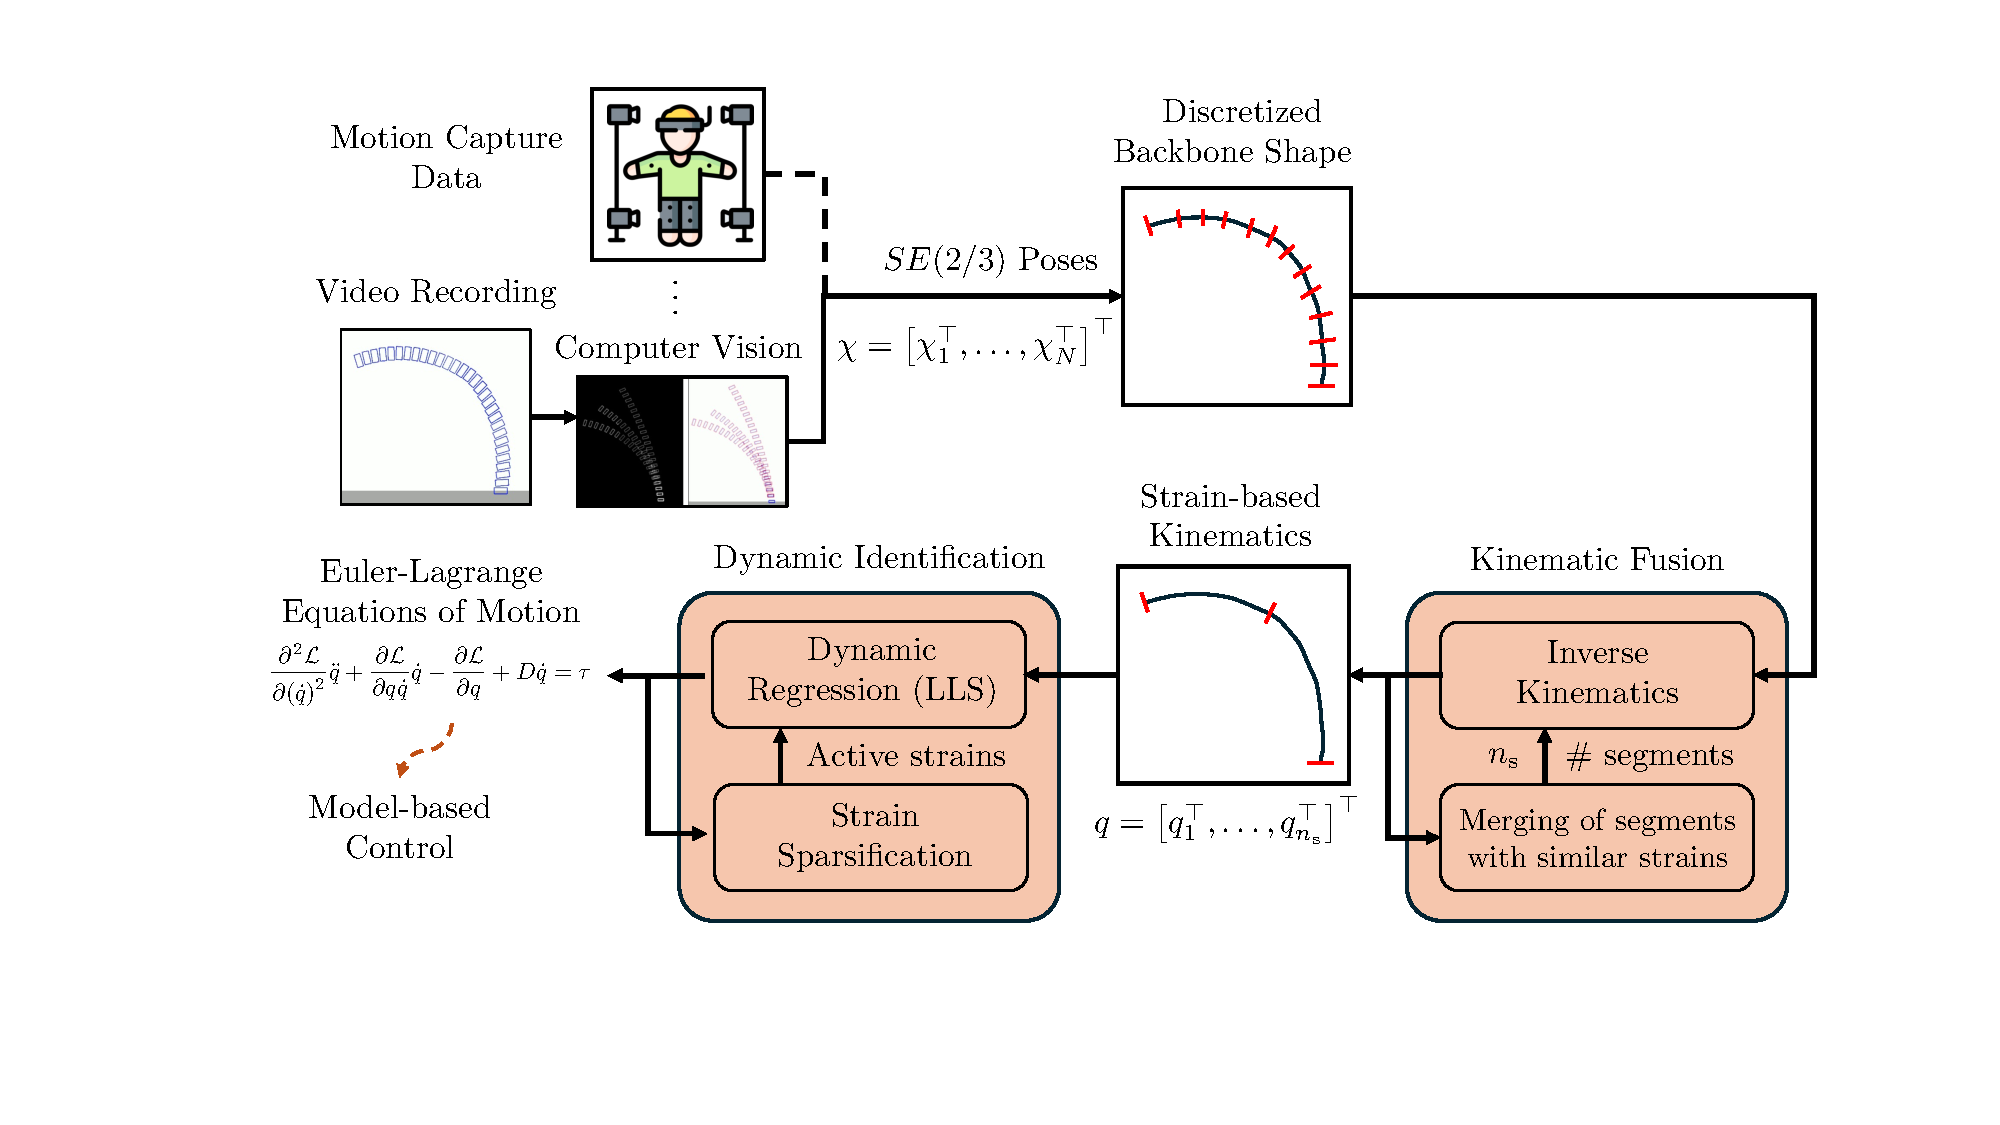
\includegraphics[width=0.9\textwidth]{pcsregression/figures/pcs_regression_overview_v2_cropped.pdf}
    \caption{
        Overview of the proposed methodology with the key contributions (\emph{Kinematic Fusion} and \emph{Dynamic Regression and Strain Sparsification}) highlighted in orange. 
        \textbf{Inputs:} We consider $N$ Cartesian pose measurements $\chi$ distributed along the soft robot backbone, for example, obtained using Computer Vision (CV) techniques from video recordings, as inputs.
        \textbf{Kinematic Fusion:} We apply an iterative procedure that involves (i) computing the robot configuration $q$ using \gls{PCS} inverse kinematics, and (ii), to avoid overly complex and high-dimensional models, we merge adjacent segments with similar strains across the dataset into one segment of constant strain.
        \textbf{Dynamic Regression:} We identify the PCS dynamic model by iteratively regressing coefficients using linear least squares and further reduce the model complexity by neglecting insignificant strains.
        \textbf{Output:} The identified dynamic model has a Lagrangian structure suitable, for example, for model-based control applications.
    }
    \label{fig:pcsregression:overall_diag}
\end{figure}

% The dynamics of a soft robot, irrespective of the kinematic model that is chosen, can be expressed in Euler-Lagrangian fashion as a function of the configuration $q \in \mathbb{R}^{n_\mathrm{q}}$ and the corresponding time derivative $\dot{q} \in \mathbb{R}^{n_\mathrm{q}}$~\cite{della2023model}
% \begin{equation}
%     M(q) \, \ddot{q} + C(q, \dot{q}) \, \dot{q} + G(q) + K q + Dq = A(q),
% \end{equation}
% where $M \in $

% The dynamics of physical systems are commonly expressed using the Lagrangian mechanics. According to this, an $n_\mathrm{q}$-DOF system can be described by a set of generalized coordinates $q \in \mathbb{R}^{n_\mathrm{q}}$, their velocities $\dot{q} \in \mathbb{R}^{n_\mathrm{q}}$, and a scalar quantity known as the Lagrangian, expressed as
% \begin{align}
%     \mathcal{L}(q, \dot{q}) = \mathcal{T}(q, \dot{q}) - \mathcal{U}(q).
% \end{align}
% The kinetic energy is given by $\mathcal{T}(q, \dot{q}) = \frac{1}{2}\dot{q}^\top \, M(q) \, \dot{q}$, with $M(q) \succ 0 \in \mathbb{R}^{n_\mathrm{q} \times n_\mathrm{q}}$ being referred to as the mass matrix. The potential energy $\mathcal{U}(q)$ includes the gravitational and elastic potential. % $V(q) = V_G(q) + V_K(q)$. % and $V_K(q) = \frac{1}{2}q^\intercal K q$ is the elastic potential, with $K \in \mathbb{R}^{n\times n}$ being the stiffness matrix. 
% Applying the principle of least action to the Lagrangian yields the Euler-Lagrangian equations which express the \gls{EOM} as
% \begin{align}\label{eq:pcsregression:euler-lagrange}
%     \diff{}{t}\left( \diffp{\mathcal{L}(q,\dot{q})}{{\dot{q}}} \right) - \diffp{\mathcal{L}(q,\dot{q})}{{q}} = F_{\text{ext}} \,,
% \end{align}
% where $F_{\text{ext}} \in \mathbb{R}^n$ represents all non-conservative forces. We here consider external forces to be restricted to velocity-dependent dissipative forces $F_{d} \in \mathbb{R}^n$ and actuation forces $F_a \in \mathbb{R}^n$, which generally are given by
% \begin{align}
%     F_{\text{ext}} = F_d+F_{a}=-D(q)\dot{q} + A(q)\tau \,,
% \end{align}
% where $D(q) \in \mathbb{R}^{n\times n}$ is the damping matrix and $A(q)\tau$ represent the actuator forces applied on the robot. $\tau \in \mathbb{R}^m$ is the control input and $A(q) \in \mathbb{R}^{n\times m}$ is the matrix that maps the point of application of the actuation to the configuration space. In this work, we will assume that $D$ is diagonal and constant and that actuators are directly collocated on the configurations, resulting in $\tau\in \mathbb{R}^n$ and $A(q)$ being the identity matrix.

% By expanding \eqref{eq:pcsregression:euler-lagrange} and after some manipulation, this set of equations can be rearranged into a more convenient matrix form,
% \begin{align}
%     M(q)\ddot{q} + C(q,\dot{q})\dot{q} + G(q) + Kq + D\dot{q} = \tau\,.
% \end{align}
% Here, $C(q,\dot{q})\dot{q} \in \mathbb{R}^n$ represents the Coriolis and centrifugal force contribution, while $G(q) \in \mathbb{R}^n$ and $Kq$ denote the gravitational and elastic actions, where $K \in \mathbb{R}^{n\times n}$ is the diagonal stiffness matrix.
% % \begin{align}
% %     G(q)=\diffp{V_G}{{q}} ,\,\, K(q)=\diffp{V_K}{{q}} .
% %\end{align}

% This dynamic formulation can be derived for a \gls{PCS} soft robot parametrization by combining its kinematic model with the inertial and impedance properties of its structure. The details for the derivations of each of these terms can be found in \cite{della2023model}.%Appendix \ref{ap:dynamics_pcs}.

% \begin{figure*}[ht]
%     \center
%     \subfigure[Kinematic Fusion Scheme]{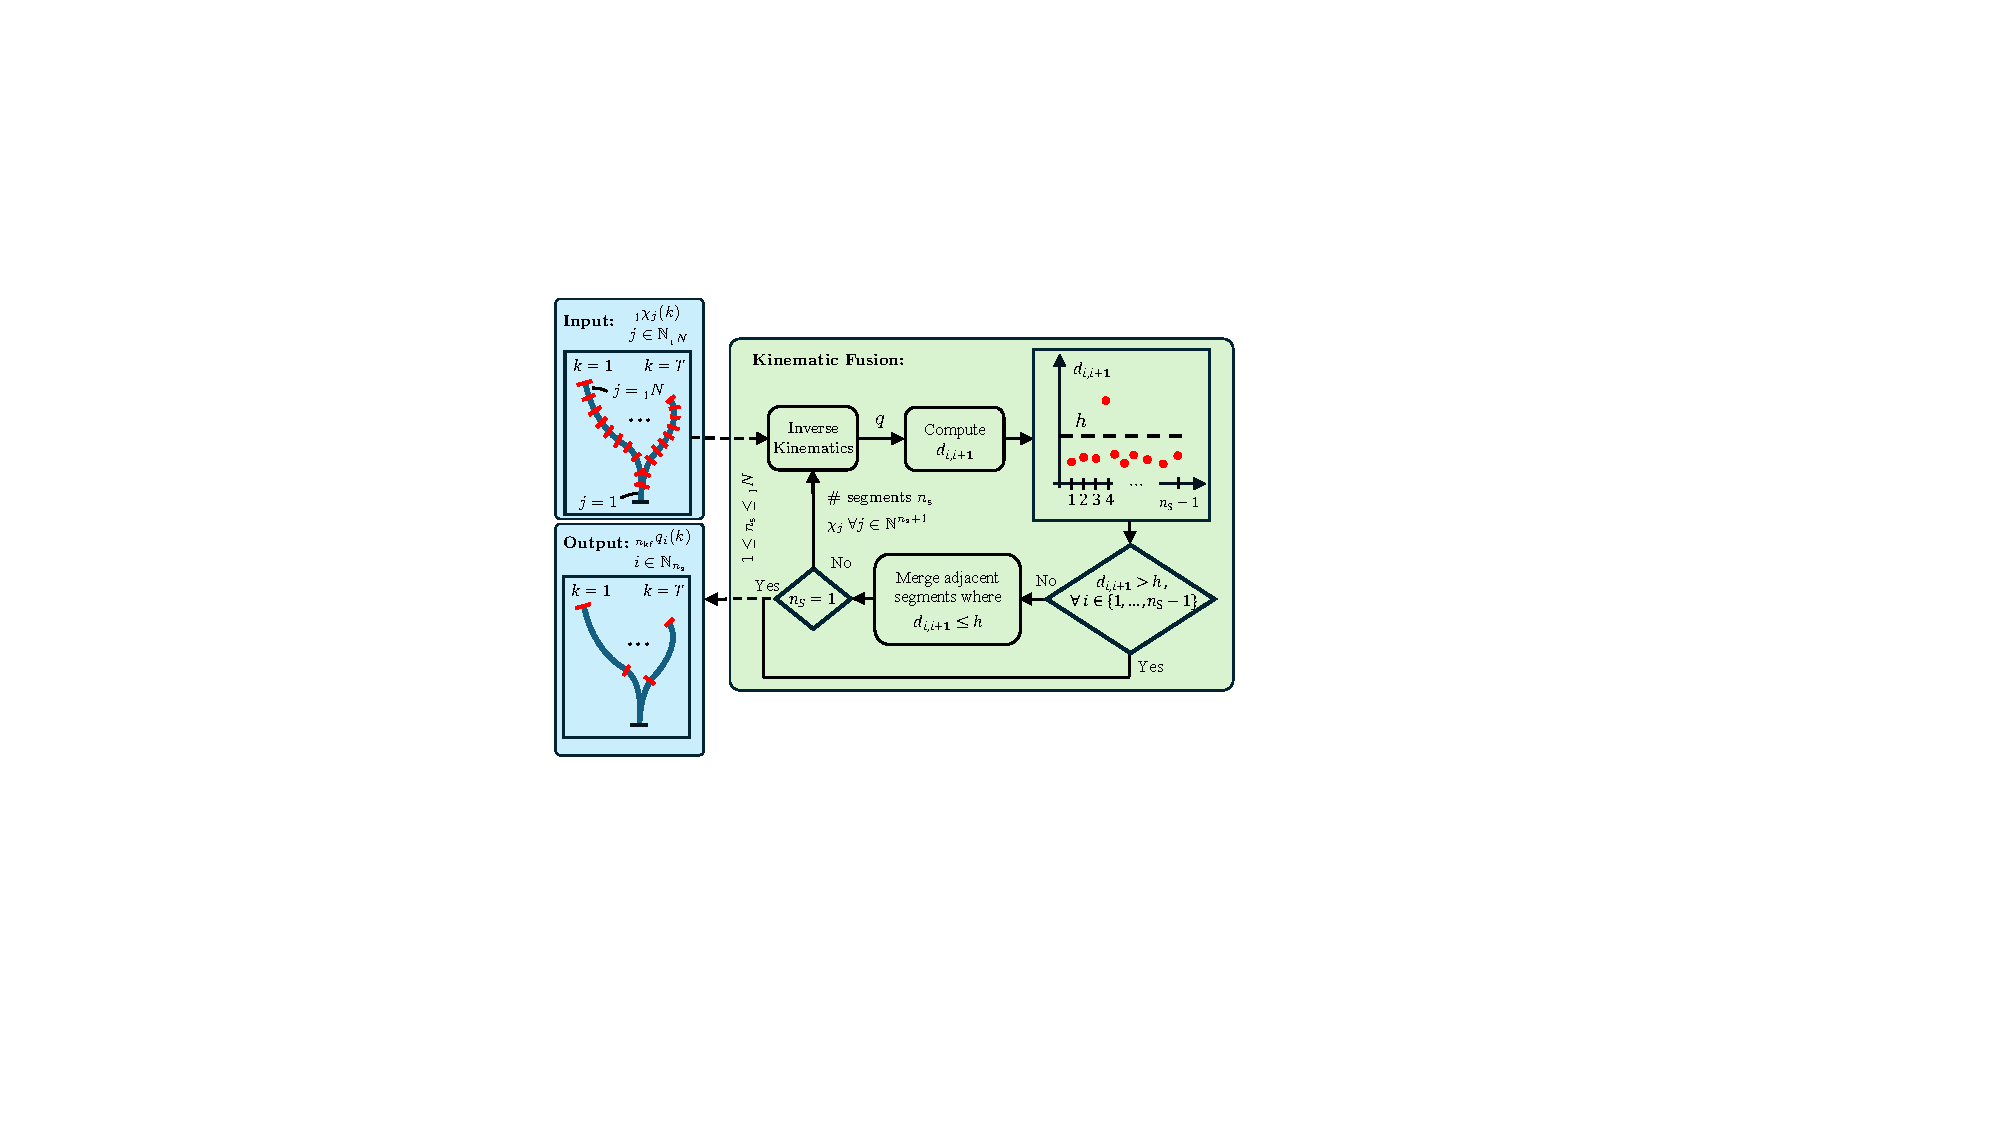
\includegraphics[width=0.34\textwidth]{pcsregression/figures/diagram_kinematic_fusion_v3_cropped.pdf}\label{fig:pcsregression:kin_regr}}
%     \hfill
%     \subfigure[Dynamic Regression \& Strain Sparsification Scheme]{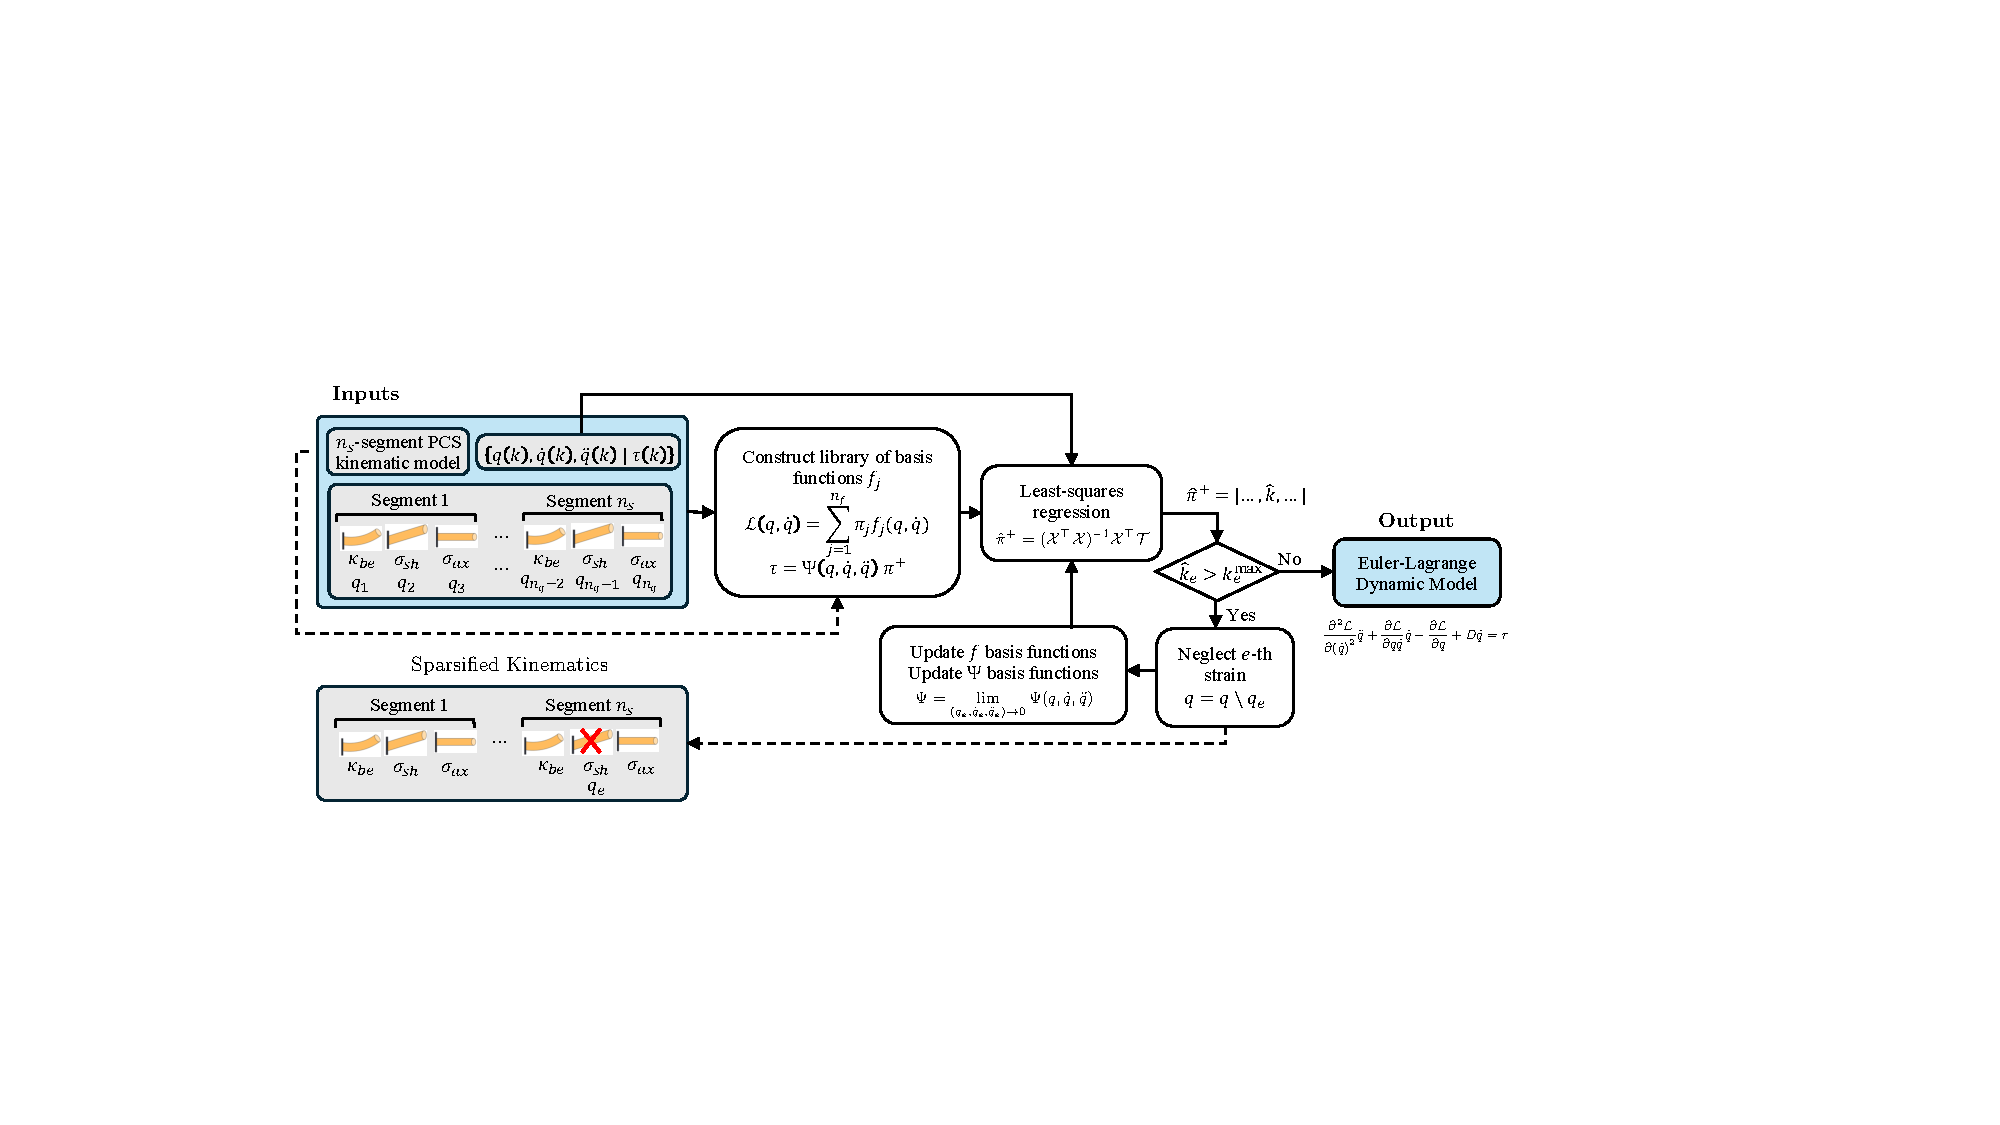
\includegraphics[width=0.65\textwidth]{pcsregression/figures/diagram_dynamic_regression_v2_cropped.pdf}\label{fig:pcsregression:dyn_regr}}
%     \caption{\textbf{Panel (a):} Schematic of the kinematic fusion algorithm. As inputs serve a sequence of $N$ discrete poses along the backbone of the soft robot. Next, we execute inverse kinematics in closed form with a $n_\mathrm{s} = N-1$ segment \gls{PCS} model to identify the (unmerged) configuration of the robot. Initially, each constant strain segment connects two neighboring backbone poses. Subsequently, we compute a strain similarity measure $\bar{d}_{i,i+1}$ between each pair of adjacent segments. If segments exhibit a similar strain (i.e., the metric falls below a threshold $h$), we merge them into one constant strain segment. This process is repeated until no more merging is possible, resulting in a kinematic model with (hopefully) fewer segments: $1 \leq n_\mathrm{s} \leq N-1$. 
%     \textbf{Panel (b):} Schematic of the dynamic model identification process that simultaneously regresses the dynamic parameters and neglects unimportant strains. Based on a $n_\mathrm{s}$-segment PCS model, a library of basis functions is constructed to parameterize the system’s Lagrangian and \gls{EOM}. A regression framework is established on a dataset of configuration-space positions $\dot{q}(k)$, velocities $\dot{q}(k)$, accelerations $\ddot{q}(k)$, and actuation torques $\tau(k)$ that estimates the dynamic parameters $\hat{\pi}^+$ with closed-form, linear least squares. Strains that exhibit a stiffness higher than a predefined threshold are neglected, prompting adjustments to the basis functions. Subsequently, this procedure is repeated until all strain stiffnesses lie below the threshold.}
% \end{figure*}
\section{Methodology}\label{sec:pcsregression:methodology}
In this work, we propose a strategy for automatically identifying low-dimensional strain models for continuum robots directly from shape trajectories, as outlined in Figure \ref{fig:pcsregression:overall_diag}.
We assume that we have access to the poses of $N$ markers along the backbone that represent a discretized shape description of the soft robot.
% These could be provided by, for example, a motion capture system or, as done in this work, extracted using computer vision techniques from images.
In this work, we primarily focus on the planar case, where we extract SE(2) poses using computer vision techniques. However, the proposed \emph{Kinematic Fusion} approach, along with the \emph{Dynamic Regression and Strain Sparsification} strategy, can be extended to 3D scenarios with SE(3) inputs. While obtaining consistent and unoccluded SE(3) poses solely from vision-based information in 3D can be challenging, it is feasible~\citep{zheng2024vision}. Additionally, SE(3) pose measurements can always be acquired through other proprioceptive~\citep{rosi2022sensing} or exteroceptive methods, such as motion capture systems.

The goal is now to identify kinematic and dynamical models that allow (a) to represent the shape with 
$n_\mathrm{s}$ \gls{PCS} segments~\citep{renda2018discrete}, where necessarily the final $n_\mathrm{s} \ll N$, and (b) to predict the future shape evolution of the soft robot.
We tackle this task by (i) identifying a low-dimensional parametrization (e.g., number of constant strain segments, the length of each segment, etc.) of the kinematics over a series of static snapshots and (ii) identifying the parameters of the Lagrangian model and simultaneously eliminating strains from the model that do not have a significant effect on the shape evolution.
We refer to component (i) as the \emph{Kinematic Fusion} algorithm as it is an iterative approach to merge parts of the backbone that exhibit a similar strain into constant strain segments.
The component (ii), named \emph{Dynamic Regression \& Strain Sparsification} algorithm, is an iterative procedure that, at each iteration, first regresses in closed-form the coefficients of the dynamic using linear least-squares and then eliminates strains from the dynamic model if the stiffness associated with a strain exceeds a given threshold. The intuition here is that strain would oscillate at very high frequencies, which are usually not relevant for practical control, and that it would take very high forces to introduce a significant deflection in the strain.
The output of our approach is low-dimensional kinematic and dynamical models that preserve the physical \& \gls{PCS} strain model structures.

% We start with images of multiple trajectories, which are processed using computer vision (CV) to estimate the poses of $N$ markers along the soft robot. An initial $N$-segment \gls{PCS} model is considered to obtain the robot's configuration through inverse kinematics. We employ a kinematic fusion procedure to reduce it to $m$ segments while preserving accuracy. Finally, dynamic model identification is performed, estimating the dynamic parameters and eliminating negligible strains, resulting in a low-dimensional model suitable for control applications.

\begin{figure}
    \centering
    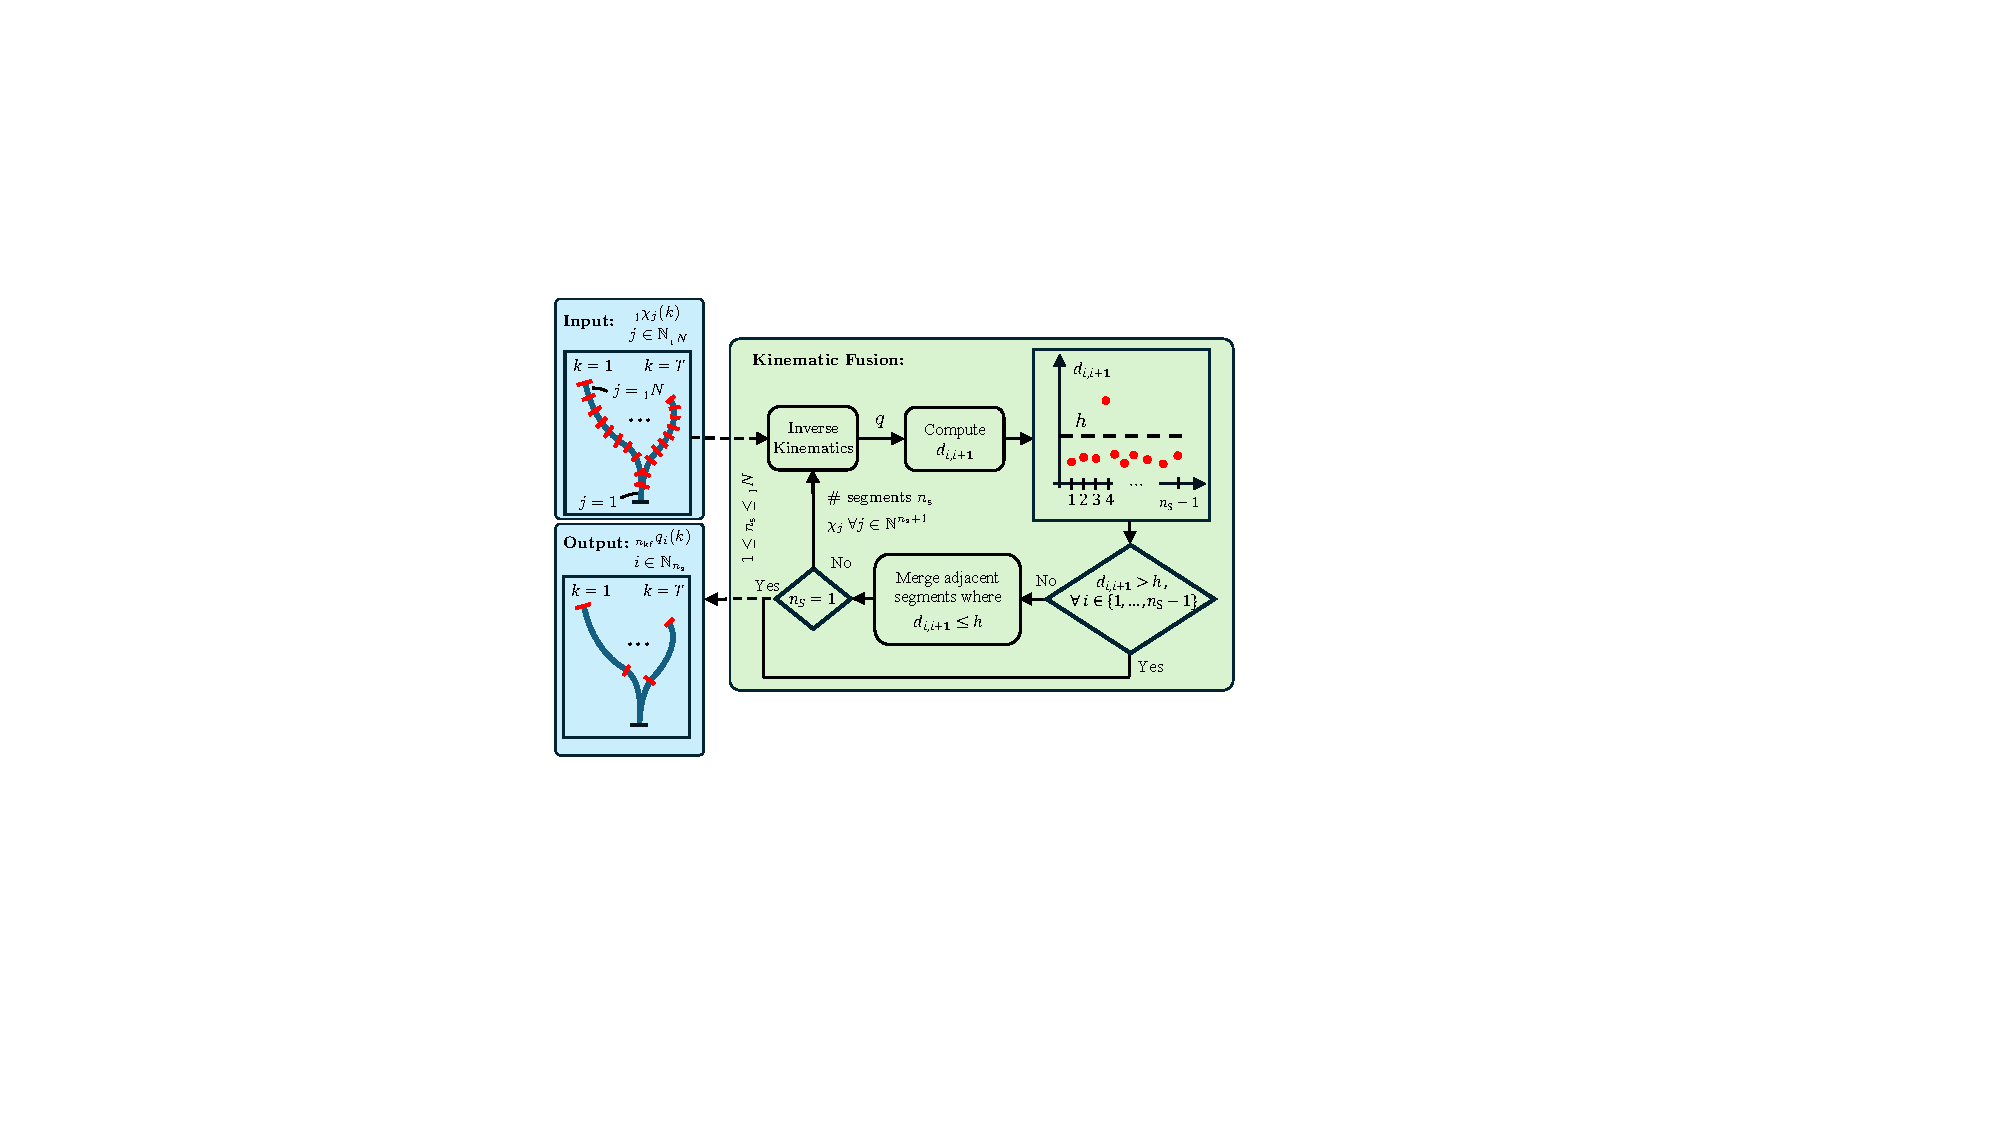
\includegraphics[width=0.7\linewidth]{pcsregression/figures/diagram_kinematic_fusion_v3_cropped.pdf}
    \caption{Schematic of the kinematic fusion algorithm. As inputs serve a sequence of $N$ discrete poses along the backbone of the soft robot. Next, we execute inverse kinematics in closed form with a $n_\mathrm{s} = N-1$ segment \gls{PCS} model to identify the (unmerged) configuration of the robot. Initially, each constant strain segment connects two neighboring backbone poses. Subsequently, we compute a strain similarity measure $\bar{d}_{i,i+1}$ between each pair of adjacent segments. If segments exhibit a similar strain (i.e., the metric falls below a threshold $h$), we merge them into one constant strain segment. This process is repeated until no more merging is possible, resulting in a kinematic model with (hopefully) fewer segments: $1 \leq n_\mathrm{s} \leq N-1$.}
    \label{fig:pcsregression:kin_regr}
\end{figure}

\subsection{Kinematic Fusion}
As previously introduced, the algorithm is provided for each training dataset sample $k \in \{1, \dots, T\}$ with $N$ pose measurements $\chi$ and associated backbone abscissas $s \in \mathbb{R}^N$ distributed along the backbone of the soft robot.
Therefore, we initialize at $l=1$: $\presub{1}{N} = N$ and $\presub{1}{\chi} = \chi$, where $l \in \mathbb{N}_{\geq 1}$ denotes the iteration index.

At the beginning of each iteration, we leverage the closed-form inverse kinematics to compute the configuration $\presub{l}{q} = \rho(\presub{l}{\chi}, \presub{l}{s}) $ of a $\presub{l}{n}_\mathrm{s} = \presub{l}{N} - 1$ segment \gls{PCS} model. We now compute between each of the total $\presub{l}{n}_\mathrm{s} - 1$ segment pairs, the following normalized strain similarity measure
\begin{equation}
    \presub{l}{\bar{d}}_{i,i+1} = \frac{1}{T} \sum_{k=1}^T \left \lVert \frac{\presub{l}{q}_{i+1}(k) - \presub{l}{q}_i(k)}{q^\mathrm{max} - q^\mathrm{min}} \right \rVert_2, \quad \forall i \in \{1, \presub{l}{n}_\mathrm{s}-1 \},
\end{equation}
where
\begin{equation}
    q^\mathrm{min} = \min_{i \in \mathbb{N}_{n}, k \in \mathbb{N}_T} q_i(k), 
    \qquad 
    q^\mathrm{max} = \max_{i \in \mathbb{N}_{n}, k \in \mathbb{N}_T} q_i(k),
\end{equation}
are the minimum and maximum configuration values across the dataset, respectively. This normalization is necessary as strains usually exhibit vastly different magnitudes. For example, the bending strains are usually more than one order of magnitude larger than the axial strains.
We keep all segment pairs with $\presub{l}{\bar{d}}_{i,i+1} > h$, where $h$ is a tunable threshold, separate. Oppositely, we merge all neighboring/adjacent segments with $\presub{l}{\bar{d}}_{i,i+1} \leq h$ into one single segment of constant strain.
If indeed $\exists \: i \in \{ \mathbb{N}_{\presub{l}{n}_\mathrm{s}} | \presub{l}{\bar{d}}_{i,i+1} < h \}$, then then kinematic model is reduced to $\presub{l+1}{n}_\mathrm{s}$ segments, where $\presub{l+1}{n}_\mathrm{s} < \presub{l}{n}_\mathrm{s}$.
As a final step of the iteration, we now subsample the Cartesian poses $\presub{l+1}{\chi}$ and the associate backbone coordinates $\presub{l+1}{s}$ such that they only contain the tip of each of the fused segments.
% As a final step of the iteration, we update the Cartesian poses using the forward kinematics to correspond to the tip of each segment: $\presub{l+1}{\chi} = \pi(\presub{l+1}{q})$

The kinematic fusion step is repeated with $l = l + 1$ for $n_\mathrm{kf}-1$ iterations until no more merging is possible, which can occur either if $\presub{n_\mathrm{kf}}{{\bar{d}}}_{i,i+1} > h \: \forall i \in \{1, \presub{n_\mathrm{kf}}{n}_\mathrm{s}-1 \}$ (i.e., the strain similarity measure is larger than $h$ for every pair of segments) or the model gets reduced to a single segment (i.e., $\presub{n_\mathrm{kf}}{n}_\mathrm{s} = 1$).
We illustrate the kinematic fusion algorithm in Fig.~\ref{fig:pcsregression:kin_regr}, and an example of the thresholding is visualized in Fig.~\ref{fig:pcsregression:results:kinematic_fusion:pcs_ns-2}.


% To develop a \gls{PCS} kinematic model for a generic soft robot, it is necessary to determine the number of segments and the length of each segment. In this work, we achieve this by means of a strain-based algorithm.

% Given that we now have access to the poses of $N$ equally distant cross-sections along the robot, we initialize an $N$-segment \gls{PCS} kinematic model, with nodes positioned at the center of the $N$ cross-sections. Essentially, each of the $N$ tracked cross-sections will consist of a segment's end section. We apply the closed-form inverse kinematics from \eqref{eq:pcsregression:inverse_kin_pcs} to map the Cartesian poses $\chi_i$ into configuration variables $q_i$. To avoid the numerical instabilities near the straight configuration ($\theta=0$), a small $\varepsilon$ is added to the bending angle. It is important to note that $[p_x,p_y,\theta]$ in \eqref{eq:pcsregression:inverse_kin_pcs} must be written with respect to the previous frame ${S_{i-1}}$. However, the computer vision step outputs all the poses $\chi_i$ with respect to the fixed frame attached to the base of the soft robot. Therefore, a mapping must be applied to go from $\prescript{0}{}{\chi}_i$ into $\prescript{i-1}{}{\chi}_i$. This is achieved using the composition operation
% \begin{align}
%     \prescript{i-1}{}{H}_i = \prescript{i-1}{}{H}_0 \prescript{0}{}{H}_i = \left(\prescript{0}{}{H}_{i-1}\right)^{-1} \prescript{0}{}{H}_i \,,
% \end{align}
% where $\prescript{0}{}{H}_i$ is the homogeneous transformation matrix that represents pose $\prescript{0}{}{\chi}_i$. For the planar case, this is given by
% \begin{align}
%     \prescript{0}{}{H}_i = \begin{bmatrix}
%         \cos{\theta_i} & -\sin{\theta_i} & p_x^i \\ \sin{\theta_i} & \cos{\theta_i} & p_y^i \\ 0 & 0 & 1
%     \end{bmatrix}\,.
% \end{align}
% Once $\prescript{i-1}{}{H}_i$ has been computed, $\prescript{i-1}{}{\chi}_i$ can be extracted from the matrix entries.

% After computing the sequence of configurations for the $N$ initial segments, we employ a recursive algorithm to determine the final number of segments $m$, where $m<N$. The idea is that adjacent segments that have similar strain trajectories (i.e., deform similarly) can be merged together and considered a single segment. Note that each local strain has distinct units (bending strain has units $\mathrm{m^{-1}}$, while shear and axial strains are unitless). In order to compute a metric that measures strain similarity over the entire strain-space, we apply a normalization by scaling each strain relative to their maximum values. In this work, the bending strain is not greater than $60 \,\mathrm{m^{-1}}$, while shear and axial strains achieve maximum values of $30\,\mathrm{\%}$.

% The metric to measure strain similarity is the average strain-space (euclidean) distance between pairs of consecutive segments,
% \begin{align}
%     \bar{d}_{i,i+1} = \frac{1}{T} \sum_{k=1}^T \left\| \bar{q}_i (k) - \bar{q}_{i+1} (k) \right\|\,,
% \end{align} 
% where $\bar{q}_i$ represent the $i$-th segment's scaled strains. 
% %Note that this metric is dependent on the strain magnitudes, which differ across the strain-space since local strains have distinct units (bending strain has units $\mathrm{m^{-1}}$, while shear and axial strains are unitless). Therefore, to ensure a more even contribution to the similarity metric from each strain, these are first scaled relative to their maximum values. In this work, the bending strain is not greater than $60 \,\mathrm{m^{-1}}$, while shear and axial strains achieve maximum values of $30\,\mathrm{\%}$.

% We compute this average strain distance for each pair of adjacent segments. For a kinematic model with $n_S$ segments, this yields $n_S-1$ pairs. If the distance $\bar{d}_{i,i+1}$ for the $i$-th pair is below or equal to a pre-defined threshold $h$, segments $i$ and $i+1$ will be grouped into a single segment. Otherwise, the segments remain separate. This results in a new \gls{PCS} kinematic model with fewer segments. Figure \ref{fig:pcsregression:kin_regr} illustrates this procedure. The configuration of each new merged segment is determined by performing a one-segment inverse kinematics on the distal ends of the merged segment.
% % averaging the (nonscaled) strains of its $c$ constituent segments, weighted by their lengths,
% % \begin{align}
% %     q_{\text{merged}} = \frac{\sum_{j=1}^c q_j L_{0,j}}{\sum_{j=1}^c L_{0,j}} \,.
% %\end{align}


% This sequence is repeated until no more merging is possible, which can occur either if $\bar{d}_{i,i+1}$ is larger than $h$ for every pair of segments or the model gets reduced to a single segment. Algorithm \ref{alg:kin_regression} illustrates an overview of all the steps.

% \begin{algorithm}
% \caption{Kinematic Regression}
% \label{alg:kin_regression}
% \begin{algorithmic}[1]
% % \REQUIRE Poses $\prescript{0}{}{\chi}_i (k)$ \COMMENT{$i=1,...,N$}
% \REQUIRE Configurations $q_i (k)$  \COMMENT{$i=1,...,N$}
% \ENSURE Configurations $q_i (k)$ \COMMENT{$i=1,...,m\,\,(m<N)$}

% % \FOR{each frame $k=1$ \TO $T$}
% % \FOR{each cross-section $i=1$ \TO $N$}
% % \STATE $\prescript{0}{}{T}_i \gets \prescript{0}{}{\chi}_i$
% % \STATE $\prescript{i-1}{}{T}_i = ( \prescript{0}{}{T}_{i-1} )^{-1} \prescript{0}{}{T}_i$
% % \STATE $\prescript{i-1}{}{\chi}_i \gets \prescript{i-1}{}{T}_i$
% % \STATE $q_i \gets \text{IK}(\prescript{{i-1}}{}{\chi}_i) $
% % \ENDFOR
% % \ENDFOR
% % \STATE
% \REPEAT
%     \STATE $\bar{q}_i \gets q_i / q_{\text{max}}$ \COMMENT{Scale $q_i$}
%     \STATE \textit{merge\_candidates} $\gets [\,]$
%     \STATE \textit{current\_merge} $\gets [1]$
%     \FOR{$i=1$ \TO $n_S-1$}
%         \STATE $\bar{d}_{i,i+1} \gets \frac{1}{T} \sum_{k=1}^T \left\| \bar{q}_i (k) - \bar{q}_{i+1} (k) \right\|$
%         \IF{$\bar{d}_{i,i+1} \leq h$}
%             \STATE Append $i+1$ to \textit{current\_merge}
%         \ELSE 
%         \STATE Append \textit{current\_merge} to \textit{merge\_candidates}
%         \STATE Reinitialize \textit{current\_merge} $\gets [i+1]$
%         \ENDIF
%     \ENDFOR
%     % \FOR{each segment pair $(i, i+1)$}
%     %     \STATE Compute $\bar{d}_{i,i+1}$
%     %     \IF{$\bar{d}_{i,i+1} < p$}
%     %         \STATE Add $(i,i+1)$ to \textit{merge\_candidates}
%     %     \ELSE 
%     %     \STATE Keep $(i,i+1)$ as separate segments 
%     %     \ENDIF
%     % \ENDFOR
%     \STATE
%     \FOR{each group in \textit{merge\_candidates}}
%     % \STATE \COMMENT{$m$ constituent segments with lengths $L_{0,j}$}
%     %\STATE \COMMENT{Compute $q_{\text{merged}}$ by averaging the configurations of the constituent segments $1,2,...,m$, weighted by their lengths $L_{0,j}$} 
%     % \STATE $q_{\text{merged}} = \sum_{j=1}^{c} (q_{j} L_{0,j} /  L_{0,j})$
%     \STATE $q_{\text{merged}} = \text{IK}(\prescript{{\text{init}}}{}{\chi}_{\text{end}})$
%     \STATE \COMMENT{$\prescript{{\text{init}}}{}{\chi}_{\text{end}}$ is the pose of the end section of the merged segment relative to the initial section}
%     \ENDFOR
% \UNTIL{$n_S=1$ \OR $\bar{d}_{i,i+1}>h\,, \forall\, i \in [1,n_S-1]$}
% \end{algorithmic}
% \end{algorithm}

\begin{figure}
    \centering
    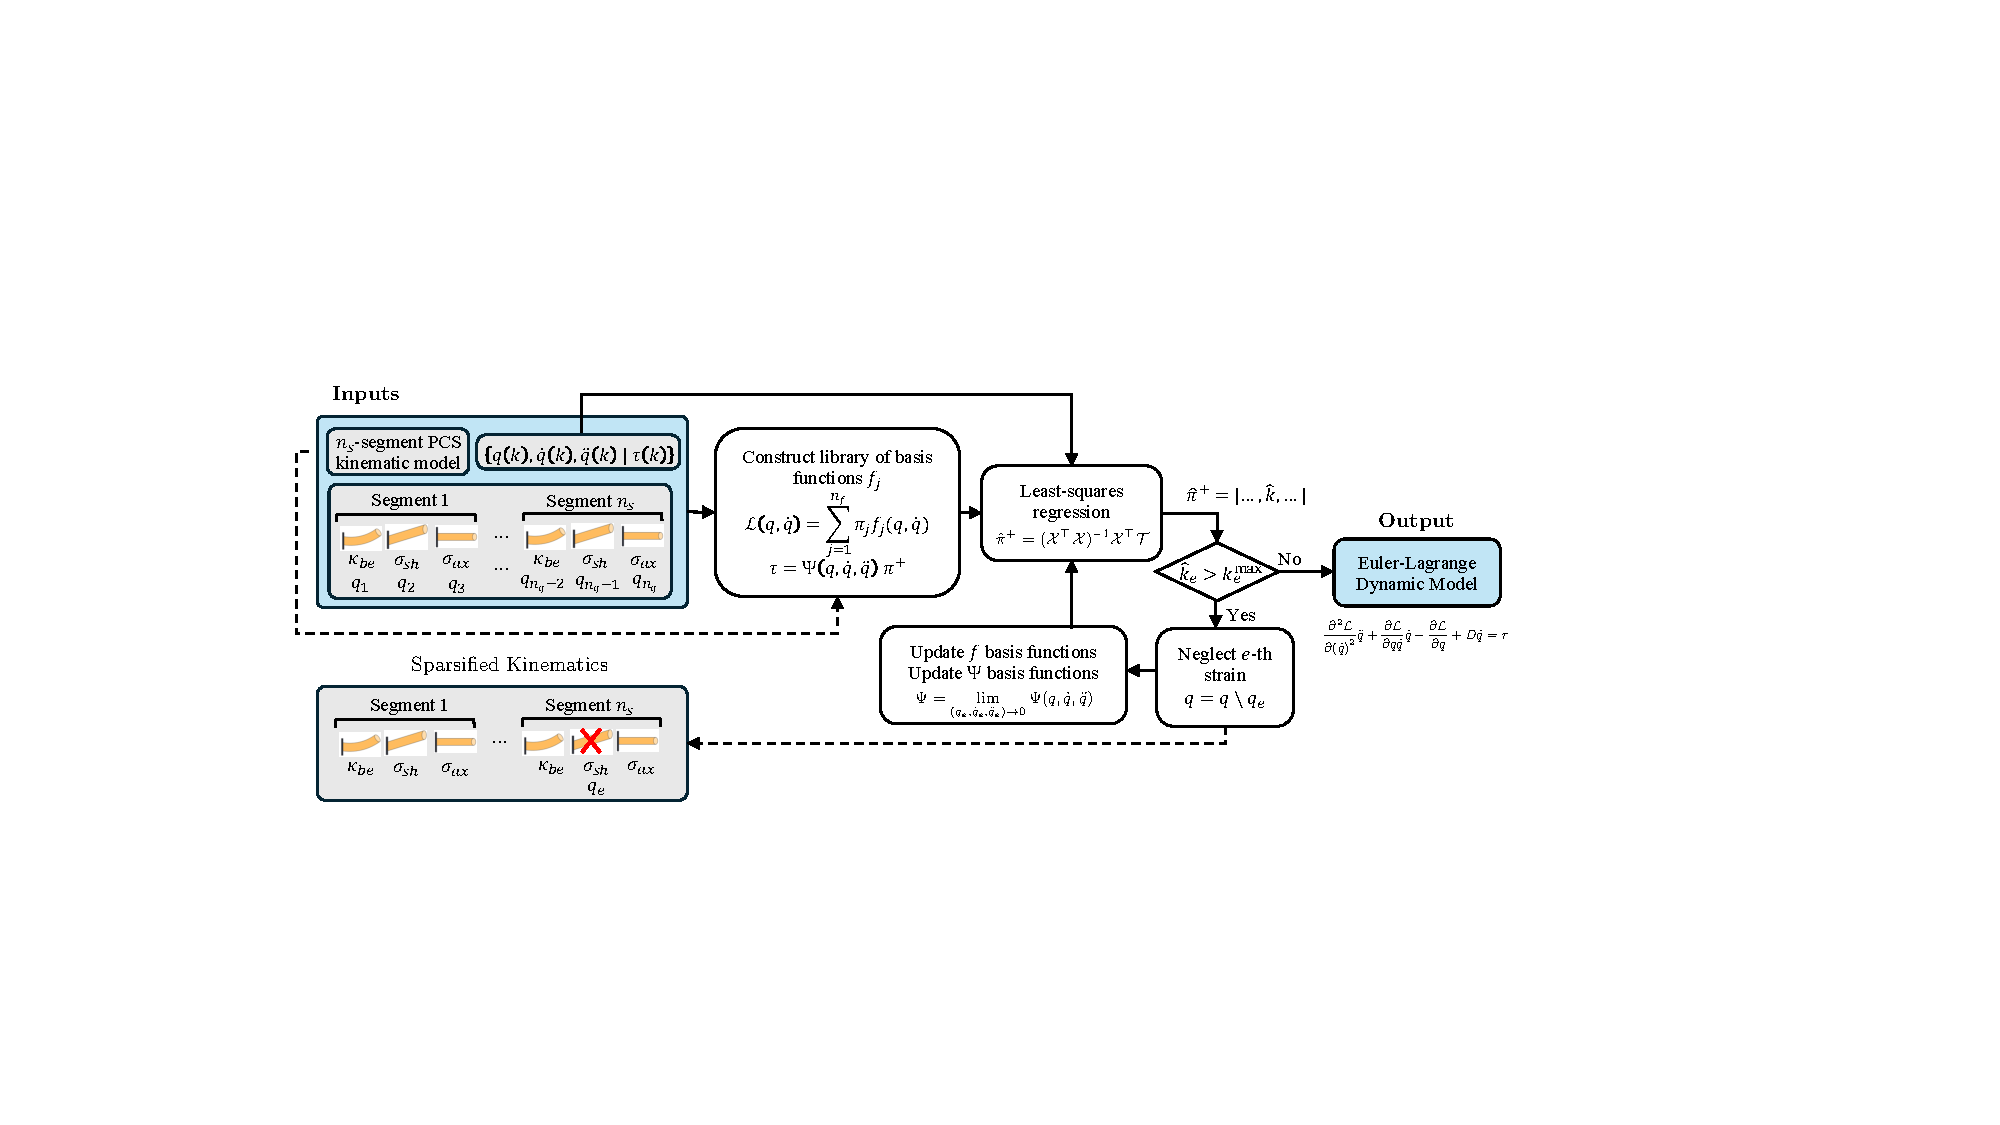
\includegraphics[width=1.0\linewidth]{pcsregression/figures/diagram_dynamic_regression_v2_cropped.pdf}
    \caption{Schematic of the dynamic model identification process that simultaneously regresses the dynamic parameters and neglects unimportant strains. Based on a $n_\mathrm{s}$-segment PCS model, a library of basis functions is constructed to parameterize the system’s Lagrangian and \gls{EOM}. A regression framework is established on a dataset of configuration-space positions $\dot{q}(k)$, velocities $\dot{q}(k)$, accelerations $\ddot{q}(k)$, and actuation torques $\tau(k)$ that estimates the dynamic parameters $\hat{\pi}^+$ with closed-form, linear least squares. Strains that exhibit a stiffness higher than a predefined threshold are neglected, prompting adjustments to the basis functions. Subsequently, this procedure is repeated until all strain stiffnesses lie below the threshold.}
    \label{fig:pcsregression:dyn_regr}
\end{figure}

\subsection{Dynamic Regression \& Strain Sparsification}
After obtaining a kinematic model with the \emph{Kinematic Fusion} algorithm, we can employ the identified parametrization as a foundation for deriving a dynamic model. % To do so, we implement a data-driven dynamic identification method that allows the extraction of a minimalistic-dimensional description of a soft manipulator.
First, we symbolically derive the basis functions of the \gls{PCS} dynamical model.
Subsequently, we implement an iterative procedure to (i) regress dynamic coefficients with linear least squares and (ii) identify strains that can be neglected and remove them from the dynamical model.

\subsubsection{Parametrization of the PCS Dynamic Model with Basis Functions}
In order to easily regress the dynamic parameters with linear least squares, we first derive the \gls{PCS} dynamics for a $n_\mathrm{s}$ segment soft robot from first principle~\citep{armanini2023soft, della2023model}, with all rotational and linear strains taken into account, and subsequently parametrize both the Lagrangian and Euler-Lagrangian equations as a linear combination of monomial basis function.
% In this work, we will perform a system identification to find the Lagrangian of the soft robot. Let us consider a soft manipulator with configuration variables $q \in \mathbb{R}^{n_q}$. We leverage the knowledge of the previously found kinematic model to parametrize the Lagrangian as a linear combination of monomial basis functions,
\begin{equation}\label{eq:pcsregression:lagrangian_basis_functions}
    \mathcal{L}(q, \dot{q}) = \sum_{j=1}^{n_\mathrm{f}} \pi_j f_j(q, \dot{q}), 
    \quad
    \tau = \sum_{j=1}^{n_\psi} \pi_j^{+}\Psi_j(q,\dot{q},\ddot{q}) \in \mathbb{R}^{n_q},
\end{equation}
where $f_j: \mathbb{R}^{n_\mathrm{q}} \times \mathbb{R}^{n_\mathrm{q}} \to \mathbb{R}$ denotes each of the basis functions, and $\pi \in \mathbb{R}^{n_\mathrm{f}}$ the corresponding coefficients.
Analog, we derive symbolically the \gls{EOM} using an Euler-Lagrangian approach (see Section~\ref{sub:pcsregression:lagr_dynamics}) and now state the corresponding basis functions as $\psi(q, \dot{q}, \ddot{q}) \in \mathbb{R}^{n_\Psi \times n_\mathrm{q}}$ with $\psi_j: \mathbb{R}^{n_\mathrm{q}} \times \mathbb{R}^{n_\mathrm{q}} \times \mathbb{R}^{n_\mathrm{q}} \to \mathbb{R}^{n_\mathrm{q}}$ such that
\begin{equation}
    \tau = \sum_{j=1}^{n_{f}} \left[ \pi_j \left( \diffp[2]{f_j}{{\dot{q}}}\ddot{q} + \diffp{f_j}{{q}{\dot{q}}}\dot{q} - \diffp{f_j}{{q}} \right) \right] + D\dot{q},
\end{equation}
where
$\pi^+ = \begin{bmatrix}
    \pi^\top & d^\top 
\end{bmatrix}^\top \in \mathbb{R}^{n_{\psi}}$ contains the associated coefficients and consists of $\pi$ and the damping coefficients $d = \mathrm{diag}(D) \in \mathbb{R}^{n_\mathrm{q}}$.

% The value $m$ denotes the number of segments determined during the kinematic fusion phase. The basis functions are obtained from the closed-form derivation of the kinetic and potential energies for the \gls{PCS} model. %Please see Appendix \ref{ap:dynamics_pcs} for details on the derivations. 
% Note that we start with the Lagrangian basis functions of a \gls{PCS} model that assumes all possible strains are present (three per CS segment).%The selection of this library is an open question in literature \citep{brunton2016discovering}. However, it is common to use prior knowledge of the system to build the library \citep{chu_discovering_2020}. As such, taking advantage of the previously identified kinematic model, the library will consist of the Lagrangian basis functions from an $m$-segment planar \gls{PCS} model, where $m$ is the number of segments determined during the kinematic fusion part.  %In the end, we want to find a dynamic model that only contains the strains that are most active in the robot.

% We draw here attention only to the elastic potential energy, 
% \begin{align}
%     V_K(q) = \frac{1}{2}q^\top S q \,,
% \end{align}
% where we assume the stiffness matrix $S \in \mathbb{R}^{n_q\times n_q}$ to be diagonal and constant. Each of the diagonal entries denote the corresponding strain stiffness.
% One limitation of using the Lagrangian as the descriptor of a system's dynamics is that it does not inherently incorporate non-conservative forces, such as the intrinsic damping in the soft robot' structure. %such as dissipative forces (e.g., damping)% and external actuation forces (e.g., actuator inputs). 
% Therefore, to include this in the dynamic model, we introduce the dissipative forces as
% \begin{align}
%     F_d = -D\dot{q}\,,
% \end{align}
% where $D \in \mathbb{R}^{n_q\times n_q}$ is a diagonal matrix that holds the damping coefficients to be identified.

\subsubsection{Regression of Dynamic Parameters}\label{ssub:pcsregression:reg_dyn_params}
% We leverage the Euler-Lagrange equations to establish a regression framework that allows a closed-form regression of the dynamical parameters. We recall that the Euler-Lagrange equations can be derived from the Lagrangian in \eqref{eq:pcsregression:lagrangian_basis_functions} as
% \begin{equation}\label{eq:pcsregression:euler-lagrange_eqs}
% \begin{split}
%     \tau =& \: \diffp[2]{\mathcal{L}}{{\dot{q}}}\ddot{q} + \diffp{\mathcal{L}}{{q}{\dot{q}}}\dot{q} - \diffp{\mathcal{L}}{{q}} + D\dot{q}\\ 
%     =& \: \sum_{j=1}^{n_{f}} \left[ \pi_j \left( \diffp[2]{f_j}{{\dot{q}}}\ddot{q} + \diffp{f_j}{{q}{\dot{q}}}\dot{q} - \diffp{f_j}{{q}} \right) \right] + D\dot{q}
% \end{split}
% \end{equation}
% Without loss of generality, we assume damping matrix to be diagonal such that $D = \mathrm{diag}(d_1, \dots, d_{n_\mathrm{q}})$. Then, we can write
% \begin{equation}
%     \tau = \sum_{j=1}^{n_\psi} \pi_j^{+}\Psi_j(q,\dot{q},\ddot{q}) \in \mathbb{R}^{n_q}
% \end{equation}
% where we refer to $\psi_j: \mathbb{R}^{n_\mathrm{q}} \times \mathbb{R}^{n_\mathrm{q}} \times \mathbb{R}^{n_\mathrm{q}} \to \mathbb{R}^{n_\mathrm{q}}$ as the Euler-Lagrangian basis functions and $\pi_j^+$ the associated coefficients, which comprise the Lagrangian basis function coefficients $\pi_j$ along with the damping coefficients, $\mathrm{diag}(D)$. Therefore, $n_{\psi} = n_{f} + n_q$.

%The next step is to normalize the basis functions across the dataset. Consider a dataset $\mathcal{D}=\{\mathcal{I}, \mathcal{T}\}$ containing the input tuples $\mathcal{I}=\{\left(q(k), \dot{q}(k), \ddot{q}(k)\right)\}$ and targets $\mathcal{T}=\{\tau(k)\}$, with $k\in\{1,...,T\}$. We can evaluate $\Psi_j(q, \dot{q}, \ddot{q})$ over the inputs and establish the following normalization
% \begin{align}
%     \pi_j^+ \Psi_j(q, \dot{q}, \ddot{q})=\tilde{\pi}_j^+ \frac{\Psi_j(q, \dot{q}, \ddot{q})}{\bar{\Psi}_j} = \tilde{\pi}_j^+ \hat{\Psi}_j (q, \dot{q}, \ddot{q}) \,,
% \end{align}
% with
% \begin{align}
%     \bar{\Psi}_j = \frac{1}{T\cdot n_q}\sum_{k=1}^T \sum_{i=1}^{n_q} |\Psi_j(q(k), \dot{q}(k), \ddot{q}(k))| 
% \end{align}
% being the mean absolute value of the $j$-th basis function, across the $T$ samples and $n_q$ strains.
% We can then formulate the Euler-Lagrange equations \eqref{eq:pcsregression:euler-lagrange_eqs} in a matrix form as a linear combination
% \begin{align}
%     \tau = \Psi (q, \dot{q}, \ddot{q}) \pi^+ \,,
% \end{align}
% where $\Psi \in \mathbb{R}^{n_q \times n_{\psi}}$ and $\pi^+ \in \mathbb{R}^{n_{\psi} \times 1}$. 

In order to estimate the dynamic coefficients, we formulate the linear regression problem as $\mathcal{T}=X \pi^+$, which accommodates the dataset of positions, velocities, and accelerations 
$\mathcal{X} = [\Psi(q(1), \dot{q}(1), \ddot{q}(1))^{\top},...,\Psi(q(T), \dot{q}(T), \ddot{q}(T))^{\top}]^{\top} \in \mathbb{R}^{T n_\mathrm{q} \times n_{\psi}}$ 
% \begin{equation}
%     \mathcal{X} = [\Psi(q(1), \dot{q}(1), \ddot{q}(1))^{\top}, \dots, \Psi(q(T), \dot{q}(T), \ddot{q}(T))^{\top}]^\top \in \mathbb{R}^{T n_\mathrm{q} \times n_{\psi}}
% \end{equation}
and the corresponding actuation inputs 
% $\mathcal{T} = \begin{bmatrix}
%     \tau^{\top}(1), & \dots, & \tau^{\top}(T)
% \end{bmatrix}^{\top} \in \mathbb{R}^{T n_\mathrm{q}}$.
$\mathcal{T}=[\tau^{\top}(1), \dots,\tau^{\top}(T)] \in \mathbb{R}^{T n_\mathrm{q}}$. 
We solve this optimization problem with linear least squares, which minimizes the residual error as $\min \lVert \mathcal{T} - \mathcal{X} \, \pi^+ \rVert_2^2$ and allows us to identify the dynamic model coefficients in closed form as
\begin{equation}
    \hat{\pi}^+ = (\mathcal{X}^{\top} \, \mathcal{X})^{-1} \, \mathcal{X}^{\top} \mathcal{T}.
\end{equation}

\subsubsection{Sparsification of Strains}\label{ssub:pcsregression:strain_spars}
This dynamic identification method offers the advantage of having interpretable results, as each estimated coefficient has some physical meaning within the \gls{PCS} dynamic derivation. Specifically, among those we can extract the estimated stiffness matrix $\hat{K} = \mathrm{diag}(\hat{k}_1, \dots, \hat{k}_{n_\mathrm{q}})$, allowing us to assess the importance of each strain through its stiffness magnitude $\hat{k}_e$. A strain with high stiffness usually exhibits low displacement, approximating rigid behavior. Therefore, such strain can be considered non-essential and neglected in the dynamics.
We define a maximum allowable stiffness $k^\mathrm{max}_e \in \mathbb{R}_{\geq0}$ for each strain/configuration variable as a function of the maximum Elastic and Shear moduli $E^{\text{max}}, G^{\text{max}} \in \mathbb{R}_{\geq 0}$. For example, in the planar case and for constant cross sections of area $A_\mathrm{c}$ and second moment of inertia $I_\mathrm{c}$, this can be conveniently done as
% For this, we define a maximum stiffness, which is commonly modeled using the cross-section geometry and the material properties \citep{shi2024stiffness}. For a planar segment with constant cross-section, this is given by
\begin{equation}
    k_{\mathrm{be}}^{\mathrm{max}} = I_c E^{\mathrm{max}},
    \quad
    k_{\text{sh}}^{\text{max}} = A_c G^{\mathrm{max}},
    \quad
    k_{\text{ax}}^{\text{max}} = A_c E^{\text{max}}.
\end{equation}

Given these maximum stiffnesses, the $e$-th strain is neglected if its estimated stiffness lies above the threshold $\hat{k}_e>k_e^{\mathrm{max}}$. Therefore, the $e$-th strain is removed as a configuration variable $q = q\setminus q_e$, and its influence on the dynamics needs to be eliminated as well. We update the Euler-Lagrange basis functions as $\Psi = \lim_{(q_e,\dot{q}_e,\ddot{q}_e)\to 0} \Psi (q, \dot{q}, \ddot{q})$. Any columns that turn into all-\emph{zeros} are also removed, and the coefficient vector $\pi^+$ is updated accordingly by removing the corresponding rows. A similar procedure applies to the Lagrangian basis functions $f$ and their coefficients $\pi$.

% Having reached this result, we must perform a new regression of the parameters to find the sparser dynamic model. For this, the configuration vector is updated by excluding the $e$-th strain $q_e$ ($q=q\setminus q_e$), and the Lagrangian basis functions are adjusted such that the updated Lagrangian parameterization is given by
% \begin{align}\label{eq:pcsregression:update_basis_fcns}
%     \mathcal{L}(q,\dot{q}) = \sum_{j=1}^{n_{f}} \pi_j \lim_{(q_e,\dot{q}_e)\to 0} f_j (q,\dot{q}) \,.
% \end{align}
% Similarly, the Euler-Lagrange basis functions $\Psi$ can be updated by removing the $e$-th row and taking the following limit to the remaining entries, 
% \begin{align}
%     \lim_{(q_e,\dot{q}_e,\ddot{q}_e)\to 0} \Psi (q, \dot{q}, \ddot{q})\,.
% \end{align}
% Any columns that turn into all-\emph{zeros} are also removed. 

This procedure of regressing dynamic coefficients and sparsifying strains, as presented in Sections~\ref{ssub:pcsregression:reg_dyn_params} and \ref{ssub:pcsregression:strain_spars}, respectively, is the number of strains/configuration variables converges (i.e., remains constant). We stress that the (likely) computationally expensive operation of symbolically deriving the library of basis function only needs to be once at the beginning as we subsequently update the library by taking the limit at the end of each iteration.

% Notice, therefore, that the library of basis functions is only derived once in the beginning, considering all possible strains. Later, in case of strain removal, only the above adjustments are performed to the set. After this, linear least squares are used to find the new set of parameters. The sequence of steps described in \ref{ssub:pcsregression:reg_dyn_params} and \ref{ssub:pcsregression:strain_spars} is repeated until the stiffness threshold produces no effects. %Algorithm \ref{} summarizes the steps taken to find this dynamic model.

\section{Validation}
% To validate the proposed method, the kinematic and dynamic regressions are tested in several simulation scenarios. Two simulators were used to generate the test cases: a planar PCS dynamic simulator and a planar Piecewise Affine Curvature (PAC) kinematic simulator. These simulators render videos of soft robot trajectories (see Fig. \ref{fig:pcsregression:cv_sequence}) to be used as input of the method's pipeline. 
% In the end, the quality of the kinematic and dynamic models is assessed by comparing the estimated poses from both models with the ground truth. The following subsections provide additional details and the results.
To validate the proposed approach, we verify the kinematic and dynamic regression algorithms separately.
We test the kinematic fusion algorithm on simulated continuum soft robots that behave according to the \gls{PCS} and \gls{PAC} model.
Subsequently, we compare the dynamic prediction performance of the proposed method against multiple \gls{ML} baseline methods on various \gls{PCS} soft robots.
Finally, we demonstrate how the regressed methods can be used in a plug-and-play fashion within a closed-form, model-based setpoint regulation framework.


\subsection{Experimental Setup}

% To evaluate the robustness of the constant strain assumption in the models, a second planar simulator with distinct kinematics was used. It implements piecewise affine curvature (PAC) \citep{stella2023piecewise}\citep{stella2022experimental}, in which the curvature of each segment $c_i(t)$ is no longer constant but rather affine in space,
% \begin{align}
%     c_i(t) = c_{0,i}(t) + c_{1,i}(t)s \,,
% \end{align}
% where $c_{0,i}$ and $c_{1,i}$ are the zero-order and first-order terms that define the curvature. The axial and shear strains are still considered constant in each segment. This simulator was used to generate \textbf{Case 6}, a one-segment PAC soft manipulator. Details on the manipulators used for the test cases are displayed in Table \ref{table:manipulator_params}.

% \begin{table}[htbp]
% \centering
% \caption{Segment lengths of the manipulators used in the experiments. All segments have a constant circular cross-section with radius $r=0.02 \, \mathrm{m}$.}
% \label{table:manipulator_params}
% \begin{tabular}{cc}
% \hline
% Case & Segment lengths [m] \\ \hline
% \textbf{1}, \textbf{4} & $L=[0.1]$           \\/
% \textbf{2}    & $L=[0.07;0.1]$      \\
% \textbf{3}    & $L=[0.05;0.1;0.06]$ \\
% \textbf{5}    & $L=[0.15]$              \\ \hline
% \end{tabular}
% \end{table}

% Cases 1, 2 and 4 served to validate the method end-to-end, whereas Cases 3 and 5 were used to test only the kinematic fusion part.

% \begin{figure*}[h!]
%     \centering
%     \subfloat[Case 1 (1-segment)\label{1a}]{%
%       \includegraphics[width=0.33\linewidth]{figures/distance_plot.pdf}}
%     \subfloat[Case 2 (2-segment)\label{1b}]{%
%        \includegraphics[width=0.33\linewidth]{figures/distance_plot_two_segments.pdf}}
%        %\\
%     \subfloat[Case 3 (3-segment)\label{1c}]{%
%         \includegraphics[width=0.33\linewidth]{figures/distance_plot_three_segments.pdf}}

%     \caption{Average strain distances between pairs of adjacent segments for the test cases generated using the PCS simulator. The poses of 20 cross-sections along the manipulators are tracked, resulting in 19 pairs of segments to be evaluated for strain similarity. The threshold is represented with a dashed line and the background shading marks the resulting segments (separate segments are shaded with a different colour).}
%     \label{fig:pcsregression:distances_pcs}
% \end{figure*}

\subsubsection{Evaluation Cases}
\paragraph{Cases 1-3 (1-3S PCS)}
These cases consider one-segment, two-segment, and three-segment planar \gls{PCS} soft robots ($n_\mathrm{s} \in \{ 1, 2, 3 \}$), respectively, with configurations $q \in \mathbb{R}^{n_\mathrm{q}}$ where $n_\mathrm{q} \in \{3, 6, 9 \}$ and actuation  $\tau \in \mathbb{R}^3, \mathbb{R}^6, \mathbb{R}^9$, assuming full actuation.

\paragraph{Case 4 (1S PCS H-SH)}
This case is a one-segment \gls{PCS} robot with high shear stiffness, three orders of magnitude larger than in \emph{Case 1}.

\paragraph{Case 5 (2S PCS H-AX/SH)}
This case is a two-segment \gls{PCS} robot, where the \nth{1} segment has a significantly increased axial stiffness and \nth{2} segment an increased shear stiffness w.r.t \emph{Case 2}.

\paragraph{Case 6 ( 1S PAC)} This case considers a one-segment \gls{PAC} robot whose curvature can be described by an affine function~\citep{stella2023piecewise}.

% \textbf{Case 1: 1S PCS}, \textbf{Case 2: 2S PCS} and \textbf{Case 3: 3S PCS} represent one-, two- and three-segment planar \gls{PCS} soft robots ($n_\mathrm{s} \in \{ 1, 2, 3 \}$), respectively, with configurations $q \in \mathbb{R}^{n_\mathrm{q}}$ where $n_\mathrm{q} \in \{3, 6, 9 \}$ and actuation  $\tau \in \mathbb{R}^3, \mathbb{R}^6, \mathbb{R}^9$, assuming full actuation.
% \textbf{Case 4: 1S PCS H-SH} is a one-segment \gls{PCS} robot with high shear stiffness three orders of magnitude larger than in \emph{Case 1}.
% \textbf{Case 5: 2S PCS H-AX/SH} is a two-segment \gls{PCS} robot, where the \nth{1} segment has a significantly increased axial stiffness and \nth{2} segment an increased shear stiffness w.r.t \emph{Case 2}.
% \textbf{Case 6: 1S PAC} considers a one-segment \gls{PAC} robot whose curvature can be described by an affine function~\citep{stella2023piecewise}.


\subsubsection{Dataset Generation}
In order to illustrate the end-to-end nature of our proposed method, we generate the datasets as short video sequences of the soft robot's movement. 
Therefore, we mimic a camera placed parallel to the robot's plane of motion to capture the soft robot's ground-truth dynamics.
At each time step, we render an image of the soft robot that contains $N=21$ equally distant, visually salient features. In the real world, this could be achieved by attaching markers to the soft robot that allow tracking of points along the backbone across time~\citep{stella2022experimental}.
We simulate the robot's ground-truth dynamics using the planar \gls{PCS} simulator presented in \citep{stolzle2024experimental}.

For Cases 1 to 4, we include eight trajectories with randomly sampled initial conditions in the training set. We consider stepwise actuation sequences for which we randomly sample a torque every \SI{10}{ms}. Each trajectory produces a \SI{0.5}{s} video captured at \SI{1000}{Hz}. For \emph{Case 6}, since the PAC simulator only accounts for kinematics, we generate an image sequence featuring the robot in $500$ randomly selected configurations.
As the test set, an additional trajectory with \SI{7}{s} duration is generated by applying a sinusoidal actuation sequence with $\tau = a_1\sin{(\omega_1 t)} + a_2\cos{(\omega_2 t)} \in \mathbb{R}^{n_\mathrm{q}}$, where $a_1$ and $a_2$ are random amplitudes, and $\omega_1$ and $\omega_2$ are random frequencies.
%To evaluate the accuracy, another trajectory is used. In this case, to ensure continuity and realism between frames, this test trajectory is created by linearly interpolating between two random configurations.

\subsubsection{Backbone Shape Detection from Images}
To apply our proposed model identification method, we first extract the motion of several Cartesian-space samples along the robot's backbone.
As we consider a planar problem setting and rendered images of the soft robot's shape, the goal is to extract the SE(2) poses of $N$ cross-sections along the robot.
To satisfy the assumption behind the \emph{Kinematic Fusion} algorithm, the number of extracted poses $N$ should be significantly larger than the expected number of \gls{PCS} segments required to model the robot's behavior accurately: $N \gg n_\mathrm{s}$.
% A camera is placed parallel to the robot's plane of motion and records several trajectories of the robot. The goal is to extract the poses of $N$ equally distant cross-sections along the robot. The value of $N$ should be significantly larger than the expected number of segments required to model the robot's behavior accurately.% videos are analyzed using the OpenCV library in Python to extract the poses of $N$ equally distant cross-sections along the robot. The value of $N$ should be significantly larger than the expected number of segments required to model the robot's behavior accurately.
%
% Fig. \ref{fig:pcsregression:cv_sequence} illustrates the steps involved in this process. 
We leverage the \emph{OpenCV} library for detecting the soft robot contour (\texttt{findContours}) and extracting pose measurements along its backbone (\texttt{minAreaRect}).
Each frame is binarized, and the contours of cross-sections are identified.
This allows the extraction of the center position $(p_{\mathrm{x},j},p_{\mathrm{y},j})$ and orientation $\theta_j$ of each cross-section (also referred to as \emph{marker}).
As in our case, the markers are equally distant, we compute, without loss of generality, the backbone abscissa as $s_j= \frac{j-1}{N} L$. % , where $L$ is assumed to be the known total length of the soft robot backbone in an undeformed configuration.
% Each of the $N$ points is marked with visually salient features, which allows the extraction of their center position $(p_x,p_y)$ and orientation $\theta$.
%Each of the contours is then fitted with a minimum area rectangle around it, which allows to extract its center position $(p_x,p_y)$ and orientation $\theta$. 
For $T$ video frames, this results in a time sequence of SE(2) poses $\{\chi (1),...,\chi (T) \}$,  $\chi_j = \begin{bmatrix}
    \chi_1^\top \dots \chi_N^\top
\end{bmatrix}^\top \in \mathbb{R}^{3N}$, and $j \in \{ 1, \dots, N \}$.
We leverage a Savitzky-Golay filter (\nth{3}-order, window length $25$) to estimate the associated pose velocities $\dot{\chi}$ and velocities $\ddot{\chi}$.

% \begin{figure}[htbp]
% \centerline{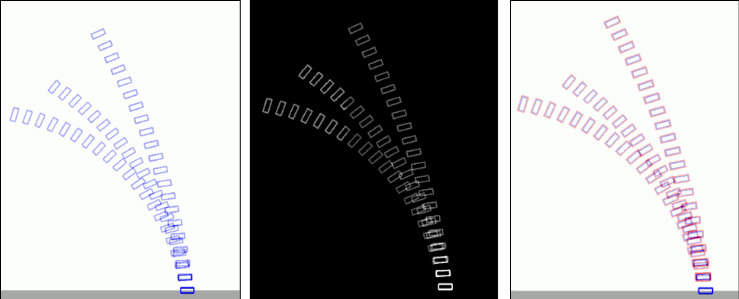
\includegraphics[scale=.35]{figures/cv_seq.png}}
% \caption{Image analysis pipeline to obtain the Cartesian pose of $N$ cross-sections, applied to a sequence of video frames. From left to right: 1) original image; 2) binarized image; 3) original image superimposed with the fitted rectangles.}
% \label{fig:pcsregression:cv_sequence}
% \end{figure}

\subsubsection{Evaluation metrics}
To evaluate the models quantitatively, we introduce position and orientation task space metrics. 
We use a Cartesian-space \gls{MAE} measuring the deviation of the estimated from the actual robot body shape, given by

\begin{equation}
\begin{split}
    % e_\mathrm{p}^{\mathrm{body}} =& \: \frac{1}{N T} \sum_{k=1}^T \sum_{i=1}^N \lVert \hat{p}_i(k) - p_i(k) \Vert_2,\\
    % e_{\theta}^{\mathrm{body}} =& \: \frac{1}{N T} \sum_{k=1}^T \sum_{i=1}^N | \hat{\theta}_i(k) - \theta_i(k) |,
     e_\mathrm{p}^{\mathrm{body}} = \sum_{k=1}^T \sum_{j=1}^N \frac{\lVert \hat{p}_j(k) - p_j(k) \Vert_2}{N T},
     \quad
    e_{\theta}^{\mathrm{body}} = \sum_{k=1}^T \sum_{j=1}^N \frac{| \hat{\theta}_j(k) - \theta_j(k) |}{N T},
\end{split}
\end{equation}
where 
% $\hat{p}_i(k) = \begin{bmatrix}
%     \hat{p}_{\mathrm{x},i}(k) & \hat{p}_{\mathrm{y},i}(k)
% \end{bmatrix}^\top \in \mathbb{R}^2$ 
$\hat{p}_i(k)$ and $\hat{\theta}_i(k) \in \mathbb{R}$ are the estimated position and orientation of point $i$ along the structure, respectively, while $p_i(k)$ and $\theta_i(k)$ are the ground-truth counterparts. These metrics give the average pose error across all $T$ frames of a trajectory and all $N$ cross-sections tracked along the robot, enabling a good evaluation of the kinematic model by capturing how well it represents the overall shape of the soft robot structure.

\begin{figure*}[ht]
    \centering
    \subfigure[2S PCS: Strain distances]{\includegraphics[width=0.49\textwidth,trim={5 5 5 5}]{pcsregression/figures/distance_plot_two_segments.pdf}\label{fig:pcsregression:results:kinematic_fusion:pcs_ns-2}}
    \subfigure[3S PCS: Strain distances]{\includegraphics[width=0.49\textwidth,trim={5 5 5 5}]{pcsregression/figures/distance_plot_three_segments.pdf}\label{fig:pcsregression:results:kinematic_fusion:pcs_ns-3}}\\
    \subfigure[1S PAC: Strain distances]{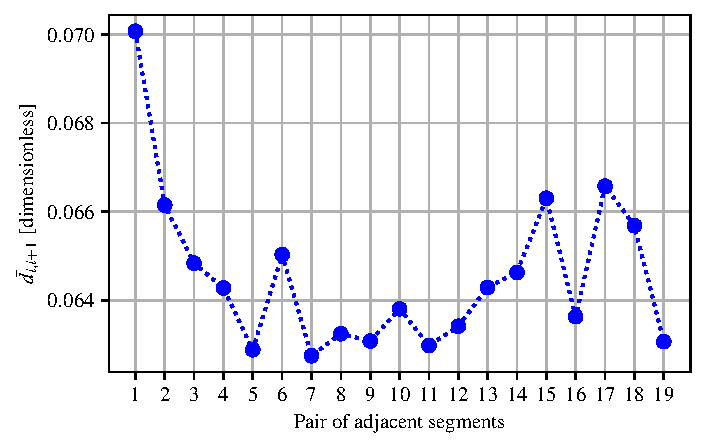
\includegraphics[width=0.46\textwidth,trim={5 5 5 5}]{pcsregression/figures/distance_plot_pac.pdf}\label{fig:pcsregression:distances_pac}}
    \subfigure[1S PAC: Kinematic Pareto Front]{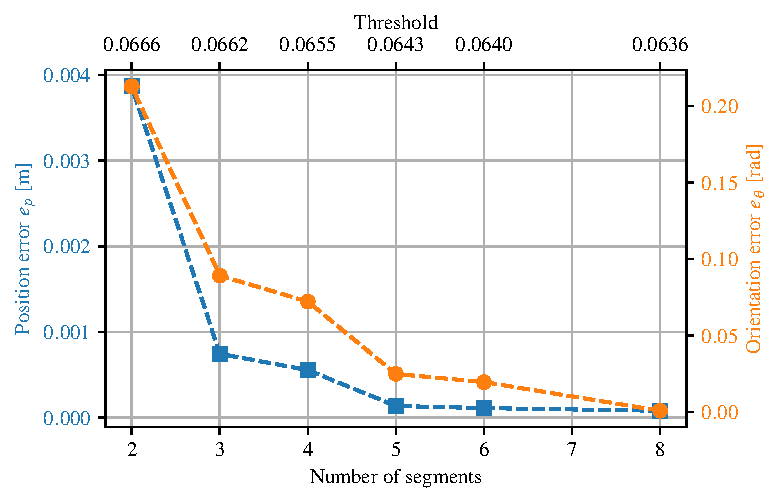
\includegraphics[width=0.50\textwidth,trim={5 5 5 5}]{pcsregression/figures/pareto_front_pac.pdf}\label{fig:pcsregression:pareto_front_pac}}
    \caption{
    Kinematic Fusion Results:
    \textbf{Panels (a) \& (b):} Average strain distances between pairs of adjacent segments for \emph{Cases 2 \& 3}. The poses of $20$ markers along the manipulators are tracked, resulting in $19$ pairs of segments to be evaluated for strain similarity. The threshold is represented by a dashed line, and the background shading marks the resulting segments (separate segments are shaded in different colors).
    \textbf{Panel (c):} Average strain distances between segments after the first iteration of the kinematic fusion algorithm for \emph{Case 6}. \textbf{Panel (d):} Pareto front that describes the trade-off between the DOF of the kinematic model (i.e., the number of segments) and the shape reconstruction error for \emph{Case 6}.
    The blue and orange lines represent the average kinematic body position error $e_\mathrm{p}^\mathrm{body}$ and the body orientation error $e_\theta^\mathrm{body}$, respectively.
    % Position ($\blacksquare$) and orientation ($\CIRCLE$) distributed errors as a function of the number of segments considered for the kinematic model in Case 6.
    The strain distance threshold $h$ that is used for separating segments is plotted on the upper x-axis.
    }\label{fig:pcsregression:results:kinematic_fusion}
\end{figure*}

In addition, we consider an end-effector Cartesian-space \gls{MAE} given by
\begin{equation}
    e_p^{\mathrm{ee}} = \frac{1}{ T} \sum_{k=1}^T \lVert \hat{p}_\mathrm{ee}(k) - p_\mathrm{ee}(k) \rVert_2,
    \quad
    e_{\theta}^{\mathrm{ee}}=\frac{1}{T} \sum_{k=1}^T | \hat{\theta}_\mathrm{ee}(k) - \theta_\mathrm{ee}(k) |,
\end{equation}
where $\hat{p}_\mathrm{ee}(k) = \hat{p}_{N}(k) \in \mathbb{R}^2$ and $\hat{\theta}_\mathrm{ee}(k) \in \mathbb{R}$ are the estimated end-effector position and orientation, respectively, with $p_\mathrm{ee}(k)$ and $\theta_\mathrm{ee}(k)$ being the ground-truth counterparts. 
This metric is particularly useful for assessing the obtained dynamic models with a control perspective, as the accuracy of the end-effector predictions is crucial for effective control in task space.
% For the kinematic model, once the final number of segments $m$ and their locations are determined, we retrieve for the test trajectory the configurations $\mathbf{q}_i(k)$ at each of the segments. Then, knowing the coordinate $s$ of each of the $N$ tracked points along the robot, the estimated positions and orientations are found using the forward kinematics in \eqref{eq:pcsregression:forward_kin_pcs}. For the dynamic model, after obtaining the final coefficients for the Lagrangian and damping effects, we can get the robot's equations of motion. Those are integrated with the initial conditions of the test trajectory to obtain the estimated configurations. The estimated positions and orientations are again found as above through forward kinematics.

\subsection{Kinematic Fusion Results}
\subsubsection{Cases 1, 2, and 3}
% The kinematic fusion procedure was first tested for three instances of the planar PCS simulator: a one-, two- and three-segment manipulators (Cases 1, 2 and 3). %The video processing step extracts the poses of the 20 cross-sections and a 20-segment kinematic model is initialized. 
Figs. \ref{fig:pcsregression:results:kinematic_fusion:pcs_ns-2} \& \ref{fig:pcsregression:results:kinematic_fusion:pcs_ns-3} presents the average strain distances between the adjacent segment pairs for \emph{Cases 2-3}, as the result of the first and final iteration of the kinematic fusion algorithm. 
The plots for Cases 2 and 3 reveal one and two peaks, respectively, revealing where we need to separate segments in the kinematic model.
% In contrast, the smaller magnitude of the distance metric in Case 1, when compared to the other cases, indicates that the entire robot can be represented by a single segment with constant strain. 
The strain distance threshold $h$ is a hyperparameter that trades off model complexity with model accuracy.
For common soft robots that exhibit a \gls{PCS}-like behavior, we recommend choosing $h$ such as that the segmented model exhibits isolated peaks in the strain distance metric, as visible in Fig.~\ref{fig:pcsregression:results:kinematic_fusion}.
The number of segments and respective lengths for the resulting models obtained with a threshold of $h=0.2$ are presented in the third column of Table \ref{tab:pcsregression:results_kin_reg_pcs}, and by comparing to the second column, it is easily visible that our algorithm almost perfectly identified the segment lengths. 
% Note that these models are final because, for Cases 2 and 3, the updated strain trajectories for the newly defined segments are no longer sufficiently similar for further merging. Also, for Case 1 no additional merging is possible since we already reached one single segment.
%
% The distributed task-space errors between the resulting models and the ground truth is also evaluated. Knowing the final number of segments and their lengths, we determine the configurations $\mathbf{q}_i(k)$. Then, using the forward kinematics in \eqref{eq:pcsregression:forward_kin_pcs}, we obtain the estimated positions and orientations for the 20 tracked points along the robot. The results for these three cases are summarized in the first three rows of Table \ref{tab:pcsregression:results_kin_reg_pcs}.
As a consequence of the correct identification of the number of segments and segment lengths, the identified kinematic model also accurately captures the shape of the robot with the position errors below \SI{0.2}{\percent} of the robots' length, as it can be seen from the body shape reconstruction errors stated in the first three rows of Table \ref{tab:pcsregression:results_kin_reg_pcs}.
We remark that the error can be further reduced by using a finer discretization of backbone pose markers (i.e., increasing $N$).
% The evaluation of the kinematic fusion algorithm for Cases 4 \& 5 is not necessary as it would give very similar results as reported for Cases 1 \& 2.

\begin{table}[htbp]
\centering
% \renewcommand{\arraystretch}{1.3} % Increase space between rows
\caption{Kinematic fusion results: The second and third columns contain the actual and estimated segment lengths, respectively. The Cartesian pose error between the actual and estimated backbone shape is stated in the third and fourth columns, respectively. \emph{Case 6} represents a one-segment \gls{PAC} soft robot of total length \SI{150}{mm} and can be, therefore, not be represented with a (one-segment) \gls{PCS} model.}
\label{tab:pcsregression:results_kin_reg_pcs}
\setlength\tabcolsep{3.0pt}
\begin{small}
    \begin{tabular}{ccccc}\toprule
    \textbf{Case} & \begin{tabular}[c]{@{}c@{}}\textbf{Actual segment}\\ \textbf{lengths} $\mathbf{L}$ \textbf{[mm]}\end{tabular} & \begin{tabular}[c]{@{}c@{}}\textbf{Estimated segment}\\ \textbf{lengths} $\mathbf{\hat{L}}$ \textbf{[mm]}\end{tabular} & $\mathbf{e_\mathrm{p}^{\mathrm{body}}}$ \textbf{[mm]} & $\mathbf{e_{\theta}^{\mathrm{body}}}$ \textbf{[rad]} \\ \midrule
    \textbf{1: 1S PCS} & $[100]$ & $[100]$ & $0.082$ & $6.38\times 10^{-3}$ \\
    \textbf{2: 2S PCS} & $[70, 100]$ & $[68, 102]$ & $0.240$ & $1.15\times 10^{-2}$               \\
    \textbf{3: 3S PCS} & $[50, 100, 60]$ & $[52.5, 94.5, 63.0]$ & $0.210$ & $9.67\times 10^{-3}$ \\
    \textbf{6: 1S PAC} & $[150]$ & $[7.5, 105.0, 37.5]$ & $0.746$ & $8.92\times 10^{-2}$  \\
    \bottomrule
    \end{tabular}
\end{small}
\end{table}

% The kinematic fusion was able to retrieve models that almost exactly match the manipulators used in the simulation. However, for Cases 2 and 3, the segments' lengths deviate slightly from the true ones (see second column of Table \ref{table:manipulator_params}). This is a consequence of the number of cross-sections tracked along the robots. Increasing this number would result in finer discretization and a closer approximation. Nonetheless, the position errors of the resulting models fall under 0.2\% of the robots' lengths.

\subsubsection{Case 6}
Even though the kinematics of many continuum soft robotic manipulators can be described by \gls{PCS}/\gls{PCC} kinematics, other continuum soft robots can only be described by piecewise constant models in the limit $N \to \infty$ as they exhibit polynomial curvature~\citep{della2019control, stella2022experimental} or even more generally \gls{GVS}~\citep{boyer2020dynamics}.
This is particularly the case when external or gravitational forces dominate the elastic and actuation forces~\citep{della2023model}.
In order to verify that our approach is also able to identify effective models in such situations, we test the kinematic fusion algorithm on the case of an affine curvature robot~\citep{stella2023piecewise} and plot the resulting average strain distances in Fig.~\ref{fig:pcsregression:distances_pac}.
Indeed, the strain distance plot no longer exhibits clear, isolated peaks (i.e., a single solution). Therefore, we formulate a Pareto front in Fig.~\ref{fig:pcsregression:pareto_front_pac} (by varying the strain distance threshold $h$) that describes the tradeoff between the number of \gls{PCS} segments (i.e., the \gls{DOF} of the kinematic model) and the shape reconstruction accuracy. Analyzing and exploiting this tradeoff allows the user to choose their \emph{sweetspot} between model complexity and performance.
In this case, we find that three segments represent a suitable compromise between model complexity and shape reconstruction accuracy, as it exhibits a position error of only \SI{0.5}{\percent} of the robot's length.

% We evaluate the robustness of the method with the PAC simulator, which no longer implements the constant bending assumption of the PCS model. The average strain distances for the initial 19 pairs of segments are presented in Fig. \ref{fig:pcsregression:distances_pac}.


% Contrary to the results for the previous test cases, the plot does not make clear the exact locations where to merge segments. In this situation, we could think of the threshold as a hyperparameter and evaluate the quality of the models resultant from different values of $h$. Figure \ref{fig:pcsregression:pareto_front_pac} shows the position and orientation errors as a function of the obtained number of segments, for several values of threshold. The choice for the final kinematic model depends on how the user wants to balance model complexity and shape reconstruction accuracy. For this case, we choose as the final model the one that maximizes the decrease in error over an increase in complexity (i.e., number of segments), which corresponds to the model with three segments. We can see that the 3-segment model exhibits a distributed position error of 0.5\% of the robot's length, which verifies that this kinematic parametrization is suitable to approximate the robot's behaviour.

% \begin{figure}[htbp]
%     \centering
%     \subfloat[Position error\label{1a}]{%
%       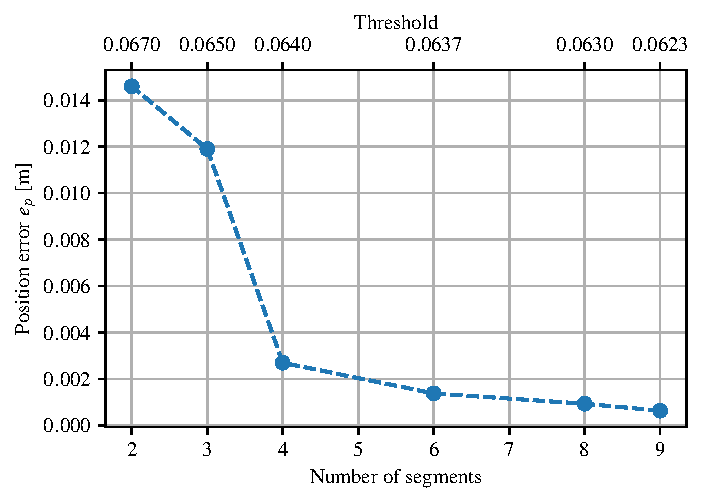
\includegraphics[width=0.8\linewidth]{pcsregression/figures/pareto_front_pac_pos.pdf}}
%     \\
%     \subfloat[Orientation error\label{1b}]{%
%        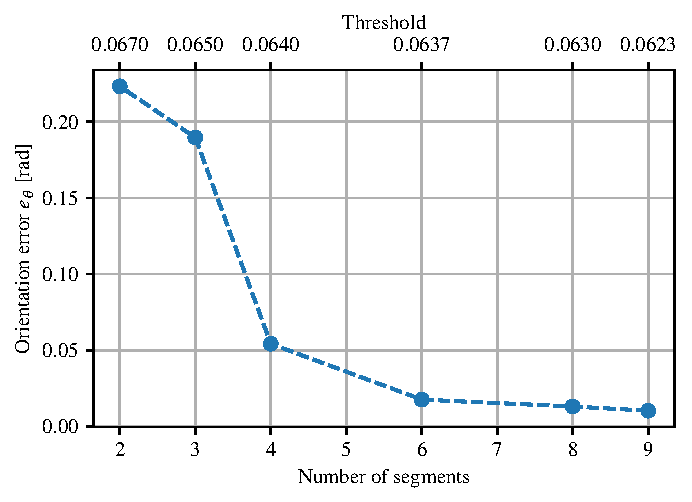
\includegraphics[width=0.8\linewidth]{pcsregression/figures/pareto_front_pac_ori.pdf}}
%        %\\

%     \caption{Average strain distances between pairs of adjacent segments for tasks generated using the PCS simulator. The poses of 20 cross-sections along the manipulators are tracked, resulting in 19 pairs of segments to be evaluated for strain similarity.}
%     \label{fig:pcsregression:pareto_front_pac}
% \end{figure}

% This 4-segment model was evaluated on the test trajectory and the task space errors are presented in the final row of Table \ref{table:results_kin_reg_pcs}. The positional error corresponds to 4\% of the robot's length, which verifies that this kinematic parametrization is suitable to approximate the robot's behavior.

\subsection{Dynamic Model Identification Results}

\subsubsection{Verification of Dynamical Regression}
We verify the dynamical regression algorithm on one and two-segment \gls{PCS} robots (i.e., Cases 1 \& 2), both with and without measurement noise.
After regressing the dynamic parameters on the training set, we perform a rollout on the test set and compare the resulting predicted trajectory with the ground truth.
To confirm that the dynamic regression is also effective when applied to real-world data, we apply in some experiments Gaussian noise that mirrors measurement noise as we would encounter it for motion capture data, computer vision detection errors, etc. to the poses included in the training set (i.e., $\Tilde{\chi} = \chi + \mathcal{N}(0, \sigma_\mathrm{n}))$.
For \emph{Case 1}, we sample the noise from a normal distribution with standard deviations \SI{0.5}{mm} and \SI{1}{\degree} for the position and orientation measurements, respectively.
Analog, we define the standard deviation of the noise for \emph{Case 2} as \SI{0.1}{mm} and \SI{0.5}{\degree}.

The results are reported in Tab.~\ref{tab:pcsregression:dyn_results} (top four rows), and the rollouts of Cases 1 \& 2 are included in Figs.~\ref{fig:pcsregression:predict_ns-1}-\ref{fig:pcsregression:predict_ns-2}. We also present a sequence of stills of the rollout of \emph{Case 2} in Fig.~\ref{fig:pcsregression:still_seq}.
We conclude that even though the dynamical parameters are regressed on only \SI{4}{s} of robot motion data, the dynamical predictions are extremely accurate on the long horizon of \SI{7}{s} (most control algorithms such as \gls{MPC} operate on a much smaller horizon). The position error for the experiments not involving noise stays below \SI{5}{\percent} in both cases.
When noise is present in the training data, the position error is roughly tripled. Still, we observe that the error is mostly related to the transient terms and the model converges during the slower sequences of the trajectory to the ground truth. Most importantly, the learned model, even when trained on noisy data, remains stable, as shown in Fig.~\ref{fig:pcsregression:predict_ns-2}.

\subsubsection{Verification of Strain Sparsification}
Next, we verify that the strain sparsification algorithm can detect and eliminate strains that do not have a significant effect on the dynamics and can be, therefore, neglected to reduce the model complexity.
For this purpose, we apply the integrated \emph{Dynamic Regression and Strain Sparsification} algorithm to \emph{Cases 4 \& 5}, which exhibit no shear strain and no axial strain (\nth{1}-segment) \& no shear strain (\nth{2}-segment), respectively.
We define the maximum elastic and shear modulus as $E^\mathrm{max} = \SI{100}{MPa}$ which leads to the stiffness thresholds for each segment $K_j^\mathrm{max} = \mathrm{diag}(\SI{12.6}{Nm^2}, \SI{168}{N}, \SI{126}{kN})$.
For example, in \emph{Case 4}, after determining the dynamic parameters during the first iteration, the algorithm detects that the estimated shear stiffness $\hat{K}_\mathrm{sh} = \SI{1200}{N} > K_\mathrm{sh}^\mathrm{max} = \SI{168}{N}$. Therefore, the shear strain is eliminated from the dynamic model, and the dynamic parameters are newly regressed during the next iteration.
Similarly, the algorithm correctly neglects the axial strain for the \nth{1} segment and the shear strain for the \nth{2} segment of \emph{Case 5}.
We visualize the test set rollouts for \emph{Cases 4 \& 5} in Fig.~\ref{fig:pcsregression:results:strain_sparsification} and report the error metrics in the last three rows of Tab.~\ref{tab:pcsregression:dyn_results}.
The results show that in \emph{Case 4}, the model without shear even exhibits a slightly smaller position error than the model that includes all strains. A possible explanation could be that with the Lagrangian being parametrized by fewer basis functions, the coefficients for the remaining strains can be more accurately regressed.
If we compare \emph{Case 2} and \emph{Case 5} (both two-segment \gls{PCS} robots), \emph{Case 5} exhibits significantly increased position and orientation errors. Still, we notice that the model predictions are usable, in particular for shorter horizons.

% We now present and discuss the results of the dynamic model identification procedure. The procedure is the same across all the tested manipulators. From the kinematic fusion step, we retrieve the kinematic model (with generic $m$-segments) and the respective configurations $\mathbf{q}(k) \in \mathbb{R}^{3m}$ for each of the 4000 time steps captured throughout the eight generated trajectories. The velocity $\dot{\mathbf{q}}(k)$ and acceleration $\ddot{\mathbf{q}}(k)$, also required for the regression, are numerically approximated using the Savitzky-Golay filter \citep{savitzky_smoothing_1964}, with a window length of 25 and a third-order polynomial. We gather the basis functions of the $m$-segment PCS Lagrangian (considering all three strains per segment) and initialize the diagonal damping matrix $\mathbf{D} \in \mathbb{R}^{3m\times 3m}$ to be also identified. After running the least-squares regression and strain sparsification iteratively, we compute the Euler-Lagrange equations with the obtained model and retrieve the robot's equations of motion. We then simulate the model for the sinusoidal validation trajectory, using a Tsitouras 5(4) integrator \citep{tsitouras_rungekutta_2011} and a time-step of 0.1 $\mathrm{ms}$.
% \subsubsection{Case 1}
% The Lagrangian of a one-segment PCS manipulator contains 51 basis functions. To those, we also add the 3 damping terms, yielding 54 coefficients to be identified.

\begin{table}[htbp]
\centering
% \renewcommand{\arraystretch}{1.2}
\caption{Dynamic regression results: End-effector position and orientation errors $\mathbf{e_\mathrm{p}^{\mathrm{ee}}}, \mathbf{e_{\theta}^{\mathrm{ee}}}$ for the obtained dynamic models evaluated on the \SI{7}{s} sinusoidal test set trajectory. In some cases, we add artificial measurement noise to the training data. For \emph{Case 4}, we present two variants of the learned model: in the first instance, we report the performance of a model that neglects strains as suggested by the dynamic sparsification algorithm. For completeness, we furthermore also state the performance of a model that considers all strains. In \emph{Case 5}, the \nth{1} segment only exhibits bending and shear strains (i.e, no axial strain), and the \nth{2} segment only exhibits bending and axial strains (i.e., no shear strain)}
\label{tab:pcsregression:dyn_results}
\setlength\tabcolsep{2pt}
\begin{small}
\begin{tabular}{c c c c c }
    \toprule
    \textbf{Case} & \textbf{Meas. Noise} & \textbf{Model Strains}     & $\mathbf{e_\mathrm{p}^{\mathrm{ee}}}$ \textbf{[mm]} & $\mathbf{e_{\theta}^{\mathrm{ee}}}$ \textbf{[rad]} \\
    \midrule
    1: 1S PCS & \xmark                     & All                & $4.89$    & $0.113$             \\ 
    1: 1S PCS & \cmark                        & All                & $13.7$    & $0.307$             \\ 
    \midrule
    2: 2S PCS & \xmark                     & All                & $5.22$    & $0.138$             \\
    2: 2S PCS & \cmark                        & All                & $16.8$    & $0.135$             \\ 
    \midrule
    4: 1S PCS H-SH & \xmark & No shear                     & $4.57$    & $0.099$                                 \\ 
    4: 1S PCS H-SH & \xmark & All                & $5.14$    & $0.116$ \\
    \midrule
    5: 2S PCS H-AX/SH & \xmark & (\cmark, \cmark, \xmark, \cmark, \xmark, \cmark) & $17.9$ & $0.305$\\
    \bottomrule
\end{tabular}
\end{small}
\end{table}

% After performing the least-squares regression, we inspect the estimated stiffness and compare it to the maximum defined stiffness. We choose $E^{\text{max}}=100 \,\mathrm{MPa}$ and $G^{\text{max}}=0.1 \,\mathrm{MPa}$, which are in line with the range of soft materials typically used \citep{gariya_review_2021}. For the cross-section area $A_c$ and second moment of inertia $I_c$, we assumed a constant circular cross-section along the segment, with the same radius defined in the simulator. With the above parameters, the maximum stiffness is
% \begin{equation}\label{eq:pcsregression:max_stiffness}
%     \begin{aligned}
%         K^{\text{max}} &=\mathrm{diag} \begin{bmatrix}
%         k_{\text{be}}^{\text{max}} & k_{\text{sh}}^{\text{max}} & k_{\text{ax}}^{\text{max}}   
%         \end{bmatrix} \\
%         &= \mathrm{diag}\begin{bmatrix}
%             1.26\times 10^1 & 1.68 \times 10^2 & 1.26\times10^5
%         \end{bmatrix} \,.
%     \end{aligned}
% \end{equation}

% The estimated stiffness obtained from the regression is
% \begin{align}
%     \hat{K} = \mathrm{diag} \begin{bmatrix}
%     1.20\times 10^{-3} & 1.55 \times 10^0 & 1.14\times10^1 
% \end{bmatrix}\,.
% \end{align}

% Since all values are below the maximum, no strains will be neglected and the dynamic model is final.

% To evaluate the robustness of the method, we also corrupted the videos by adding zero-mean Gaussian noise to the position and orientation of each of the 20 cross-sections along the robot. Specifically, noise with a standard deviation of $5 \times 10^{-4} \, \mathrm{m}$ was added to both the $x$- and $y$-position measurements, while a standard deviation of $1\, \mathrm{deg}$ was applied to the orientation. Figure \ref{fig:pcsregression:predict_ns-1} shows the comparison between the models trained with and without noise. 

\begin{figure*}[htbp]
    \centering
    \subfigure[Configurations]{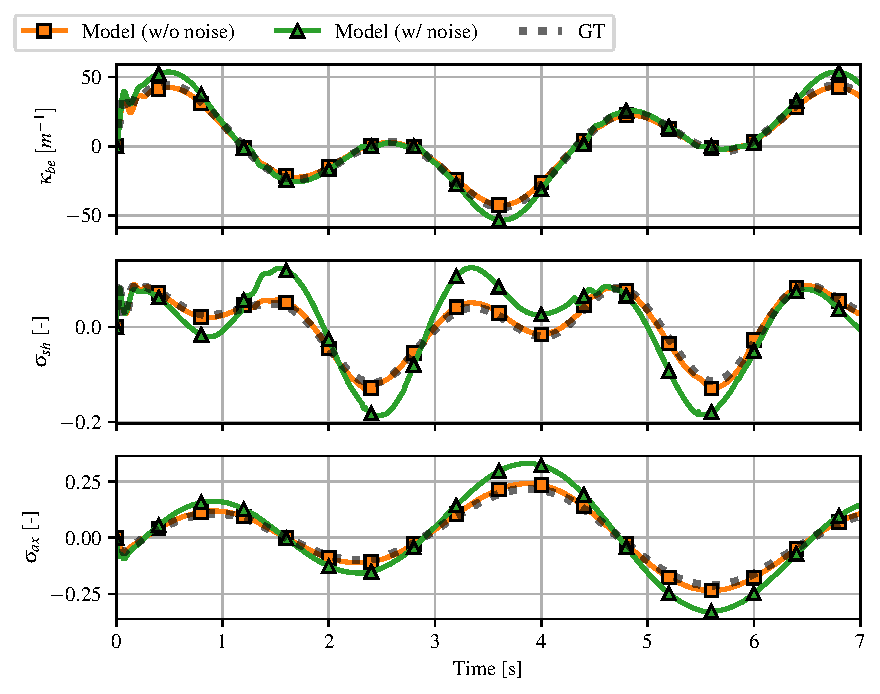
\includegraphics[width=0.49\linewidth]{pcsregression/figures/pcs_ns-1/ns-1_configuration_plots.pdf}\label{fig:pcsregression:predict_ns-1_subfig-1}}
    \subfigure[End-effector pose]{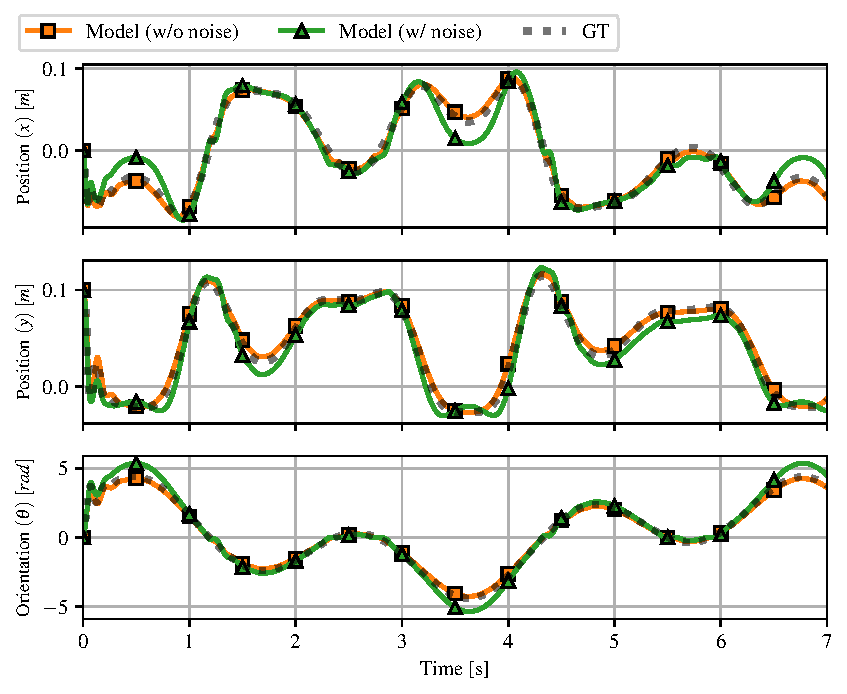
\includegraphics[width=0.47\linewidth]{pcsregression/figures/pcs_ns-1/ns-1_ee_comparison_plots.pdf}\label{fig:pcsregression:predict_ns-1_subfig-2}}

    \caption{Verification of the model obtained for Case 1 on a sinusoidal trajectory. The dotted line denotes the ground-truth (GT) trajectory, while the green and orange lines correspond to the models trained with and without noise, respectively.}
    \label{fig:pcsregression:predict_ns-1}
\end{figure*}

% The task-space error analysis, reported on Table \ref{tab:pcsregression:dyn_results}, show that the model trained without noise is able to give very accurate predictions, with the end-effector position error being under $5\%$ of the robot's length. The model trained from noisy data can still provide reasonable predictions, even though the position error increases to $1.37\, \mathrm{cm}$ and the orientation error rises to $0.3\, \mathrm{rad}$. 

% \begin{table*}[htbp]
% \centering
% \renewcommand{\arraystretch}{1.5}
% \caption{Error metrics for Cases 1, 2, and 4. Distributed task-space errors and end-effector errors are reported for both position and orientation. Cases 1 and 2 include results with and without added noise during training.}
% \label{tab:pcsregression:dyn_results}
% \begin{tabular}{|>{\centering\arraybackslash}p{1.5cm}|c|c|c|c|c|}
% \hline
% \multirow{2}{*}{\textbf{Case}} & \multirow{2}{*}{\textbf{Noise}} & \multicolumn{2}{c|}{\textbf{Distributed Errors}} & \multicolumn{2}{c|}{\textbf{End-Effector Errors}} \\ \cline{3-6} 
%                                 &                                   & $e_p^{\mathrm{body}}$ [m] & $e_{\theta}^{\mathrm{body}}$ [rad] & $e_p^{\mathrm{ee}}$ [m] & $e_{\theta}^{\mathrm{ee}}$ [rad] \\ \hline
% \textbf{1}                      & Without noise                     & $1.96\times 10^{-3}$      & $5.92\times 10^{-2}$               & $4.89\times 10^{-3}$    & $1.13\times 10^{-1}$             \\ \cline{2-6}
%                                 & With noise                        & $6.64\times 10^{-3}$      & $1.61\times 10^{-1}$               & $1.37\times 10^{-2}$    & $3.07\times 10^{-1}$             \\ \hline
% \textbf{2}                      & Without noise                     & $3.07\times 10^{-3}$      & $4.07\times 10^{-2}$               & $5.22\times 10^{-3}$    & $1.38\times 10^{-1}$             \\ \cline{2-6}
%                                 & With noise                        & $7.06\times 10^{-3}$      & $1.04\times 10^{-1}$               & $1.68\times 10^{-2}$    & $1.35\times 10^{-1}$             \\ \hline
% \textbf{4}                      & -                                 & $4.12\times 10^{-4}$      & $1.89\times 10^{-2}$               & $4.50\times 10^{-4}$    & $1.95\times 10^{-2}$             \\ \hline
% \end{tabular}
% \end{table*}

% \begin{table}[h]
% \centering
% \caption{Task-space errors for the obtained dynamic models in Cases 1 and 4.}
% \label{tab:pcsregression:dyn_results}
% \begin{tabular}{ccc}
% \hline
% Case & $e_p\,[\mathrm{m}]$  & $e_{\theta}\,[\mathrm{rad}]$ \\ \hline
% \textbf{1}    & $1.39\times 10^{-3}$ & $3.07 \times 10^{-2}$    \\ \hline
% \textbf{4}    & $4.88\times 10^{-4}$ & $1.40 \times 10^{-2}$    \\ \hline
% \end{tabular}
% \end{table}

% An actual visualization of the trajectory also allows us to see that the end-effector error tends to increase after the robot crosses its straight configuration. Figure \ref{fig:pcsregression:still_seq} shows a sequence of stills from the trajectory where this behaviour is noticeable. A possible reason for this is that, in the simulator used for generating the data, a small $\varepsilon$ is added to the bending strain to avoid numerical instabilities due to divisions by zero.  This introduces a minor nonlinearity that is not accounted for in the system's Lagrangian, and consequently, it is not captured by the learned model.

% \subsubsection{Case 2}
% The Lagrangian of a two-segment PCS manipulator has 438 basis functions. In total, that leads to 444 coefficients to be estimated (438 plus 6 damping terms). Using also $E^{\text{max}}=100 \,\mathrm{MPa}$ and $G^{\text{max}}= \SI{0.1}{MPa}$, and assuming the same cross-section radius for both segments of $0.02\, \mathrm{m}$, the maximum stiffness is 
% \begin{equation}
% \begin{aligned}
% K^{\text{max}} &= \text{diag} \left[ 
%     k_{\text{be,1}}^{\text{max}} \,\,\,\, k_{\text{sh,1}}^{\text{max}} \,\,\,\,
%     k_{\text{ax,1}}^{\text{max}} \,\,\,\,
%     k_{\text{be,2}}^{\text{max}} \,\,\,\, k_{\text{sh,2}}^{\text{max}} \,\,\,\, k_{\text{ax,2}}^{\text{max}} \right] \\
% &= \text{diag} \left[ 1.26 \times 10^{1} \,\,\,\, 1.68 \times 10^{2} \,\,\,\, 1.26 \times 10^{5} \right. \\
% &\phantom{= \text{diag} \,} \left. 1.26 \times 10^{1} \,\,\,\,  1.68 \times 10^{2} \,\,\,\, 1.26 \times 10^{5} \right]\,.
% \end{aligned}
% \end{equation}
%  After the least-squares regression, the estimated stiffness coefficients are
% \begin{equation}
% \begin{aligned}
% \hat{K} &= \text{diag} \left[ 1.07 \times 10^{-3} \,\,\,\, 1.31 \times 10^{0} \,\,\,\, 1.09 \times 10^{1} \right. \\
% &\quad\quad\quad \left. 1.11 \times 10^{-3} \,\,\,\, 4.28\times 10^0 \,\,\,\, 9.60\times 10^0 \right]\,,
% \end{aligned}
% \end{equation}
% which means that no strains are neglected since all the values are smaller than the corresponding maximum.

% As with the one-segment case, we also corrupted the videos by adding measurement noise (through a zero-mean Gaussian distribution) to the position and orientation of the cross-sections split along the robot. However, in this case, the method could only tolerate noise with a standard deviation of $1 \times 10^{-4} \,\mathrm{m}$ for the position and $0.5\, \mathrm{deg}$ for the orientation. Training the models with data corrupted by higher noise levels caused the prediction results to diverge, as the estimated coefficients produced a mass matrix that was not positive definite, a condition necessary to ensure the stability of the dynamics. Figure \ref{fig:pcsregression:predict_ns-2} reports the comparison between the models trained both with and without noise for the sinusoidal trajectory used as validation.

\begin{figure}[htbp]
    \centering
    % First subfigure
    \subfigure[Configurations]{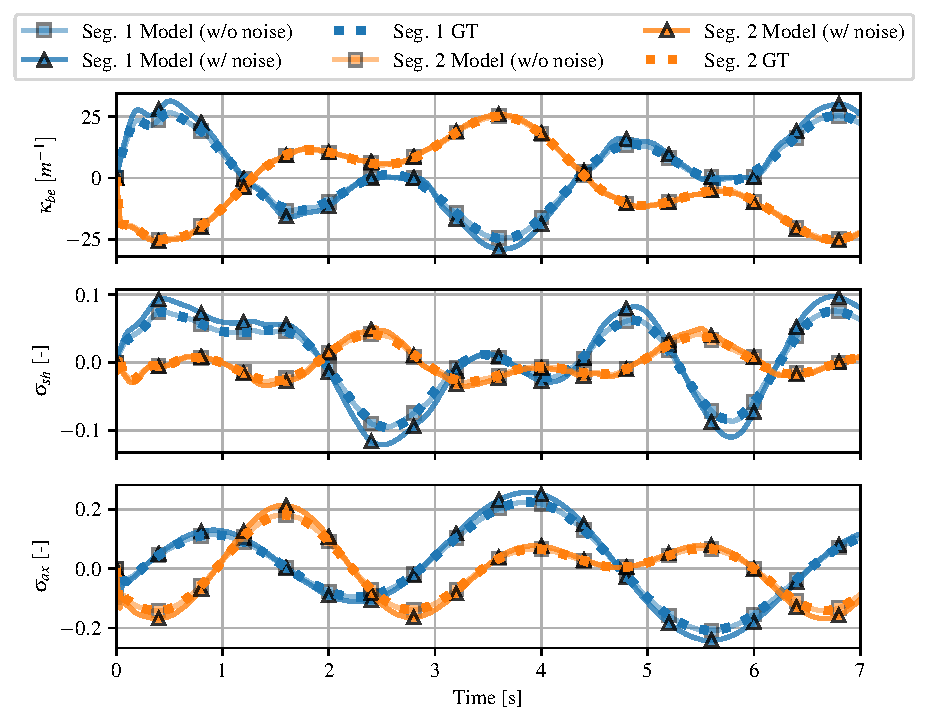
\includegraphics[width=0.49\textwidth, trim={5 5 5 5}]{pcsregression/figures/pcs_ns-2/ns-2_configuration_plots.pdf}\label{fig:pcsregression:predict_ns-2:subfig-1}}
    % Second subfigure
    \subfigure[End-effector pose]{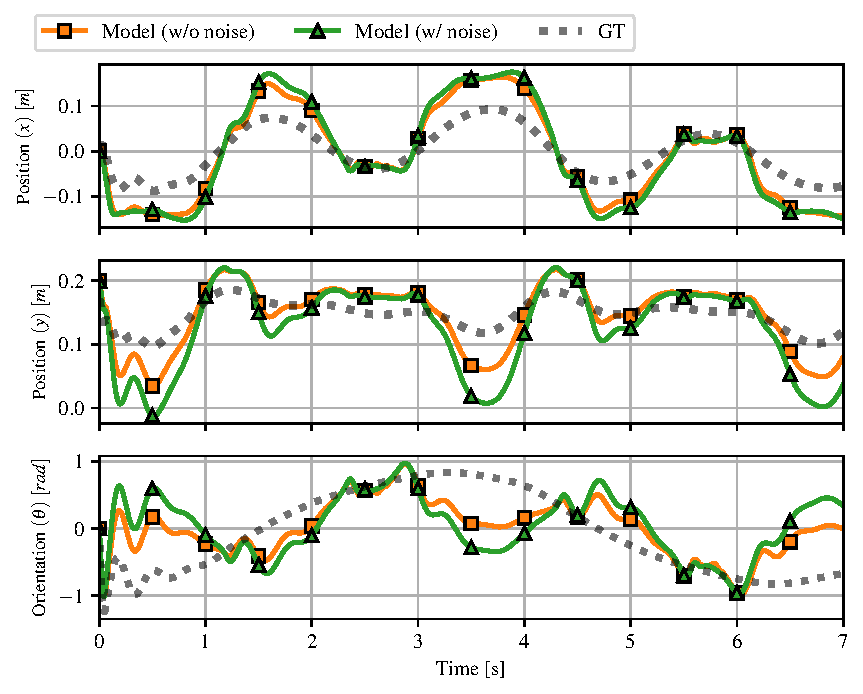
\includegraphics[width=0.47\textwidth, trim={5 5 5 5}]{pcsregression/figures/pcs_ns-2/ns-2_ee_comparison_plots.pdf} \label{fig:pcsregression:predict_ns-2:subfig-2}}

    \caption{Verification of the dynamical model with noise for a two-segment PCS soft robot (\emph{Case 2}). The dotted lines denote the ground-truth (GT) trajectory. For the configuration plot, blue lines refer to the first segment, while orange lines are associated with the second segment. For the end-effector pose plot, the orange and green lines mark the models trained with and without noise, respectively.}
    \label{fig:pcsregression:predict_ns-2}
\end{figure}
% \begin{figure}[htbp]
%     \centering
%     % First subfigure
%     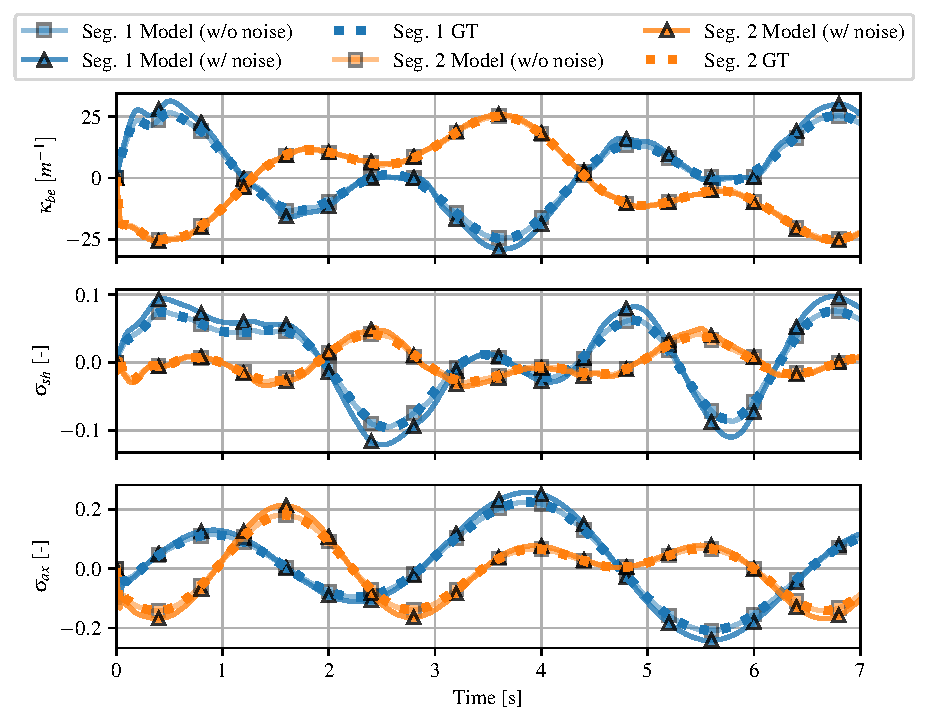
\includegraphics[width=0.8\columnwidth, trim={5 5 5 5}]{pcsregression/figures/pcs_ns-2/ns-2_configuration_plots.pdf}\label{fig:pcsregression:predict_ns-2_subfig-1}

%     \caption{Verification of the dynamical model with noise for a two-segment PCS soft robot (\emph{Case 2}). The dotted lines denote the ground-truth (GT) trajectory. The blue lines refer to the first segment, while the orange lines are associated with the second segment. % For the end-effector pose plot, the orange and green lines mark the models trained with and without noise, respectively.
%     }
%     \label{fig:pcsregression:predict_ns-2}
% \end{figure}

\begin{figure*}[ht]
    \centering
    \subfigure[$t=\SI{0.0}{s}$]{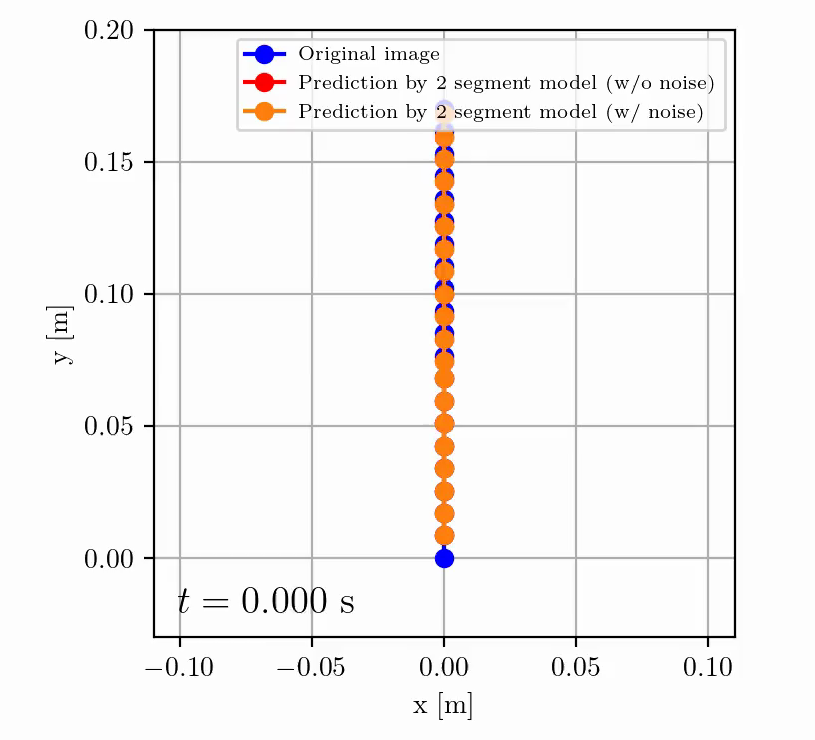
\includegraphics[width=0.320\textwidth,trim={5 5 5 5}]{pcsregression/figures/pcs_ns-2/sequence_of_stills/ns-2_task_space_animation_noise_comp_0.00.png}}
    \subfigure[$t=\SI{1.4}{s}$]{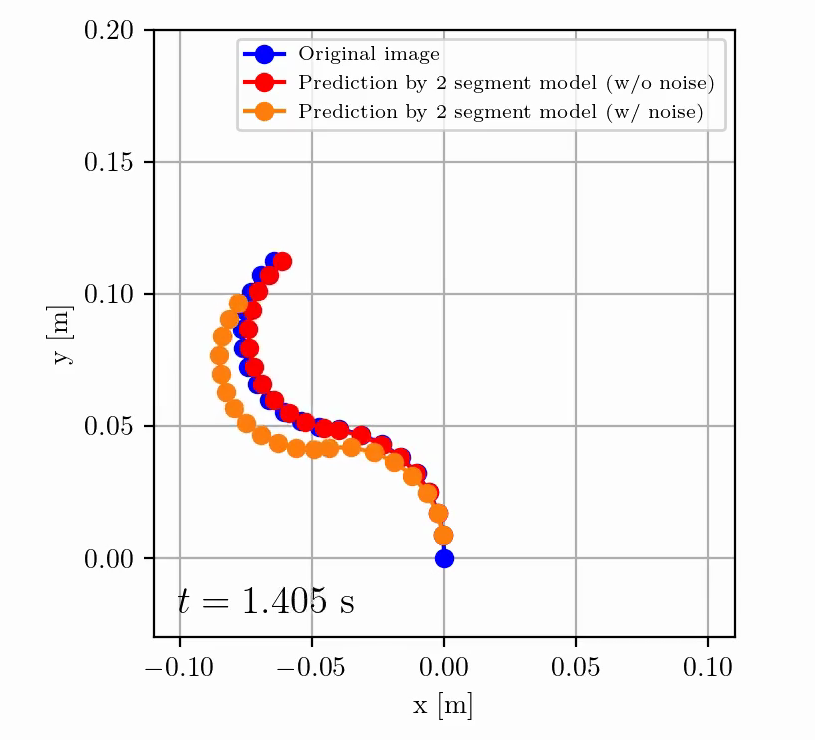
\includegraphics[width=0.320\textwidth,trim={5 5 5 5}]{pcsregression/figures/pcs_ns-2/sequence_of_stills/ns-2_task_space_animation_noise_comp_1.40.png}}
    \subfigure[$t=\SI{2.8}{s}$]{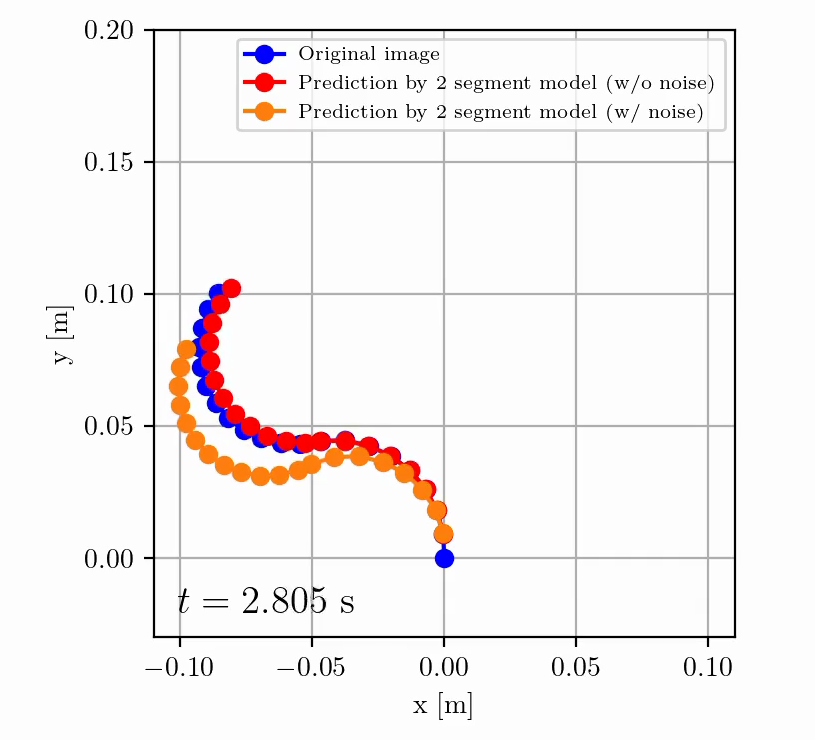
\includegraphics[width=0.320\textwidth,trim={5 5 5 5}]{pcsregression/figures/pcs_ns-2/sequence_of_stills/ns-2_task_space_animation_noise_comp_2.80.png}}\\
    \subfigure[$t=\SI{4.2}{s}$]{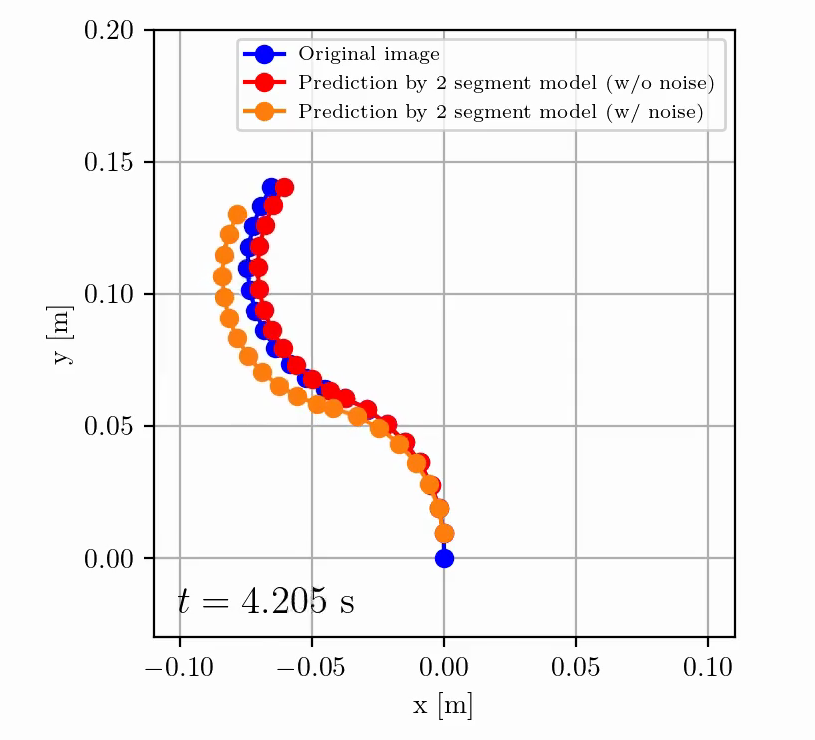
\includegraphics[width=0.320\textwidth,trim={5 5 5 5}]{pcsregression/figures/pcs_ns-2/sequence_of_stills/ns-2_task_space_animation_noise_comp_4.21.png}}
    \subfigure[$t=\SI{5.6}{s}$]{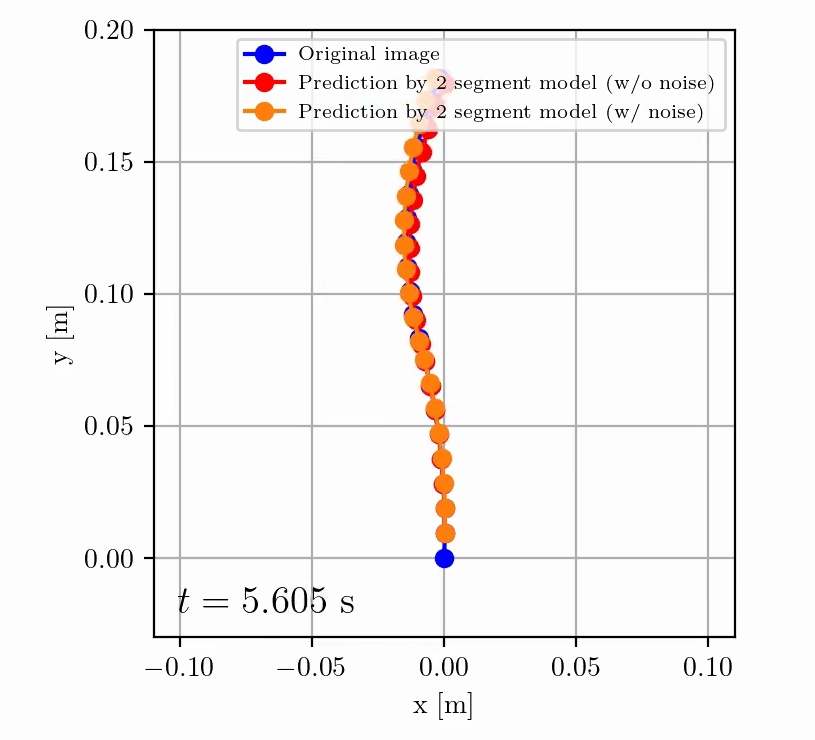
\includegraphics[width=0.320\textwidth,trim={5 5 5 5}]{pcsregression/figures/pcs_ns-2/sequence_of_stills/ns-2_task_space_animation_noise_comp_5.61.png}}
    \subfigure[$t=\SI{7.0}{s}$]{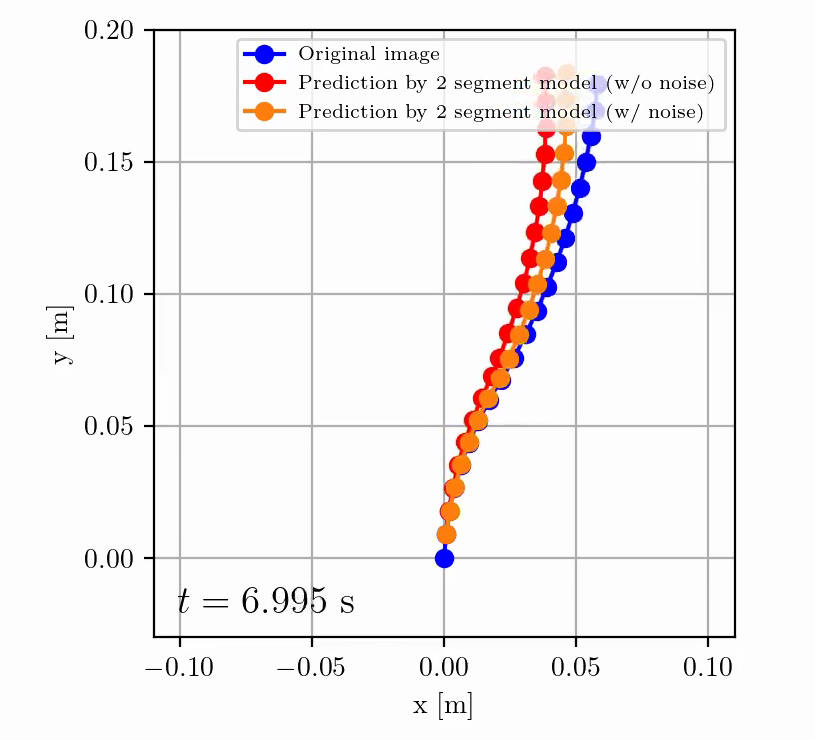
\includegraphics[width=0.320\textwidth,trim={5 5 5 5}]{pcsregression/figures/pcs_ns-2/sequence_of_stills/ns-2_task_space_animation_noise_comp_7.00.png}}
    \caption{Sequence of stills for the test rollout of the regressed dynamic model trained on the two-segment \gls{PCS} dataset (\emph{Case 2}). The blue and red dots represent the ground truth and estimated shape of the soft robot, respectively. The orange line represents the shape estimated by a model trained on a training set with added measurement noise.}\label{fig:pcsregression:still_seq}
\end{figure*}
% \begin{figure*}[htbp]
% \centerline{\includegraphics[width=\textwidth]{pcsregression/figures/sequence_stills.pdf}}
% \caption{Sequence of stills for the validation trajectory of Case 1, with the model trained without noisy data. The blue dots represent the actual position of the soft robot, while the red dots mark the position of the learned dynamic model.}
% \label{fig:pcsregression:still_seq}
% \end{figure*}

% The model trained without noise reports great accuracy, with an end-effector position error of $5.22\, \mathrm{mm}$ (3\% of the robot's length) and an orientation error of $0.14\,\mathrm{rad}$. An expected performance degradation is noticed for the model trained with noisy data, particularly for the end-effector position, which sees the error increase to $1.68\, \mathrm{cm}$. This raises some considerations for implementations in real-world scenarios where measurement noise is inevitable. Thus, while the model still gives reasonable predictions to moderate levels of noise, applying noise filtering techniques during the kinematic fusion process (where the measured task-space poses are converted into configurations) could help improve the robustness of the method to higher levels of noise.
% \subsubsection{Case 4}
% To evaluate the strain sparsification step in the dynamic regression, we used a one-segment PCS manipulator similar to Case 1, but with the shear strain stiffness set to a high value to simulate a scenario with minimal shear displacement.

% After running the regression, the obtained estimated stiffness was
% \begin{align}
%     \hat{K} = \mathrm{diag} \begin{bmatrix}
%     1.07\times 10^{-3} & 1.20 \times 10^3 & 1.16\times10^1 
% \end{bmatrix}\,.
% \end{align}
% Comparing the values with the maximum stiffness in \eqref{eq:pcsregression:max_stiffness}, the second entry, correspondent to the shear stiffness, is above the maximum value. Given this, the shear strain is neglected from the configuration vector and we update the Lagrangian basis functions through \eqref{eq:pcsregression:update_basis_fcns}, which results in a reduction from 51 to 27 basis functions. The Euler-Lagrange basis functions are also updated through \eqref{eq:pcsregression:update_basis_fcns_euler_lagrange}. The regression is again performed to estimate the 29 coefficients (27 plus the remaining 2 damping terms). In this case, the estimated stiffness is
% \begin{align}
%     \hat{K} =\mathrm{diag} \begin{bmatrix}
%         \hat{k}_{\text{be}} & \hat{k}_{\text{ax}}   
%         \end{bmatrix} = \mathrm{diag}\begin{bmatrix}
%             1.21\times 10^{-3} & 1.17 \times 10^1 
%         \end{bmatrix} \,,
% \end{align}
% which no longer requires additional sparsification.
% Figure \ref{fig:pcsregression:predict_ns-1_high_shear} shows the results for rolling out this dynamic model over the sinusoidal trajectory. To observe the impact of neglecting the shear strain, we additionally plot the end-effector pose for the case where shear was still considered. The end-effector errors for this comparison are also reported in the last two rows of Table \ref{tab:pcsregression:dyn_results}.


% \begin{figure}[htbp]
%     \centering
%     % First subfigure
%     \subfigure[Configurations]{\includegraphics[width=0.46\textwidth]{pcsregression/figures/ns-1_configuration_plots_high_shear.pdf}\label{fig:pcsregression:predict_ns-1_high_shear_subfig-1}}
%     % Second subfigure
%     \subfigure[End-effector pose]{\includegraphics[width=0.465\textwidth]{pcsregression/figures/ns-1_ee_comparison_plots_shear_vs_no_shear.pdf}\label{fig:pcsregression:predict_ns-1_high_shear_subfig-2}}

%     \caption{Verification of the model obtained for Case 4 on a sinusoidal trajectory. The dotted line denotes the ground-truth trajectory, while the green and orange lines correspond to the models trained with and without noise, respectively.}
%     \label{fig:pcsregression:predict_ns-1_high_shear}
% \end{figure}

\begin{figure}[ht]
    \centering
    % First subfigure
    \subfigure[Case 4: Configurations]{\includegraphics[width=0.47\linewidth, trim={5 5 5 5}]{pcsregression/figures/pcs_ns-1_high_shear_stiffness/ns-1_configuration_plots_high_shear.pdf}\label{fig:pcsregression:predict_ns-1_high_shear_subfig-1}}
    % Second subfigure
    \subfigure[Case 4: End-effector pose]{\includegraphics[width=0.49\linewidth, trim={5 5 5 5}]{pcsregression/figures/pcs_ns-1_high_shear_stiffness/ns-1_ee_comparison_plots_shear_vs_no_shear.pdf}\label{fig:pcsregression:predict_ns-1_high_shear_subfig-2}}\\
    \subfigure[Case 5: Configurations]{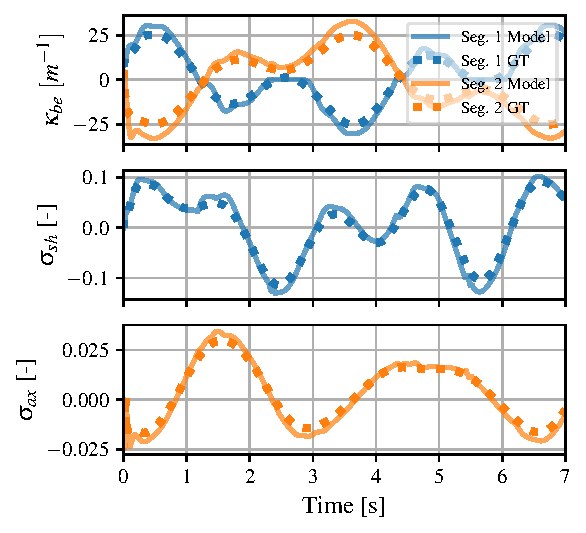
\includegraphics[width=0.49\linewidth, trim={5 5 5 5}]{pcsregression/figures/pcs_ns-2_high_stiffness/ns-2_configuration_plots.pdf}\label{fig:pcsregression:predict_ns-2_high_stiffness_subfig-1}}
    \subfigure[Case 5: End-effector pose]{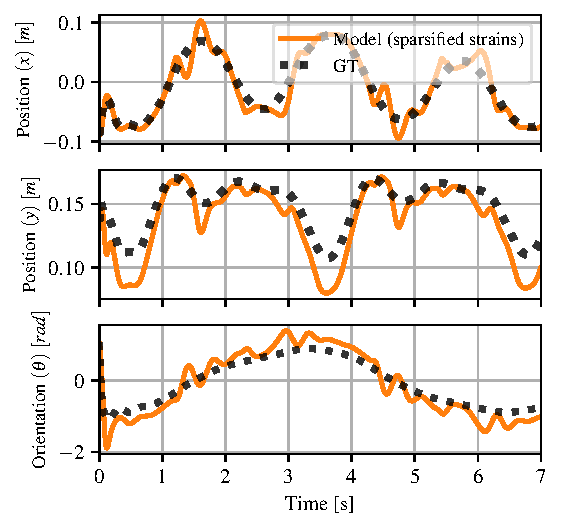
\includegraphics[width=0.47\linewidth, trim={5 5 5 5}]{pcsregression/figures/pcs_ns-2_high_stiffness/ns-2_ee_comparison_plots.pdf}\label{fig:pcsregression:predict_ns-2_high_stiffness_subfig-2}}

    \caption{Verification of the strain sparsification algorithm on a one-segment \gls{PCS} robot with shear modulus (\emph{Case 4}) and on a two-segment \gls{PCS} robot where the \nth{1} segment exhibits high axial stiffness and the second segment high shear stiffness. We roll out both the ground truth (dotted line) and the learned (solid line) model dynamics from the same initial condition and for a given sinusoidal actuation sequence.  Verification of the model obtained for Case 4 on a sinusoidal trajectory. The dotted line denotes the ground-truth trajectory, while the green and orange lines correspond to the models trained with and without noise, respectively.
    % For \emph{Cases 4}, the strain sparsification algorithm decides to neglect shear strains. Therefore, we only the bending and axial strain dynamics are considered during the rollout. The same applies to \emph{Case 5}, where the strain sparsification chooses to neglect the axial strain of the first segment and the shear strain of the segment.
    }
    \label{fig:pcsregression:results:strain_sparsification}
\end{figure}

% Figure \ref{fig:pcsregression:predict_ns-1_high_shear_subfig-1} shows that, despite discarding the shear strain, the model can still accurately predict the behaviour of the remaining bending and axial strains. Interestingly, the model without shear strain performs similarly, even slightly better, in terms of end-effector accuracy, compared to the model that includes all strains. Although it could be expected that the higher order model would perform better, a possible explanation is that, with fewer basis functions parametrizing the Lagrangian, the regressed coefficients for the remaining strains are more accurately estimated.

\begin{figure}[ht]
    \centering

    \subfigure[Train: Marker $s=\SI{68}{mm}$]{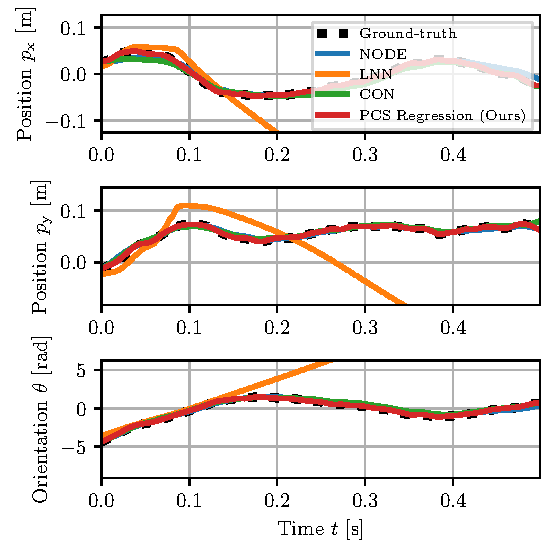
\includegraphics[width=0.49\textwidth]{pcsregression/figures/pcs_ns-2_with_baselines/rollout_train_marker_8.pdf}}
    \subfigure[Train: Marker $s=\SI{119}{mm}$]{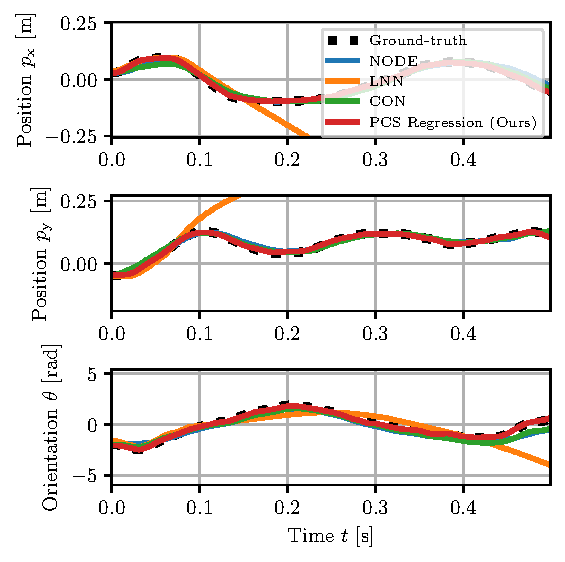
\includegraphics[width=0.49\textwidth]{pcsregression/figures/pcs_ns-2_with_baselines/rollout_train_marker_14.pdf}}\\
    \subfigure[Train: Marker $s=\SI{170}{mm}$ (EE)]{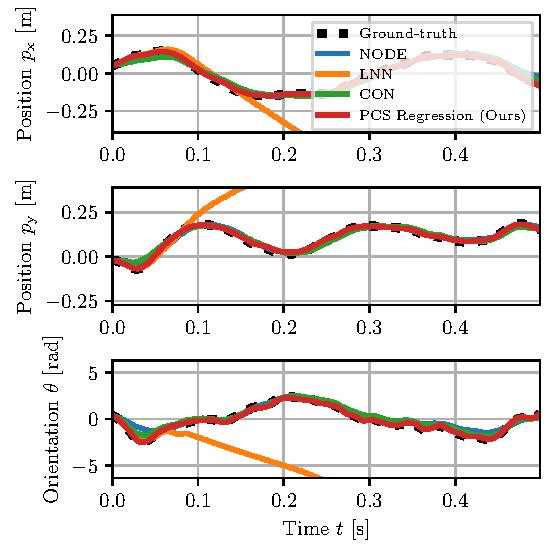
\includegraphics[width=0.49\textwidth]{pcsregression/figures/pcs_ns-2_with_baselines/rollout_train_marker_20.pdf}}
    \subfigure[Train: Actuation torques]{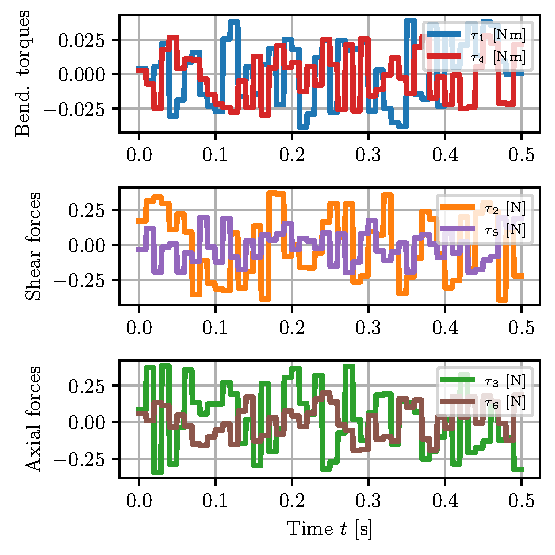
\includegraphics[width=0.49\textwidth]{pcsregression/figures/pcs_ns-2_with_baselines/torque_train.pdf}}

    \caption{Benchmarking of the proposed method against various machine learning baselines on a PCS soft robot consisting of two segments (\emph{Case 2}) on the \textbf{train dataset}: We train the baseline methods on the dynamical evolution of the Cartesian SE(2) poses of three \emph{markers} distributed over the backbone of the soft robot with a total length of \SI{170}{mm}. The upper and lower rows visualize the rollout of all methods on the training and the test set, respectively. The first three columns show the evolution of each of the three markers, where the last marker represents the end-effector. The last column displays the actuation torques that were used to generate the datasets.}
    \label{fig:pcsregression:dynamics_pcs_ns-2_with_baselines:training}
\end{figure}
\begin{figure}[ht]
    \centering
    \subfigure[Test: Marker $s=\SI{68}{mm}$]{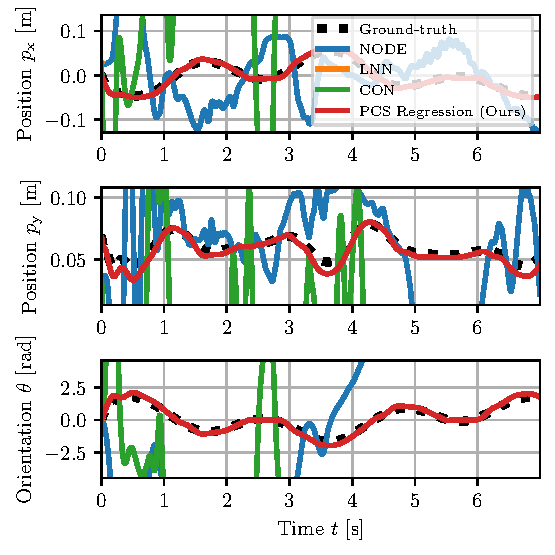
\includegraphics[width=0.49\textwidth]{pcsregression/figures/pcs_ns-2_with_baselines/rollout_val_marker_8.pdf}}
    \subfigure[Test: Marker $s=\SI{119}{mm}$]{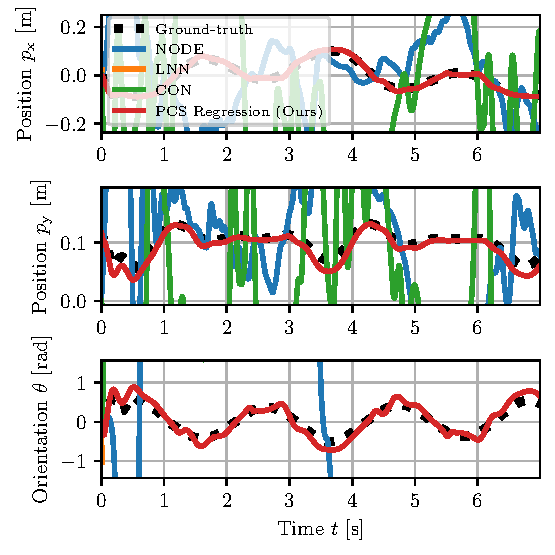
\includegraphics[width=0.49\textwidth]{pcsregression/figures/pcs_ns-2_with_baselines/rollout_val_marker_14.pdf}}\\
    \subfigure[Test: Marker $s=\SI{170}{mm}$ (EE)]{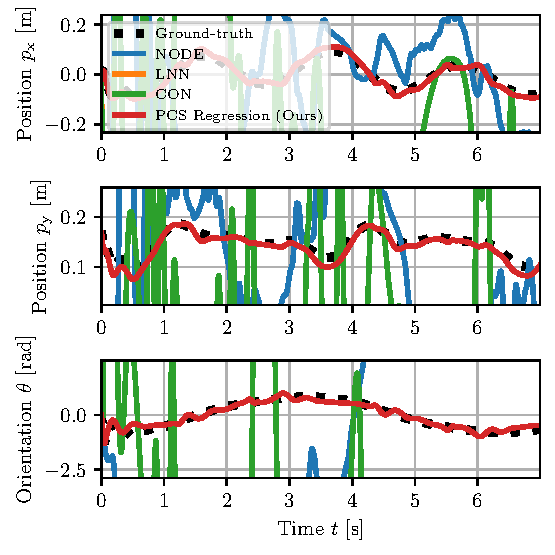
\includegraphics[width=0.49\textwidth]{pcsregression/figures/pcs_ns-2_with_baselines/rollout_val_marker_20.pdf}}
    \subfigure[Test: Actuation torques]{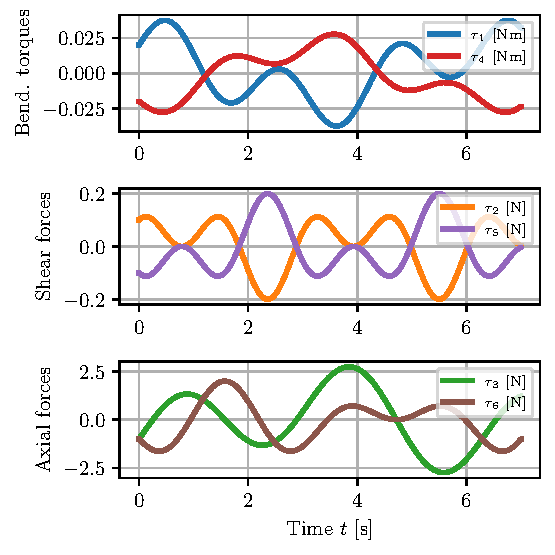
\includegraphics[width=0.49\textwidth]{pcsregression/figures/pcs_ns-2_with_baselines/torque_val.pdf}}

    \caption{Benchmarking of the proposed method against various machine learning baselines on a PCS soft robot consisting of two segments (\emph{Case 2}) on the \textbf{test dataset}: We train the baseline methods on the dynamical evolution of the Cartesian SE(2) poses of three \emph{markers} distributed over the backbone of the soft robot with a total length of \SI{170}{mm}. The upper and lower rows visualize the rollout of all methods on the training and the test set, respectively. The first three columns show the evolution of each of the three markers, where the last marker represents the end-effector. The last column displays the actuation torques that were used to generate the datasets.}
    \label{fig:pcsregression:dynamics_pcs_ns-2_with_baselines:test}
\end{figure}
% \begin{figure}[hbt]
%     \centering

%     \subfigure[Train: End-effector poses]{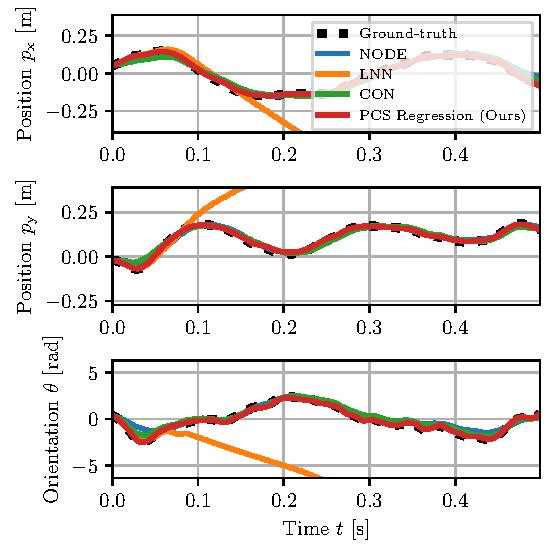
\includegraphics[width=0.49\columnwidth]{pcsregression/figures/pcs_ns-2_with_baselines/rollout_train_marker_20.pdf}}
%     \subfigure[Train: Actuation torques]{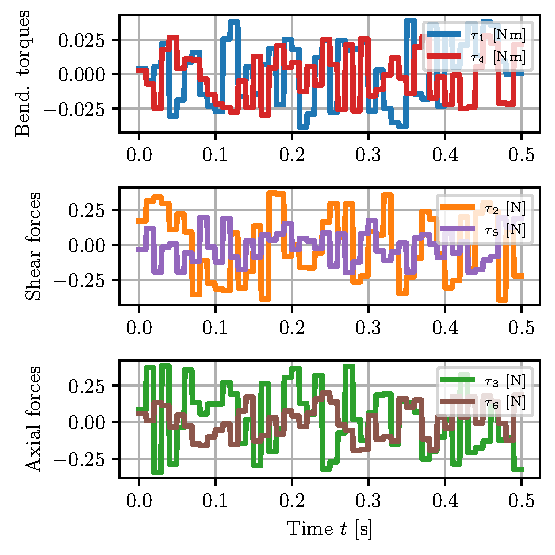
\includegraphics[width=0.49\columnwidth]{pcsregression/figures/pcs_ns-2_with_baselines/torque_train.pdf}}\\
%     \subfigure[Test: End-effector poses]{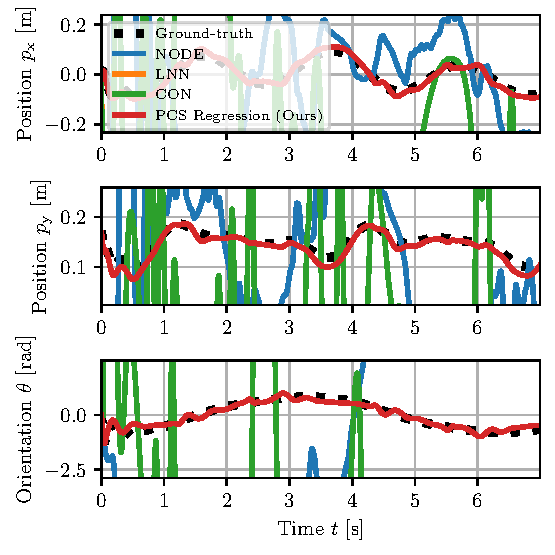
\includegraphics[width=0.49\columnwidth]{pcsregression/figures/pcs_ns-2_with_baselines/rollout_val_marker_20.pdf}}
%     \subfigure[Test: Actuation torques]{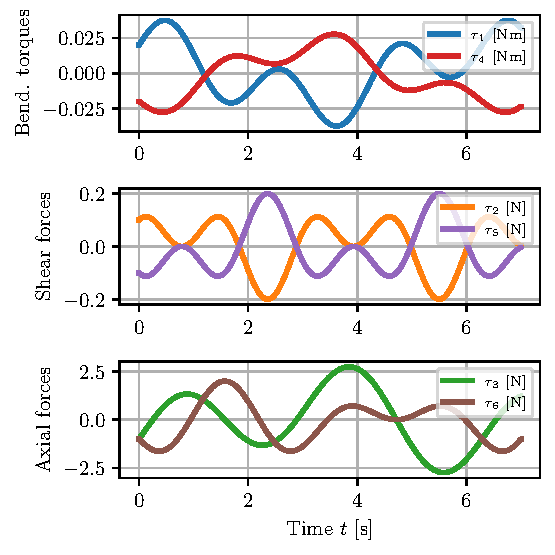
\includegraphics[width=0.49\columnwidth]{pcsregression/figures/pcs_ns-2_with_baselines/torque_val.pdf}}

%     \caption{Benchmarking of the proposed method against various machine learning baselines on a PCS soft robot consisting of two segments (\emph{Case 2}): We train the baseline methods on the dynamical evolution of the Cartesian SE(2) poses of three \emph{markers} distributed over the backbone of the soft robot with a total length of \SI{170}{mm}. The upper and lower rows visualize the rollout of all methods on the training and the test set, respectively. The first column shows the evolution end-effector pose. The last column displays the actuation torques that were used to generate the datasets.}
%     \label{fig:pcsregression:dynamics_pcs_ns-2_with_baselines}
% \end{figure}

\begin{table}[htbp]
\centering
%\renewcommand{\arraystretch}{1.3} % Increase space between rows
\caption{Results for learning dynamics of a two-segment PCS soft robot (Case 2). We report the position ($e_\mathrm{p}^\mathrm{body}$) and orientation ($e_\theta^\mathrm{body}$) metrics that capture the mean shape error averaged over all time steps. The shape error is computed by considering the dynamical evolution of three marker poses with $s_j \in \{ 68, 119, 170 \}$~\si{mm}. We report the metrics for a rollout of the dynamics on both a \SI{0.5}{s} sequence on the training set and the entire (i.e., \SI{7}{s}) test set.}
\label{tab:pcsregression:dynamics_pcs_ns-2_with_baselines}
\setlength\tabcolsep{3pt}
\begin{small}
\begin{tabular}{c r r r r}
    \toprule
    \textbf{Method} & \textbf{Train} $\mathbf{e_\mathrm{p}^\mathrm{body}}$ & \textbf{Train} $\mathbf{e_\theta^\mathrm{body}}$ & \textbf{Test} $\mathbf{e_\mathrm{p}^\mathrm{body}}$ & \textbf{Test} $\mathbf{e_\theta^\mathrm{body}}$\\
    \midrule
    \gls{NODE} & \SI{10.4}{mm} & \SI{0.27}{rad} & \SI{245.6}{mm} & \SI{12.22}{rad}\\
    \gls{LNN}~\citep{liu2024physics} & \SI{550.8}{mm} & \SI{5.16}{rad} & $\infty$ & $\infty$\\
    \gls{CON}~\citep{stolzle2024input} & \SI{12.9}{mm} & \SI{0.24}{rad} & \SI{789.5}{mm} & \SI{29.49}{rad}\\
    \textbf{PCS Regression (Ours)} & $\mathbf{3.1}$~\si{mm} & $\mathbf{0.04}~\si{rad}$ & $\mathbf{9.8}$~\si{mm} & $\mathbf{0.13}~\si{rad}$\\
    \bottomrule
\end{tabular}
\end{small}
\end{table}

\subsection{Benchmarking of Identified Dynamics against ML Baselines}
We benchmark the derived dynamical model of \emph{Case 2} (i.e., a two-segment planar \gls{PCS} soft robot) against several models trained using machine learning approaches. Specifically, we consider various learning-based approaches that range from completely data-driven (e.g., \gls{NODE}) over approaches that take into account the structure of Lagrangian systems (e.g., \gls{LNN}, \gls{CON}).
% To keep the comparison fair, we define the task as learning the dynamical evolution of the backbone without any access to prior information about the kinematics (e.g., no knowledge about number of segments, length of each segment, active strains, etc.).
To keep the comparison fair, we define the inputs for all methods as the Cartesian poses $\chi_j \in \mathbb{R}^3$ and the corresponding time derivative $\dot{\chi}_j$ of $N$ discrete \emph{markers} along the backbone. Furthermore, we also provide the actuation torques $\tau \in \mathbb{R}^6$ as a dynamic model input. Therefore, the total model input exhibits a dimensionality of $\mathbb{R}^{6N + 6}$. The task of the dynamic model is to predict the acceleration $\ddot{\chi}(k) \in \mathbb{R}^{3N}$. % (\gls{NODE}, \gls{CON}, \gls{LNN}). % or next state $(\chi(k+1), \dot{\chi}(k+1)) \in \mathbb{R}^{18}$ (\gls{LSTM}) of all markers.
We tried supplying all $21$ markers, which our method also has access to, to the baseline approaches. However, this proved to be infeasible as the problem would become too high-dimensional in terms of the number of inputs and outputs, and the baseline approaches would overfit the training set. Therefore, we settled to give the baseline methods access to the pose measurements of $N=3$ markers distributed along the backbone of the robot at $s_j \in \{ 68, 119, 170 \}$~\si{mm}, where $s=\SI{170}{mm}$ corresponds to the end-effector.

\paragraph{Implementation of Baseline Methods}
The \gls{NODE} is parametrized by a six-layer \gls{MLP} with hidden dimension $256$ and hyperbolic tangent activation function that predicts based on the input $(\chi(t), \dot{\chi}(t), \tau(t))$ the acceleration $\ddot{\chi}$. We remark that with this strategy, we already infuse the prior knowledge that the time derivative of the pose is the velocity, which would not be the case in a naive implementation of a \gls{NODE}.
\glspl{CON}~\citep{stolzle2024input} allow for learning of (latent) dynamics of Lagrangian systems with strong stability guarantees (global asymptotic stability / input-to-state stability) by leveraging a network of damped harmonic oscillators that are coupled by a hyperbolic potential. In order to allow for arbitrary placement of the global asymptotically stable equilibrium point, we learn a linear coordinate transformation into the latent coordinates $z = W \chi + b \in \mathbb{R}^9$, $\dot{z} = W \dot{\chi}$. % After the latent acceleration $\ddot{z}$ is predicted by the \gls{CON} network, we can project it back into Cartesian space as $\ddot{\chi} = W^{-1} \ddot{z}$. 
% We parametrize the actuation to oscillator forcing mapping $V(\tau) \in \mathbb{R}^{6 \times 9}$ with a five-layer MLP with hidden dimension $16$ (\texttt{tanh} activation).
\glspl{LNN} learn the components of the Lagrangian $\mathcal{L}(\chi, \dot{\chi}) = \frac{1}{2} \dot{\chi}^\top M(\chi) \dot{\chi} - \mathcal{U}(\chi)$ such as the mass matrix $M(\chi) \succ 0 \in \mathbb{R}^{9 \times 9}$, the potential energy $\mathcal{U}(\chi) \in \mathbb{R}$, the damping matrix $D \succeq 0 \in \mathbb{R}^{9 \times 9}$ and the actuation matrix $A \in \mathbb{R}^{6 \times 9}$ and subsequently derive the \gls{EOM} as $M(\chi) \ddot{\chi} + \frac{\partial \mathcal{L}}{\partial \chi \partial \dot{\chi}} \dot{\chi} + \frac{\partial \mathcal{U}}{\partial \chi} + D \dot{\chi} = A \tau$ using autodifferentiation.
We regard $A$ and $D$ as trainable weights and parametrize $M(\chi)$ and $\mathcal{U}(\chi)$ with six-layer \glspl{MLP} with hidden dimension $256$ (softplus activation). We leverage the Cholesky decomposition to make sure that $M(\chi), D \succ 0$.

\paragraph{Training}
% We split off the last \SI{20}{\percent} of the training set trajectory as the validation set.
% Analog to how the dynamic regression of our proposed method is implemented, the natural way would be to train the baseline methods (e.g., \gls{NODE}, \gls{CON}, \gls{LNN}) to directly predict the acceleration $\hat{\ddot{\chi}}(t)$ for every dataset input tuple $(\chi(k), \dot{\chi}(k), \tau(k))$.
% Then, we would apply a supervised training loss (e.g., \gls{MSE}) between the predicted acceleration and the corresponding label $\ddot{\chi}(k)$, which is generated by numerically differentiating the pose trajectory.
% However, we found that even if the baseline models would accurately predict the accelerations on the validation loss, we would perform badly or even become unstable when rolled out over a mid-to-long time horizon (i.e., longer than approx. \SI{0.1}{s}).
% Therefore, even though this is not done for our proposed method, we additionally roll out the trajectories during training over a horizon of \SI{0.3}{s} and add loss terms that compute the \gls{MSE} error between the predicted states $(\hat{\chi}(k+r), \hat{\dot{\chi}}(k+r))$ and the training set states $(\chi(k+r), \dot{\chi}(k+r))$, where $r$ is the index of the rollout step.
The first loss term is a \gls{MSE} between the predicted $\hat{\ddot{\chi}}(k)$ and actual acceleration $\ddot{\chi}(k)$. Additionally, we roll out the trajectories over a horizon of \SI{0.3}{s} and add loss terms that compute the \gls{MSE} error between the predicted states $(\hat{\chi}(k+r), \hat{\dot{\chi}}(k+r))$ and the labels $(\chi(k+r), \dot{\chi}(k+r))$, where $r$ is the index of the rollout step.
As training \glspl{LNN} is computationally very demanding due to the need to differentiate w.r.t. both inputs and neural network parameters, we had to reduce the training rollout horizon. % restrict the horizon to \textcolor{orange}{\SI{0.01}{s}}.

\paragraph{Results}
We present the benchmarking results in Fig.~\ref{fig:pcsregression:dynamics_pcs_ns-2_with_baselines:training} (evaluation on the training set) and Fig.~\ref{fig:pcsregression:dynamics_pcs_ns-2_with_baselines:test} (evaluation on the test set). Quantitative error metrics are provided in Table~\ref{tab:pcsregression:dynamics_pcs_ns-2_with_baselines}.
We report the performance for rollouts on both the training and the test set.
All methods, except for \gls{LNN}, are able to predict the Cartesian-space evolution of the markers attached to the soft robot backbone decently accurately over the training set trajectory. Still, the our proposed method exhibits an \SI{70}{\percent} to \SI{80}{\percent} lower error than \gls{NODE} and \gls{CON}~\citep{stolzle2024input}. As \gls{LNN} does not exhibit any stability guarantees and it is trained on a relatively short horizon, it diverges from the ground-truth trajectory after roughly \SI{0.15}{s}.
As shown in panels (d) of Figs.~\ref{fig:pcsregression:dynamics_pcs_ns-2_with_baselines:training} and \ref{fig:pcsregression:dynamics_pcs_ns-2_with_baselines:test}, the axial actuation forces on the validation set are one order of magnitude higher than in the training set. Therefore, these axial forces can be considered to be out-of-distribution for the trained models. Our proposed method is amazingly able to still exhibit very good performance, while all baseline methods are no longer able to predict the dynamic evolution of the system. \gls{LNN} even becomes fully unstable after a few milliseconds, and we are, therefore, not able to report test errors for this method.

\begin{figure}[ht]
    \centering
    \subfigure[Bending strains]{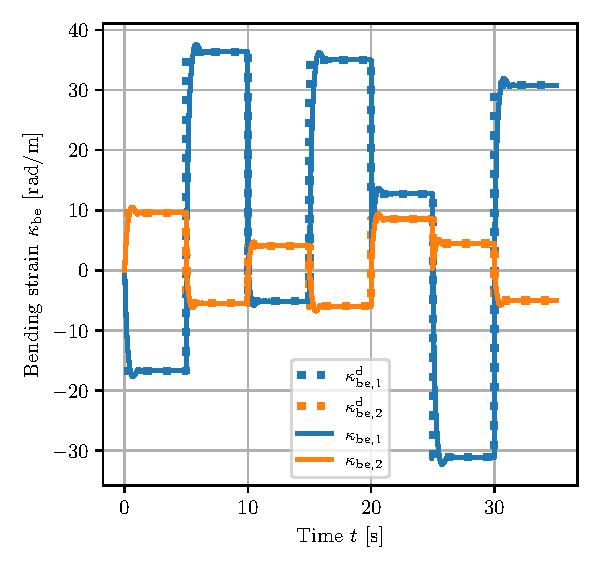
\includegraphics[width=0.4\columnwidth, trim={5 5 5 5}]{pcsregression/figures/control/setpoint_control_bending.pdf}}
    \subfigure[Linear strains]{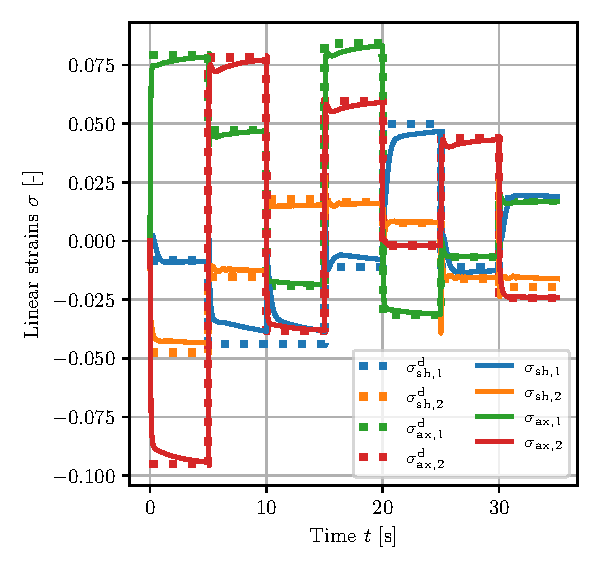
\includegraphics[width=0.4\columnwidth, trim={5 5 5 5}]{pcsregression/figures/control/setpoint_control_linear.pdf}}
    \caption{Demo of model-based control of a two-segment soft robot based on the learned dynamical model. We ask the controller to track a sequence of $7$ setpoints $q^\mathrm{d}\in \mathbb{R}^6$ which is denoted with dotted lines. The controller contains a feedforward and feedback term where the feedforward term compensates for the elastic and gravitational forces at the setpoint. 
    % We refer with $\kappa_{\mathrm{be},1}, \kappa_{\mathrm{be},2}$ to the bending strains of the first and second segment, respectively. Similarly, $\sigma_{\mathrm{sh},i}$ and $\sigma_{\mathrm{ax},i}$ represent the shear and axial strains.
    }
    \label{fig:pcsregression:results:control:pcs_ns-2}
\end{figure}

\subsection{Demonstration of Model-based Control}\label{sub:pcsregression:validation:model_based_control}
To demonstrate how the derived models can be used in a plug-and-play fashion for model-based control, we simulate the closed-loop dynamics of a simulated two-segment \gls{PCS} soft robot (\emph{Case 2}) with configuration $q \in \mathbb{R}^7$ under a P-satI-D+FF~\citep{della2023model, stolzle2024experimental, stolzle2024input} setpoint control policy
\begin{equation}
\begin{split}
    \tau(t, q) =& \: \underbrace{\hat{G}(q^\mathrm{d})+\hat{K}q^\mathrm{d}}_{\text{Learned feedforward term}} + \underbrace{K_\mathrm{p} \, (q^\mathrm{d} - q) - K_\mathrm{d} \, \dot{q} + K_\mathrm{i} \, e_\mathrm{int}(t) }_{\text{P-satI-D feedback term~\citep{pustina2022p}}},
\end{split}
\end{equation}
where $K_\mathrm{p}, K_\mathrm{i}, K_\mathrm{d} \in \mathbb{R}^{n \times n}$ are the proportional, integral, and derivative control gains, respectively.
The feedback control term is a PID-like controller with integral saturation~\citep{pustina2022p} and the dimensionless gain $\Upsilon \in \mathbb{R}$ which bounds the integral error at each time step to the interval $(-1, 1)$ and reduces the risk of instability for nonlinear systems
\begin{equation}
    e_\mathrm{int}(t, q) = \:  \int_0^t \tanh(\Upsilon (q^\mathrm{d}(t') - q(t'))) \: \mathrm{d}t',
\end{equation}
$\hat{G}(q) \in \mathbb{R}^{6}$ and $\hat{K} \in \mathbb{R}^{6 \times 6}$ are the estimated gravitational forces and stiffness matrix, respectively.
We simulate the closed-loop dynamics with a Tsitouras 5(4) integrator at a timestep of $\SI{0.05}{ms}$.
Please note that we use the ground-truth dynamics as a state transition function.
% After manual tuning, we select the control gains $K_\mathrm{p} = \mathrm{diag}(0.01, 0.5, 6, 0.01, 0.5, 6)$, $K_\mathrm{i} = \mathrm{diag}(0.06, 3, 36, 0.06, 3, 36)$, $K_\mathrm{d} = \mathrm{diag}(0.002, 0.1, 0.8, 0.002, 0.1, 0.8)$, and $\Upsilon = \mathrm{diag}(40, 0.1, 0.2, 40, 0.1, 0.2)$.

To verify that the learned model performs well within the model-based control policy, we create a sequence of $7$ randomly sampled setpoints $q^\mathrm{d}(k) \in \mathbb{R}^6$. % $} \in \mathcal{U}([-\SI{40}{rad \per m}, ], [])$.
The results in Fig.~\ref{fig:pcsregression:results:control:pcs_ns-2} show that the controller is able to effectively regulate a two-segment planar soft robot. %  that exhibits bending, shear, and axial strains.
The tracking of the bending strain reference is perfect. For the linear strains, we notice small errors in the feedforward term, but the integral control is able to compensate for them and drive the system toward the reference.
We stress that the structure and characteristics of the learned model enabled us to formulate the control policy in closed form easily, and we did not have to resort to techniques such as \gls{MPC} or \gls{RL} as it would be necessary for other model learning techniques (e.g., \glspl{LSTM}, \glspl{NODE}).
% \section{Conclusion}
% In this work, we present a data-driven method that utilizes the PCS strain model to derive low-dimensional kinematic and dynamic models for continuum soft robots from discrete backbone pose measurements, outperforming ML-based models like neural networks by maintaining the physical robot structure. This enhancement improves data efficiency and performance beyond the training set, allowing for direct and effective model-based control design. 
% %Unlike traditional methods that require extensive expert input and complex identification processes, our approach automates the determination of key model parameters using a robust linear least-squares regression, providing significant efficiency gains. 
% %We validated our learned models through simulations that demonstrated their ability to accurately predict robot dynamics and control from minimal data inputs, showing superior accuracy and generalization capabilities compared to existing methods. 
% Future work will explore expanding this approach to 3D models and real-world applications, aiming to further refine the actuation matrix for underactuated systems.

\section{Conclusion}
In this work, we propose a data-driven approach leveraging the \gls{PCS} strain model to identify low-dimensional kinematic and dynamic models for continuum soft robots directly from discrete pose measurements of the backbone's shape.
Compared to \gls{ML}-based models (e.g., neural networks, symbolic regression), we preserve the physical structure of the continuum soft robot model, leading to a significantly improved training data efficiency and out-of-training-distribution performance.
Furthermore, our method preserves the physical structure, enabling fast and efficient model-based control design.
Compared to deriving and formulation continuum soft robot models by hand using \gls{PCC}, \gls{PCS}, etc. approximations, our approach requires (i) less expert knowledge as the number of segments, segment lengths, active strains, etc. are automatically determined and (ii) we are able to regress all dynamic parameters with closed-form linear least-squares which is more efficient and robust than traditionally used system identification procedures (e.g., constrained nonlinear least squares, determination of parameters using mechanical testing equipment).

We verified both the \emph{Kinematic Fusion} and the \emph{Dynamic Regression and Sparsification} algorithms in simulation. The \emph{Kinematic Fusion} method can automatically and accurately determine the number of planar \gls{PCS} segments and their respective length purely based on extracted SE(2) poses of the backbone shape. 
For continuum soft robots whose shape by definition cannot be represented by the \gls{PCS} model (e.g., soft robots exhibiting affine curvature), we formulated a Pareto front between the \gls{DOF} of the model and the shape reconstruction accuracy. This enables the user to easily choose the best kinematic model for a given computational budget.
We showed that our proposed method is able to derive very accurate dynamic models from just \SI{4}{s} of video recordings and can generalize to out-of-distribution actuation sequences, which is not the case for the \gls{ML}-based baseline methods that we considered (e.g., \gls{NODE}, \gls{LNN}~\cite{liu2024physics}, and \gls{CON}~\cite{stolzle2024input}).
Furthermore, even for samples inside the training distribution, our method exhibits a more than \SI{70}{\percent} lower shape prediction error than the baselines.
Finally, we demonstrated that the physical structure of the dynamical model that remains intact during the regression allows us to leverage the learned dynamics within closed-form model-based control in a plug-and-play fashion.
For future work, it would be interesting to validate the proposed approach on both 3D (i.e., $SE(3)$ input poses) and real-world data. Furthermore, it would be valuable to identify ways to regress a possibly underactuated actuation matrix $A(q) \in \mathbb{R}^{n_\mathrm{q} \times m}$, where $m$ is the number of actuators.


\section*{Afterword}
In this chapter, we presented a data-driven approach for identifying strain-based models for continuum soft robots. Crucially, we preserve all insight and physical interpretability into the kinematic and dynamical models, respectively. These features enable us to \emph{debug} the model and apply the fundamentally the same model-based control concepts (e.g., P-satI-D+feedforward) that we previously used in Chapter~\circled{\ref{chp:hsacontrol}} for the \gls{HSA} robot. Furthermore, the strain distance threshold in the \emph{Kinematic Fusion} algorithm and the maximum stiffness threshold in the \emph{Strain Sparsification} algorithm allow us to make the tradeoff between model complexity and model performance (i.e., shape reconstruction for the kinematic model and prediction accuracy for the dynamic model) explicit.
As we basically derive an entirely \emph{whitebox} model, the dynamic model exhibits excellent extrapolation performance compared to \emph{blackbox} or even \emph{greybox} (e.g., \glspl{LNN}) \gls{SOTA} \gls{ML} techniques.
% However, even though the approach presented in this chapter exhibits excellent performance and generates low-dimensional control-oriented models, it is not sufficient to learn and incorporate very complex soft robot behavior, such as deformations of the backbone cross-sections, which the Cosserat rod model neglects or time-dependent effects such as hysteresis. Additional model features such as nonlinear elasticity, as present for \gls{HSA} robots, could theoretically be backed into the model but could not be automatically detected by the algorithm presented in this chapter.
% Furthermore, as the approach uses a \gls{PCS}-based parametrization which is in turn derived from the Cosserat rod theory, it would exhibit inferior performance for robots where the \emph{slender rod} assumption is not met anymore.
% Finally, the problem setting presented in this chapter considers that pose samples of the shape of the backbone are available.
% However, exteroceptive sensing modalities such as motion capture systems are not practical in a future where we seek soft robots to assist humans with activities of daily living and to extract the backbone shape with computer vision is prone to errors, particularly in situations where tracking of key points along the soft robot body across time is challenging.
% Consequently, we present in Chapter~\ref{chp:con} an approach that leverages a network of the most basic mechanical system (i.e., a harmonic oscillator) for learning latent dynamics from image pixels.
% This approach can be seen as a \emph{greybox} model where both the reduced-order coordinates (approximated by an autoencoder) and the dynamical system (approximated with a \gls{CON}) are learned using modern \gls{ML} techniques but we preserve a mechanical interpretation of both latent variables and latent dynamics. This allows us to analyze the characteristics of the learned latent system (e.g., the kinetic and potential energy) and subsequently also exploit this knowledge for model-based control in latent space.
Although the approach presented in this chapter demonstrates excellent performance and produces low-dimensional, control-oriented models, it cannot capture very complex soft robot behaviors. These include deformations of the backbone cross-sections, which the Cosserat rod model neglects, as well as time-dependent effects such as hysteresis. While features like nonlinear elasticity, observed in \gls{HSA} robots (see Chapter~\ref{chp:hsamodel}), could theoretically be integrated into the model, they currently cannot be automatically identified by the algorithm introduced in this chapter.
Additionally, since the approach relies on a \gls{PCS}-based parametrization derived from Cosserat rod theory, it performs poorly for robots that do not satisfy the \emph{slender rod} assumption. Moreover, the problem setting assumes access to pose samples of the backbone’s shape. However, in scenarios where soft robots are intended to assist humans with daily activities, exteroceptive sensing methods like motion capture systems become impractical. Extracting the backbone shape using computer vision is also prone to errors, especially when tracking key points along the soft robot’s body over time is challenging. 

Therefore, in Chapter~\circled{\ref{chp:con}}, we propose an alternative approach that employs a network of basic mechanical systems (e.g., a harmonic oscillator) to learn latent dynamics directly from image pixels. This method can be viewed as a \emph{grey-box} model, where both the reduced-order coordinates (approximated by an autoencoder) and the dynamical system (approximated by a \gls{CON}) are learned using modern \gls{ML} techniques. Crucially, this approach retains a mechanical interpretation of both latent variables and their dynamics, enabling analysis of the learned latent system’s properties (e.g., kinetic and potential energy). This insight can then be leveraged for model-based control within the latent space.